
\documentclass[12pt,PhD,twoside,openright]{muthesis}

% Packages MU
\usepackage{verbatim}
\usepackage{graphicx}
\usepackage{url} % typeset URL's reasonably
\def\UrlBreaks{\do\/\do-}
\usepackage{listings}

\usepackage{pslatex} % Use Postscript fonts
\usepackage[toc]{}
% Uncomment this to use a glossary
% \usepackage[toc]{glossaries}
% \input{./glossary}
% \makeglossaries

%%%%%%%%%%%%%%%%%%%%%%
\usepackage{graphicx,latexsym}
\usepackage{amsmath}
\usepackage{amssymb,amsthm}
\usepackage{longtable,booktabs,setspace}
% \usepackage{chemarr} %% Useful for one reaction arrow, useless if you're not a chem major
% \usepackage[hyphens]{url}
% Added by CII
\usepackage[anythingbreaks]{}
\usepackage{hyperref}
\hypersetup{colorlinks = false}
\renewcommand{\UrlBreaks}{\do\/\do\a\do\b\do\c\do\d\do\e\do\f\do\g\do\h\do\i\do\j\do\k\do\l\do\m\do\n\do\o\do\p\do\q\do\r\do\s\do\t\do\u\do\v\do\w\do\x\do\y\do\z\do\A\do\B\do\C\do\D\do\E\do\F\do\G\do\H\do\I\do\J\do\K\do\L\do\M\do\N\do\O\do\P\do\Q\do\R\do\S\do\T\do\U\do\V\do\W\do\X\do\Y\do\Z\do\0\do\1\do\2\do\3\do\4\do\5\do\6\do\7\do\8\do\9\do\%\do\.\do\-}

\renewcommand{\chapterautorefname}{Chapter}

\usepackage{lmodern}
\usepackage{float}
\floatplacement{figure}{H}
% End of CII addition
\usepackage{rotating}



\usepackage{natbib}
%%% --- The following two lines are what needs to be added --- %%%
%\setcounter{biburllcpenalty}{7000}
%\setcounter{biburlucpenalty}{8000}
% Comment out the natbib line above and uncomment the following two lines to use the new
% biblatex-chicago style, for Chicago A. Also make some changes at the end where the
% bibliography is included.
%\usepackage{biblatex-chicago}
%\bibliography{thesis}


% Added by CII (Thanks, Hadley!)
% Use ref for internal links
% \renewcommand{\hyperref}[2][???]{\autoref{#1}}
% \def\chapterautorefname{Chapter}
% \def\sectionautorefname{Section}
% \def\subsectionautorefname{Subsection}
% End of CII addition

% Added by CII
\usepackage{caption}
% \captionsetup{width=5in}
% End of CII addition

% \usepackage{times} % other fonts are available like times, bookman, charter, palatino

% Syntax highlighting #22




% if you're writing a thesis in an interdisciplinary major,
% uncomment the line below and change the text as appropriate.
% check the Senior Handbook if unsure.
%\thedivisionof{The Established Interdisciplinary Committee for}
% if you want the approval page to say "Approved for the Committee",
% uncomment the next line
%\approvedforthe{Committee}

% Added by CII
%%% Copied from knitr
%% maxwidth is the original width if it's less than linewidth
%% otherwise use linewidth (to make sure the graphics do not exceed the margin)
% \makeatletter
% \def\maxwidth{ %
%   \ifdim\Gin@nat@width>\linewidth
%     \linewidth
%   \else
%     \Gin@nat@width
%   \fi
% }
% \makeatother

% \renewcommand{\contentsname}{Table of Contents}
% End of CII addition

% \setlength{\parskip}{0pt}

% Added by CII
% 
\providecommand{\tightlist}{%
  \setlength{\itemsep}{0pt}\setlength{\parskip}{0pt}}

	\newcommand{\txt}[1]{\textrm{#1}}

 \def\logit{\txt{logit}}

 \newcommand{\sfrac}[2]{\;^{#1}/_{#2}}
	
 \usepackage{amsmath}
 \usepackage[T1]{fontenc}
 \usepackage{rotating}
 \usepackage{booktabs}
 \usepackage{longtable}
 \usepackage{array}
 \usepackage{multirow}
 \usepackage{wrapfig}
 \usepackage{float}
 \usepackage{colortbl}
 \usepackage{pdflscape}
 \usepackage{tabu}
 \usepackage{threeparttable}
 \usepackage{threeparttablex}
 \usepackage[normalem]{ulem}
 \usepackage{makecell}
 \usepackage{xcolor}
 \usepackage{geometry}
 \usepackage{fancyhdr}

\newlength{\cslhangindent}
\setlength{\cslhangindent}{1.5em}
\newenvironment{cslreferences}%
  {}%
  {\par}
  

\begin{document}

\title{Multi-State Clinical Prediction Models in Renal Replacement Therapy}
\author{Michael Andrew Barrowman}
\principaladviser{}
\faculty{}
\school{}
\beforeabstract

\prefacesection{Abstract}
Insert Abstract Here\ldots{}

\afterabstract

\prefacesection{Acknowledgements}

\begingroup

\setlength{\parskip}{15pt}
\setlength{\parindent}{0pt}
Insert Ackowledgements Here\ldots{}

\par
\endgroup
\afterpreface

\hypertarget{introduction}{%
\chapter*{Introduction}\label{introduction}}
\addcontentsline{toc}{chapter}{Introduction}

Welcome to my Thesis. I've used R Markdown to create a gitbook style thesis, as well as a traditional pdf (following the UoM Thesis template). The html version can be found \href{https://michaelbarrowman.co.uk/thesis}{here}.

I sent an email with details of how you can log in to the \href{https://hypothes.is/}{hypothes.is} system. This will let you add comments to the gitbook pages. This is actually a really useful tool and has the ability to add annotations to any webpage. Annotated text can be seen highlighted and to add your own, just highlight the text you want to comment on, and the annotate bubble pops up (try it now). Make sure you click Post to Public after writing the annotation and annotations can include Rich Text and Markdown. You can view Annotations by clicking the menu on the right and this will show all comments.

Google Docs was great, but when I started to use R Markdown for other purposes, I realised I could embed tables and equations much easier and automatically using \texttt{kable}. Google Docs on it's own became rather clunky (especially with tables, just like Word) and whenever I updated a document using R Markdown, any comments that were added to the document were lost. It was also difficult for you to remember \emph{where} each document lived. Since R Markdown can also output to \texttt{LaTeX} I thought it would be easier to collate papers together. I'd have had to do this kind of transition over to\texttt{LaTeX} for my thesis eventually and this would have been difficult and tedious from Google Docs or Word.

Importantly, I've also added in functionality to output each chapter individually. For unpublished papers, there will be a link to download the pdf and tex versions of the individual paper.

Everything here is hosted in a \href{https://https://github.com/MyKo101/Thesis}{Github repo}. I originally used Github as my backup, but then decided to increase how I used it.

\hypertarget{chap-lit-report}{%
\chapter{Literature Report}\label{chap-lit-report}}

\chaptermark{Literaure Report}

Last updated: 01 May

\hypertarget{introduction-1}{%
\section{Introduction}\label{introduction-1}}

\hypertarget{clinical-prediction-models}{%
\section{Clinical Prediction Models}\label{clinical-prediction-models}}

The idea of prognosis dates back to ancient Greece with the work of Hippocrates {[}\protect\hyperlink{ref-hippocrates_genuine_1886}{1}{]} and is derived from the Greek for ``know before'' meaning to forecast the future. Within the sphere of healthcare, it is definde as the risk of future health outcomes in patients, particularly patients with a certain disease or health condition. Prognosis allows clinicians to provide patients with a prediction of how their disease will progress and is uaully given as a probability of having an event in a prespecified number of years. For example, QRISK3 {[}\protect\hyperlink{ref-hippisley-cox_development_2017}{2}{]} provides a probability that a patient will have a heart attack or stroke in the next 10 years. Prognostic research encompasses any work which enhances the field of prognosis, whether through methodological advancements, field-specific prognostic modelling or educational material designed to improve general knowledge of prognosis. Prognostic models come under the wider umbrella of predictive models which also includes diagnostic models; because of this most of the keys points in the field or prognostic modeling can be applied to diagnostic models with little to no change.

Prognosis allows clinicians to evaluate the natural history of a patient (i.e.~the course of a patient's future without any intervention) in order to establish the ffect of screening for asymptomatic diseases (such as with mammograms{[}\protect\hyperlink{ref-hemingway_prognosis_2013}{3}{]}). Prognosis research can be used to develop new definitions of diseases, whether a redefinition of an existing disease (such as the extension to th definition of myocardial infarction to include non-fatal events {[}\protect\hyperlink{ref-thygesen_universal_2007}{4}{]}) or a previously unknown subtype of a disease (such as Brugada syndrome as a type of cardiovascular disease{[}\protect\hyperlink{ref-probst_long-term_2010}{5}{]})

In general, prognosis research can be broken down into four main categories, with three subcategories {[}\protect\hyperlink{ref-riley_prognosis_2019}{6}{]}:
\begin{itemize}
\tightlist
\item
  Type I: Fundamental prognosis research {[}\protect\hyperlink{ref-hemingway_prognosis_2013}{3}{]}
\item
  Type II: Prognostic factor research {[}\protect\hyperlink{ref-riley_prognosis_2013}{7}{]}
\item
  Type III: Prognostic model research {[}\protect\hyperlink{ref-steyerberg_prognosis_2013}{8}{]}
  \begin{itemize}
  \tightlist
  \item
    Model development {[}\protect\hyperlink{ref-royston_prognosis_2009}{9}{]}
  \item
    Model validation {[}\protect\hyperlink{ref-altman_prognosis_2009}{10}{]}
  \item
    Model impact evaluation {[}\protect\hyperlink{ref-moons_prognosis_2009}{11}{]}
  \end{itemize}
\item
  Type IV: Stratified Medicine {[}\protect\hyperlink{ref-hingorani_prognosis_2013}{12}{]}
\end{itemize}
For a particular outcome, prognostic research will usually progress through these types, beginning with papers designed to evaluate overall prognosis within a whole population and then focusing in on more specificity and granularity towards individualised, causal predictions.

The model development and validation will usually occur in the same paper {[}\protect\hyperlink{ref-collins_transparent_2015}{13}{]}, {[}\protect\hyperlink{ref-moons_transparent_2015}{14}{]}. studies into all three of the subcategories of prognostic model research \emph{should} be completed before a model is used in clinical practice {[}\protect\hyperlink{ref-riley_external_2016}{15}{]}, although this does not always occur {[}\protect\hyperlink{ref-steyerberg_prognosis_2013}{8}{]}. External validation is considered by some to be more important than the actual deviration of the model as it demonstrates generalisability of the model {[}\protect\hyperlink{ref-collins_systematic_2013}{16}{]}, whereas a model on it's own may be highly susceptible to overfitting {[}\textbf{Cite: Something}{]}.

\hypertarget{fundamental-prognosis-research}{%
\subsection{Fundamental Prognosis Research}\label{fundamental-prognosis-research}}

{[}\textbf{What is it? Old definition is incorrect, so will need to write this fresh}{]}

\hypertarget{prognostic-factor-research}{%
\subsection{Prognostic Factor Research}\label{prognostic-factor-research}}

The aim of prognostic factor research (Type II) is to discover which factors are associated with disease progression. This allows for the general attribution of relationships between predictors and clinical outcomes.

Predictive factor research can give researchers and clinicians an idea of which patient factors are important when assessing a disease. It is vital to the development of clinical predictive models as without an idea of what covariates \emph{can} affect an outcome, we cannot figure out which variables \emph{will} affect the outcome. For example, {[}\textbf{xxxx}{]} demonstrated that {[}\textbf{xxxx}{]} is correlated with {[}\textbf{xxxx}{]}, which subsequently used as a covariate in the development of the {[}\textbf{xxxx}{]} model. Note the use of the word correlate here as prognostic relationships do not have to be causal ones {[}\textbf{Cite: Something}{]}. These factors may indeed represent an underlying causal pathway, but this is not a requirement and it would require aetiological methods to discern whether it were causal or not. For example, when predicting {[}\textbf{xxxx}{]}, we can demonstrate that {[}\textbf{xxxx}{]} is a prognostic factor, {[}however since the arrow of causation is {[}\textbf{xxxx}{]}{]} {[}\textbf{OR}{]} {[}however since {[}\textbf{xxxx}{]} causes both {[}\textbf{xxxx}{]} and {[}\textbf{xxxx}{]}{]}, the relationship is prognostic, but not causal. {[}\textbf{Previously used Apgar score here, reference 40}{]}

Counter to the idea that prognostic factors aren't always causal, they are \emph{always} confounding factors for the event they predict. Thue prognostic factors should be taken into account when planning clinical trials as if they are wildly misbalanced across the arms (or not accounted for in some other manner), they can cause biases in the results {[}\protect\hyperlink{ref-riley_prognosis_2013}{7}{]}. Sometimes these factors are so strong that adjusting the results of a clinical trial by the factor can affect, or even reverse the interpretation of the results {[}\protect\hyperlink{ref-royston_dichotomizing_2006}{17}{]}. If a prognostic factor is causal, then by directly affecting the factor, it can causally affect the outcome. By discovering new prognostic factors, and investigating their causality, we can potentially open the door to new directions of attack for treatments.

It is unfortunate, however, that Riley at al {\textbf{???}} found that only 35.5\% of prognostic factor studies in paediatric oncology actually reported the size of the effect of the prognostic factor they reported on. This means that very little information can be drawn from these studies. It is also important that prognostic factor research papers consider and report on the implications of the factor they assess such as healthcare costs. These kinds of implications are rarely assessed, especially when compared to drugs or interventions {[}\protect\hyperlink{ref-riley_prognosis_2013}{7}{]}.

\hypertarget{prognostic-model-research}{%
\subsection{Prognostic Model Research}\label{prognostic-model-research}}

Predictive factors can be combined into a predictive model, which is a much more specific measurement of the effect of a factor on an outcome {[}\protect\hyperlink{ref-steyerberg_prognosis_2013}{8}{]} and they are deigned to augment the job of a clinician; and not to completely replace them {[}\protect\hyperlink{ref-moons_prognosis_2009}{11}{]}. Diagnostic prediction model can be used to indicate whether a patient is likely to need further testing to establish the presence of a disease {[}\protect\hyperlink{ref-collins_transparent_2015}{13};\textasciitilde moons\_transparent\_2015{]}. Prognostic prediction models can be used to decide on further treatment for that patient, whether as a member of a certain risk group, or under a stratied medicine approach {[}\protect\hyperlink{ref-collins_transparent_2015}{13}{]}, {[}\protect\hyperlink{ref-moons_transparent_2015}{14}{]}. Outcomes being assessed in a prediction model should be directly relevant to the patient (such as mortality) or have a direct causal relationship with something that is {[}\protect\hyperlink{ref-moons_prognosis_2009}{11}{]}. There is a trend of researchers focusing on areas of improvement that are of less significance to the patient than it is to a physician {\textbf{???}}. For example, older patient's might prefer to have an improved quality of life than an increase in life expectancy, and thus models should be developed to account for this.

Creating a clinicaly useful model is not as simple as just using some availble data to develop a model, despite what a lot of researchers seem to believe {[}\textbf{Cite: Something}{]}. To quote Steyerberg et al {[}\protect\hyperlink{ref-steyerberg_prognosis_2013}{8}{]}. " To be useful for clinicia,s a prognostic model needs to provide validated and accurate predictions and to improve patient outcomes and cost-effectiveness of care". This means that, although a mdel might appear to be useful, its effectiveness is only relevant to the population it was developed in. If your population is different, then the model will behave differently. Bleeker {[}\protect\hyperlink{ref-bleeker_external_2003}{18}{]} developed a model to predict bacterial infections in febrile children with an unknown source. The model scored well when assessed for the predictive value in the development dataset, however it scored much worse in an external dataset implying that, though it worked well in the development population, it would be unwise to apply it to a new population.

\hypertarget{model-development}{%
\subsubsection{Model Development}\label{model-development}}

The first stage of having a useful model is to develop one. Clinical predictive models can take a variety of forms, such as logistic regression, cox models or some kind of machine learning. Regardless of the specific model type being used, there are certain universal truths than should be held up during model development which will be discussed here. The size of the dataset being used is of vital importance as it can combat overfitting of the data, but so is choosing which prognostic factors to be included in the final model. This section will discuss various ideas that researchers need to account for when developing a model from any source and can be applied to any model type.

By considering a multivariable approach to prediction models (as opposed to a univariable one), researchers can consider different combinations of predictive factors, usually refered to as potential predictors {[}\protect\hyperlink{ref-riley_prognosis_2013}{7}{]}. These can include factors where a direct relationship with the disease can be clearly seen, such as tumour size in the prediction of cancer mortality {\textbf{???}}, or ones which could have a more general effect on overall health, such as socioeconomic and ethnicity variables {\textbf{???}}. By ignoring any previous assumptions about a correlation between these potential predictors and the outcome of interest, we can cast a wider net in our analysis allowing us to catch relationships that might have otherwise been lost {[}\protect\hyperlink{ref-hanauer_exploring_2009}{19}{]}. Prediction models should take into account as many predictive factors as possible. Demographic data should also be included as these are often found to be confounding factors, variables such as ethnicity and social deprivation risk exacerbating the existing inequality between groups {[}\protect\hyperlink{ref-hippisley-cox_predicting_2008}{20}{]}.

When developing a predictive model, the size of the dataset being used in an important consideration. A typical ``rule of thumb'' is to have at least 10 events for every potential predictor {\textbf{???}}, {[}\protect\hyperlink{ref-peduzzi_simulation_1996}{21}{]}, know as the Events-per-Variable (EPV). Recently, this number has been superseded by a methods to evaluate a specific required sample size {[}\protect\hyperlink{ref-riley_minimum_2019}{22}{]}. If there aren't enough events to satisfy this criteria, then some potential predictors should be eliminated before any formal analysis takes place (for example using clinical knowledge) {[}\protect\hyperlink{ref-sauerbrei_selection_2007}{23}{]}. In general, it is also recommended that this development dataset contain at least 100 events (regardless of number of potential predictors) {\textbf{???}}, {[}\protect\hyperlink{ref-riley_external_2016}{15}{]}, {[}\protect\hyperlink{ref-vergouwe_substantial_2005}{24}{]}. A systematic review by Counsell et al {[}\protect\hyperlink{ref-counsell_systematic_2001}{25}{]} found that out of eighty-three prognostic models for acute stroke, less than 50\% of them had more than 10 EPV, and the work by Riley et al {[}\protect\hyperlink{ref-riley_minimum_2019}{22}{]} showed that less that {[}\textbf{Pull example from Riley EPV}{]}. Having a low EPV can lead to overfitting of the model which is a concern associated with having a small data set. Overfitting leads to a worse prediction when the model is used on a new population which essentially makes the model useless {[}\protect\hyperlink{ref-royston_prognosis_2009}{9}{]}. However, just because a dataset is large does not imply that it will be a \emph{good} dataset if the quality of the data is lacking {[}\protect\hyperlink{ref-riley_external_2016}{15}{]}. Having a large amount of data can lead to predictors being considered statistically significant when in reality they only add a small amount of information to the model {[}\protect\hyperlink{ref-riley_external_2016}{15}{]}. The size of the effect of a predictor should therefore be taken into account in the final model and, if beneficial, some predictors can be dropped at the final stage.

Large datasets can be used for both development and validation if an effective subset is chosen. This subset should not be random or data driven and should be decided before data analysis is begun {[}\protect\hyperlink{ref-riley_external_2016}{15}{]}. Randomly splitting a dataset set into a training set (for development) and a testing set (for internal validation) can result in optimistic results in the validation process in the testing set. This is due to the random nature of the splitting causing the two populations to be too exchangeable, which is similar to the logic behind the splitting of patients in a Randomised Control Trial (RCT). Splitting the population by a specific characteristic (such as geographic location or time period) can result in a better internal validation {[}\protect\hyperlink{ref-altman_prognosis_2009}{10}{]}, {[}\protect\hyperlink{ref-ivanov_predictive_2000}{26}{]}. Derivation of the QRISK2 Score {[}\protect\hyperlink{ref-hippisley-cox_derivation_2007}{27}{]} (known later as QRISK2-2008) randomly assigned two thirds of practices to the derivation dataset and the remainder to the validation dataset. This model was further externally validated {\textbf{???}}, and its most modern incarnation, QRISK3, performed the external validation in the same paper {[}\protect\hyperlink{ref-hippisley-cox_development_2017}{2}{]} The Nottingham Prognostic Index (NPI) was trained on the first 500 patients admitted to Nottingham City Hospital after the study began {[}\protect\hyperlink{ref-haybittle_prognostic_1982}{28}{]} and later validated on the next 320 patients to be admitted {[}\protect\hyperlink{ref-todd_confirmation_1987}{29}{]}, this validation was not performed at the same time as the initial development and is thus an external validation.

As with any technology, clinicians and researchers should be wary of models becoming outdated {[}\protect\hyperlink{ref-pate_uncertainty_2019}{30}{]}. Healthcare systems and lifestyles change over time, and so models developed and externally validated in an outdated population will drift {[}\protect\hyperlink{ref-bhatnagar_epidemiology_2015}{31}{]} and so should be updated regularly, as with QRISK {[}\protect\hyperlink{ref-hippisley-cox_development_2017}{2}{]} or automatically with a dynamic model {[}\protect\hyperlink{ref-jenkins_dynamic_2018}{32}{]}

If a sufficient amount of data is available and it has been taken from multiple sources (practices, clinics or studies), then it should be clustered to account for heterogeneity across sources {[}\protect\hyperlink{ref-liquet_investigating_2012}{33}{]}. It is important that any sources of potential variability are identified (such as heterogeneity between centres) as this can have an impact on the results of any analysis {[}\protect\hyperlink{ref-hemingway_prognosis_2013}{3}{]}, {[}\protect\hyperlink{ref-riley_external_2016}{15}{]}. Heterogeneity is particularly high when using multiple countries as a source of data {[}\protect\hyperlink{ref-snell_multivariate_2016}{34}{]} or if a potential predictor is of a subjective nature, which leads to discrepancies between assessors {\textbf{???}}. Overlooking of this clustering can lead to incorrect inferences {[}\protect\hyperlink{ref-liquet_investigating_2012}{33}{]}. The generalisability of the sources of data should also be considered in the development of a model. For example, the inclusion and exclusion criteria of an RCT can greatly reduce generalisability if used as a data source {[}\protect\hyperlink{ref-moons_prognosis_2009}{11}{]}.

A prediction model researcher needs to select clinically relevant potential predictors for use in the development of the model {[}\protect\hyperlink{ref-royston_prognosis_2009}{9}{]}. Once chosen, researchers need to be very specific about how these variables are treated. Any adjustments from the raw data should be reported in detail {[}\protect\hyperlink{ref-collins_transparent_2015}{13}{]}, {[}\protect\hyperlink{ref-moons_transparent_2015}{14}{]}. Potential predictors with high levels of missingness should be excludes as this missingness can introduce bias {[}\protect\hyperlink{ref-royston_prognosis_2009}{9}{]}. One key fact that many experts agree on is that categoriation of continuous predictors should be avoided {[}\textbf{Cite: LOADS}{]} as it retains much more predictive information. The cut-points of these categorisations lead to artificial jumps in the outcome risk {[}\protect\hyperlink{ref-sauerbrei_selection_2007}{23}{]}. It is also worth noting that cut-points are often either arbitrarily decided or data-driven with the latter leading to overfitting {[}\protect\hyperlink{ref-sauerbrei_selection_2007}{23}{]}. If categorisation is performed, clear rationale should be provided with an ackowledgement that this wil reduce performance {\textbf{???}}, {[}\protect\hyperlink{ref-collins_systematic_2013}{16}{]}. When applying a model to a new population, extrapolation of a model should be avoided {\textbf{???}} and so to aid in this, the ranges of continuous variables, and the considered values of categorical variables should be reported {[}\protect\hyperlink{ref-collins_systematic_2013}{16}{]}. this is especially true for age. QRISK2 was derived in a population ranging from 35 to 74 years of ages and so should not have been applied to patients out of this range {[}\protect\hyperlink{ref-hippisley-cox_predicting_2008}{20}{]}. This ranges was later extended with the updated version {\textbf{???}} and currently can be applied to patients aged 25-84 {[}\textbf{Update with QRISK3}{]}.

When building a prediction model, we begin with a certain pool of potential predictors and try to establish which to include in the final model {[}\protect\hyperlink{ref-sauerbrei_selection_2007}{23}{]}. With \(k\) candidate variables, we have \(2^k\) possible choices which can get unwieldy even for low values of \(k\), with only 10 predictors (a very reasonable number), there are over 1,000 combinations. This doesn't include interactions or non-linear components which increases this number even more. Therefore, model-building techniques are important for anybody attempting to build an accurate prediction model. It is currently undecided what the ``best'' way to select predictors in a multivariable model is or even if it exists {[}\protect\hyperlink{ref-sauerbrei_selection_2007}{23}{]}. One method that researchers use to decide on which predictors to include is to analyse each potential predictor individually for a correlation with the outcome in a univariable analysis and keeping those which are considered to have a statistically significant correlation. The general consensus amongst researchers is that predictors should not be excluded in this way {[}\protect\hyperlink{ref-royston_prognosis_2009}{9}{]}. Univariables analysis does not account for any dependencies between potential predictors and so any cross correlations that exists between them can cause a bias in the results. Despite its clear weaknesses, any prognostic studies still use univariable analysis to build their models {\textbf{???}}.

Backwards elimination (BE) involves starting with all potential predictors in the model and removing ones which do not reach a certain level of statistical significant (for example, 5\%) one at a time untill all remaining variables are significant. Forward selection begins wth no variables and adds one a a time based on similar criteria. Under either of these methods, a lower significance level will exxlucde more variables {[}\protect\hyperlink{ref-royston_prognosis_2009}{9}{]}. Backward elimination of variables is preferable over forward selection as users are less likely to end up in local minima {\textbf{???}}. A variant of these techniques is to use the Akaike Information Criteria (AIC) rather than statistical significance. This method avoids the comparison to p-values and so is often preferable to build robust models {[}\textbf{Cite: p-values be bad reference}{]}. For this method, to establish which predictors should be removed at each step, the model is re-built with each of the predictors individually removed, and the AIC is calculated. The model with the lowest AIC is chosen to be the new model and the process is repeated. This process is repeated until the removal of a predictor would increase the AIC (i.e.~make the model's fit worse). This same technique can be applied to a forward selection style model or, if the computing power is available, a backward-forward elimination technique were predictors are added or removed at each stage. The advantage of this method is that it avoids local minima better by trying more combinations.

\hypertarget{model-validation}{%
\subsubsection{Model Validation}\label{model-validation}}

\hypertarget{impact-evaluation}{%
\subsubsection{Impact Evaluation}\label{impact-evaluation}}

\hypertarget{stratified-medicine}{%
\subsection{Stratified Medicine}\label{stratified-medicine}}

\hypertarget{examples}{%
\subsection{Examples}\label{examples}}

\hypertarget{competing-risks-multi-state-models}{%
\section{Competing Risks \& Multi-State Models}\label{competing-risks-multi-state-models}}

\hypertarget{chronic-kidney-disease}{%
\section{Chronic Kidney Disease}\label{chronic-kidney-disease}}

\hypertarget{clinical-prediction-models-1}{%
\subsection{Clinical Prediction Models}\label{clinical-prediction-models-1}}

\hypertarget{multi-state-models}{%
\subsection{Multi-State Models}\label{multi-state-models}}

\hypertarget{chap-scoping-review}{%
\chapter{The Application of Multi-State Methods to Develop Clinical Prediction Models Designed for Clinical Use - A Scoping Review}\label{chap-scoping-review}}

\emph{MA Barrowman, D Jenkins, GP Martin, N Peek, M Lambie, M Sperrin}
\chaptermark{Scoping Review}
Last updated: 21 Apr

\hypertarget{introduction-2}{%
\section{Introduction}\label{introduction-2}}

eHealthcare is moving towards a more data-driven approach to decision making, exploiting the variety of data sources collected as part of routine care {[}1{]}. This increases efficiency, which is becoming increasingly vital as patients are living longer and requiring more care, while budgets are being reduced {[}2{]}, {[}3{]}. Correspondingly, there has been a shift towards primary prevention, rather than purely treating disease as it arises {[}4{]} therefore clinical prediction models (CPMs) are more relevant than ever before {[}5{]}.

Prognostic CPMs (those that predict the future) allow end-users to estimate an individual's probability/risk of experiencing an outcome of interest within a certain timeframe. CPMs are algorithms that relate a set of prognostic factors to the risk of a chosen outcome {[}6{]}, often using multivariable regression. They can provide predictions of the future course of an illness and provide evidence for the commencement of medical interventions {[}7{]}.

Along with this overall increase in importance, different methods of producing CPMs are also being used, and each makes different assumptions, and models at different levels of granularity. One of these methods is the Multi-State Model (MSM), an extension to traditional survival analysis wherein patients exist in one of many distinct states at any given time and can transition between them (these individual transitions are akin to that of traditional survival analysis) {[}8{]}. A subset of MSMs is that of a Competing Risks model, where patients can only move from a single initial state to many absorbing states without any intermediate or transient states. A huge advantage of Multi-State CPMs, and indeed, Competing Risks CPMs, is that they can provide predictions for multiple outcomes with MSMs going further by allowing the prediction of multiple pathways to that outcome, whereas traditionally developed models only provide predictions for a single end-point.

However, little is known about how widely these types of models are implemented in clinically relevant prognostic research. Therefore, we here aim to document a scoping review protocol that will intend to uncover any prediction models using MSMs that have been developed for clinical use. As part of the process of this investigation, we will also document how many CPMs account for Competing Risks alone. We define a scoping review as described by Arksey and O'Malley {[}9{]} , which is similar to a systematic review, but with less formal outline for the analysis and synthesis of literature {[}10{]}. By assessing how MSMs have currently been applied in this field, we aim to describe the landscape of their current use, the context in which they are being used and discuss ways in which their use, application and uptake can be improved. To the best of our knowledge, a review such as this for Multi-State Models has never been performed.

\hypertarget{methods}{%
\section{Methods}\label{methods}}

\hypertarget{scope-of-review}{%
\subsection{Scope of Review}\label{scope-of-review}}

This review will cover articles related to the development of Multi-State Clinical Prediction models designed for clinical use. It will not include models that were developed solely for demonstrations of novel methodological improvements in the field of clinical prediction modelling and/or multi-state modelling. Article inclusion will be based on the screening of the article text and interpretation of its aims, primary distinction will be made on whether an existing dataset is used as a core part of the article or as a subsidiary example. It will include articles that validate previously developed models and those that review existing models, only so far as to use them to find the original development article (a method known as Snowballing).

As this analysis will follow the style of a scoping review; the final paper will adhere to the PRISMA-ScR guidelines {[}11{]}, which were set out to extend the traditional PRISMA guidelines to a Scoping Review setting.

Models which focus only on a competing risks scenario (whether directly or simply adjusting for competing risks) will not be analysed in detail, however to avoid missing possible Multi-State Models, we will only omit these at the final stage of screening (See below). This will also allow for a brief description of how many CR models exist compared to the MSM models to be analysed in detail in this review.

As per the definitions set out by the PROGRESS research group, prognostic research is split into four overarching themes/types:
\begin{itemize}
\tightlist
\item
  Type I - Fundamental Prognosis Research {[}12{]}
\item
  Type II - Prognostic Factor Research {[}13{]}
\item
  Type III - Prognostic Model Research {[}14{]}
\item
  Type IV - Stratified Medicine Research {[}15{]}
\end{itemize}
As such, we will be focusing on papers of Type III {[}14{]}. Articles related to the other types of prognostic research often develop a model within their work, but since the intent of these papers is to investigate overall outcomes, effects of an individual factor or interactive effects of treatments in individuals, they are considered disjoint from CPM development and so they will not be included in our analysis.

\hypertarget{initial-search-strategy}{%
\subsection{Initial Search Strategy}\label{initial-search-strategy}}

\hypertarget{search-terms}{%
\subsubsection{Search Terms}\label{search-terms}}

To ensure we cover as much of the medical literature as possible, we will use the Ovid search engine to search two databases:
\begin{itemize}
\tightlist
\item
  EMBASE (1974 to 2018 December 31)
\item
  Ovid MEDLINE and Epub Ahead of Print, In-Process \& Other Non-Indexed Citations, Daily and Versions 1946 to December 31, 2018
\end{itemize}
We will use a standard set of terms designed by Ingui \& Rogers {[}16{]} and added to by Geersing et al {[}17{]} used for searching for clinical prediction related literature. We will also extend this by including search terms relating to time-to-event outcomes and/or survival analysis that were defined by the authors, and which aim to broaden our search (see table 1). This will be combined by a set of search terms designed to filter for MSMs and/or CRs.

These novel MSM/CR terms include ``fine adj2 gray'' to include papers which use the Fine \& Gray subdistribution proportional hazard method {[}18{]}. It will also include``semimarkov or semi markov'' to include articles which specify that the model adopts a semi-Markov perspective, which is common amongst MSMs {[}8{]}. However, we chose not to include the term ``markov'' alone as it is considered to be too unspecific to be of use (a la search for ``model'' alone when finding clinical prediction models). The full search details can be found in table 2.

We believe that the broadness of our search terms allows for high sensitivity in our results and will therefore provide a larger and more comprehensive pool of papers than using a more specific set of search terms.

{[}\textbf{Insert Table from paper}{]}

\hypertarget{validation-set-of-articles}{%
\subsubsection{Validation set of articles}\label{validation-set-of-articles}}

To ensure that our search strategy is satisfactory, we will compare our results to a set of Validation papers. These are papers that we are already aware of that satisfy our inclusion/exclusion criteria and which therefore should be included in our analysis. We will compare the results of our initial search with this set of papers to ensure that all of the Validation set appear in our results. If they do not, then we will adjust our search strategy iteratively increasing sensitivity and improving the reach of our search until all Validation papers are included. The set of Validation papers is as follows:
\begin{itemize}
\tightlist
\item
  \emph{Estimation and Prediction in a Multi-State Model for Breast Cancer}, Putter et al, 2006 {[}20{]}
\item
  \emph{A Multi-State Model to Predict Heart Failure Hospitalizations and All-Cause Mortality in Outpatients With Heart Failure With Reduced Ejection Fraction: Model Derivation and External Validation}, Upshaw et al, 2016 {[}21{]}
\item
  \emph{Predicting timing of clinical outcomes in patients with chronic kidney disease and severely decreased glomerular filtration rate}, Grams et al, 2018 {[}22{]}
\item
  \emph{Estimating transition probability of different states of type 2 diabetes and its associated factors using Markov model}, Nazari et al, 2018 {[}23{]}
\item
  \emph{Advantages of a multi-state approach in surgical research: how intermediate events and risk factor profile affect the prognosis of a patient with locally advanced rectal cancer}, Manzini et al, 2018 {[}24{]}
\end{itemize}
\hypertarget{filtering}{%
\subsection{Filtering}\label{filtering}}

Once the initial set of articles has been found, these will be filtered at various degrees of granularity to focus on papers which are included in the scope of our review as per our inclusion/exclusion criteria. We will also define which papers will be used only for the snowballing process, but will not be used as part of our analysis.

\hypertarget{inclusionexclusion-criteria}{%
\subsubsection{Inclusion/Exclusion Criteria}\label{inclusionexclusion-criteria}}

Inclusion
\begin{itemize}
\tightlist
\item
  Type III Prognostic Study Papers (i.e.~those developing a clinical prediction model) {[}14{]}
\item
  Papers which use a Multi-State Model framework to provide individual level patient predictions
\end{itemize}
Exclusion
\begin{itemize}
\tightlist
\item
  Papers that develop overall population level predictions (Type I)
\item
  Papers focused on identification of prognostic factors (Type II)
\item
  Papers that investigate stratified medicine (Type IV)
\item
  Papers that only develop Competing Risks models
\item
  Papers designed to describe methodological models with or without clinical application used only for an example
\end{itemize}
\hypertarget{stages}{%
\subsubsection{Stages}\label{stages}}

The filtering of the results will be performed in three stages:
1. Title (MB)
2. Abstract (MB with 20\% replication by DJ)
3. Full Paper (MB with 20\% replication by DJ)

Filtering will begin with an initial check through all titles to assess whether it is believed that the paper may be relevant to the review. This will help to omit a large amount of papers that were incorrectly returned by the broad search strategy. To ensure the review remains as sensitive as possible, only papers where it is abundantly clear that they violate an inclusion/exclusion criteria will be removed at this stage.

A second filter will be performed on the abstracts of the remaining articles and removed papers will be classified by the reason for their omission. To allow for faster data extraction, a final glancing filter will also be performed over the full papers to again reduce the numbers of collated papers in the final review and reduce the likelihood of removing papers at the analysis stage. To ensure robustness of this filtering, both of these stages will be replicated by a second reviewer (DJ) in a randomly selected 20\% of the abstracts and papers and differences will be discussed internally. At this point, models focusing solely on competing risks (i.e.~those without a transient state) will be filtered out.

\hypertarget{data-extraction}{%
\subsection{Data Extraction}\label{data-extraction}}

To study the use of Multi-State Clinical Prediction Models from a quantitative perspective, certain vital data points will be extracted from the extant models. These measurements can be grouped as to what element of the prediction model they are evaluating:
* Clinically Relevant points
* Number of patients
* Clinical setting (i.e.~primary vs secondary care, geographic setting)
* Field of study (e.g.~cardiovascular, renal, etc.)
* Summary of patient demographics (i.e.~inclusion/exclusion criteria)
* Outcomes being predicted
* Multi-State Model details
* Number of States and what they are
* Shape/Structure of the model (i.e.~how patients can transition between states)
* How were relevant variables chosen?
* Transition assumptions (e.g.~parametric vs non-parametric, PH assumption, etc\ldots)
* Stated justification for, and reported benefits of an MSM versus traditional methods.
* Predictive Ability
* Timeframe (e.g.~single time point(s), continuous time prediction, dynamic prediction, etc\ldots)
* What validation was performed (None vs.~Internal (bootstrap, CV, etc.) vs.~External)
* Comparisons to current guidelines
* Assessment of Bias of their model (using PROBAST)
* Utilisation of the TRIPOD Guidelines (e.g.~Was it referenced? Was it adhered to?)
* Prominence information
* Number of citations (although not clinically relevant, it is relevant to understanding the model's utilisation)
* Year of publication (again, not clinically relevant, but useful to spot any time trends in prominence and/or quality)
The data extracted at this stage will be checked by DJ in 20\% of the papers to confirm results for the analysis

\hypertarget{reporting}{%
\subsection{Reporting}\label{reporting}}

The search and filtering strategy will be depicted with a modified PRISMA flow diagram {[}30{]}, which includes papers found by Snowballing and how they are included in the filtration process, see figure 1.

{[}\textbf{Add in PRISMA}{]}

A table of the extracted information will be included with the paper, depending on the number of results, this may be supplementary material. This information will also be summarised and analysed both quantitatively and qualitatively. For example, as the Illness-Death model {[}8{]} is simple and common amongst multi-state models, we will count how many of the MSCPMs use this structure as well as the other most common structures used. Any direct comparisons that can be made between predictions of this type (i.e.~from the same field with the same outcomes) will be described.

\hypertarget{chap-Conf-CR}{%
\chapter{How unmeasured confounding in a competing risks setting can affect treatment effect estimates in observational studies}\label{chap-Conf-CR}}

\emph{MA Barrowman, N Peek, M Lambie, GP Martin, M Sperrin}
\chaptermark{Competing Risks and Unmeasured Confounding}
Last updated: 21 Apr

Published as: \textbf{MA Barrowman}, N Peek, M Lambie et al, How unmeasured confounding in a competing risks setting can affect treatment effect estimates in observational studies, BMC Medical Research Methodology (2019) doi: \href{https://doi.org/10.1186/s12874-019-0808-7}{10.1186/s12874-019-0808-7}

\hypertarget{abstract}{%
\section*{Abstract}\label{abstract}}
\addcontentsline{toc}{section}{Abstract}

\hypertarget{background}{%
\subsection*{Background}\label{background}}
\addcontentsline{toc}{subsection}{Background}

Analysis of competing risks is commonly achieved through a cause specific or a subdistribution framework using Cox or Fine \& Gray models, respectively. The estimation of treatment effects in observational data is prone to unmeasured confounding which causes bias. There has been limited research into such biases in a competing risks framework.

\hypertarget{methods-1}{%
\subsection*{Methods}\label{methods-1}}
\addcontentsline{toc}{subsection}{Methods}

We designed simulations to examine bias in the estimated treatment effect under Cox and Fine \& Gray models with unmeasured confounding present. We varied the strength of the unmeasured confounding (i.e.~the unmeasured variable's effect on the probability of treatment and both outcome events) in different scenarios.

\hypertarget{results}{%
\subsection*{Results}\label{results}}
\addcontentsline{toc}{subsection}{Results}

In both the Cox and Fine \& Gray models, correlation between the unmeasured confounder and the probability of treatment created biases in the same direction (upward/downward) as the effect of the unmeasured confounder on the event-of-interest. The association between correlation and bias is reversed if the unmeasured confounder affects the competing event. These effects are reversed for the bias on the treatment effect of the competing event and are amplified when there are uneven treatment arms.

\hypertarget{conclusion}{%
\subsection*{Conclusion}\label{conclusion}}
\addcontentsline{toc}{subsection}{Conclusion}

The effect of unmeasured confounding on an event-of-interest or a competing event should not be overlooked in observational studies as strong correlations can lead to bias in treatment effect estimates and therefore cause inaccurate results to lead to false conclusions. This is true for cause specific perspective, but moreso for a subdistribution perspective. This can have ramifications if real-world treatment decisions rely on conclusions from these biased results. Graphical visualisation to aid in understanding the systems involved and potential confounders/events leading to sensitivity analyses that assumes unmeasured confounders exists should be performed to assess the robustness of results.

\hypertarget{supplementary-material}{%
\subsection*{Supplementary Material}\label{supplementary-material}}
\addcontentsline{toc}{subsection}{Supplementary Material}

Supplementary Material is in Appendix \ref{chap-Conf-CR-supp}

\hypertarget{background-1}{%
\section{Background}\label{background-1}}

Well-designed observation studies permit researchers to assess treatment effects when randomisation is not feasible. This may be due to cost, suspected non-equipoise treatments or any number of other reasons {[}1{]}. While observational studies minimise these issues by being cheaper to run and avoiding randomisation (which, although unknown at the time, may prescribe patients to worse treatments), they are potentially subject to issues such as unmeasured confounding and increased possibility of competing risks (where multiple clinically relevant events occur). Although these issues can arise in any study, Randomised Controlled Trials (RCTs) attempt to mitigate these effects by using randomisation of treatment and strict inclusion/exclusion criteria. However, the estimated treatment effects from RCTs are of potentially limited generalisability, accessibility and implementability {[}2{]}.

A confounder is a variable that is a common cause of both treatment and outcome. For example, a patient with a high Body Mass Index (BMI) is more likely to be prescribed statins {[}3{]}, but are also more likely to suffer a cardiovascular event. These treatment decisions can be affected by variables that are not routinely collected (such as childhood socio-economic status or the severity of a comorbidity {[}4{]}. Therefore, if these variables are omitted form (or unavailable for) the analysis of treatment effects in observational studies, then they can bias inferences {[}5{]}. As well as having a direct effect on the event-of-interest, confounders (along with other covariates) can also have further reaching effects on a patient's health by changing the chances of having a competing event. Patients who are more likely to have a competing event are less likely to have an event-of-interest, which can affect inferences from studies ignoring the competing event. In the above BMI example, a high BMI can also increase a patient's likelihood of developing (and thus dying from) cancer {[}6{]}.

The issue of confounding in observational studies has been researched previously {[}7,8,9{]}, where it has been consistently shown that unmeasured confounding is likely to occur within these natural datasets and that there is poor reporting of this, even after the introduction of the The Strengthening the Reporting of Observational Studies in Epidemiology (STROBE) Guidelines {[}10, 11{]}. Hence, it is widely recognised that sensitivity analyses are vital within the observational setting {[}12{]}. However these previous studies do not extend this work into a competing risk setting, meaning research in this space is lacking {[}13{]}, particularly where the presence of a competing event can affect the rate of occurrence of the event-of-interest. These issues will commonly occur in elderly and comorbid patients where treatment decisions are more complex. As the elderly population grows, the clinical community needs to understand the optimal way to treat patients with complex conditions; here, causal relationships between treatment and outcome need to account for competing events appropriately.

The most common way of analysing data that contains competing events is using a cause specific perspective, as in the Cox methodology {[}14{]}, where competing events are considered as censoring events and analysis focuses solely on the event-of-interest. The alternative is to assume a subdistributional perspective, as in the Fine \& Gray methodology {[}15{]}, where patients who have competing events remain in the risk set forever.

The aim of this paper is to study the bias induced by the presence of unmeasured confounding on treatment effect estimates in the competing risks framework. We investigated how unmeasured confounding affects the apparent effect of treatment under the Fine \& Gray and the Cox methodologies and how these estimates differ from their true value. To accomplish this, we used simulations to generate synthetic time-to-event-data and then model under both perspectives. Both the Cox and Fine \& Gray models provide hazard ratios to describe the effects of a covariate. A binary covariate will represent a treatment and the coefficients found by the model will be the estimate of interest.

\hypertarget{methods-2}{%
\section{Methods}\label{methods-2}}

We considered a simulation scenario in which our population can experience two events; one of which is the event-of-interest (Event 1), the other is a competing event (Event 2). We model a single unmeasured confounding covariate, \(U \sim N (0,1)\) and a binary treatment indicator, \(Z\). We varied how much \(U\) and \(Z\) affect the probability distribution of the two events as well as how they are correlated. For example, \(Z\) could represent whether a patient is prescribed statins, \(U\) could be their BMI, the event-of-interest could be cardiovascular disease related mortality and a competing event could be cancer-related mortality. We followed best practice for conducting and reporting simulations studies {[}16{]}.

The data-generating mechanism defined two cause-specific hazard functions (one for each event), where the baseline hazard for event 1 was \(k\) times that of event 2, see Fig. @ref(fig:Transition\_Diagram). We assumed a baseline hazard that was either constant (exponential distributed failure times), linearly increasing (Weibull distributed failure times) or biologically plausible {[}17{]}. The hazards used were thus:
\begin{align}
\lambda_1(t|U,Z) &= ke^{\beta_1U + \gamma_1Z}\lambda_0(t)\\
\lambda_2(t|U,Z) &= ke^{\beta_2U + \gamma_2Z}\lambda_0(t)
\end{align}
\begin{equation}
\lambda_0(t) \begin{cases}
1 & \textrm{Exponential}\\
2t & \textrm{Weibull}\\
\exp{-18+7.3t-11.5t^{0.5}\log(t) + 9.5t^{0.5}} & \textrm{Plausible}
\end{cases}
\end{equation}
In the above equations, \(\beta\) and \(\gamma\) are the effects of the confounding covariate and the treatment effect respectively with the subscripts representing which event they are affecting. These two hazard functions entirely describe how a population will behave {[}18{]}.

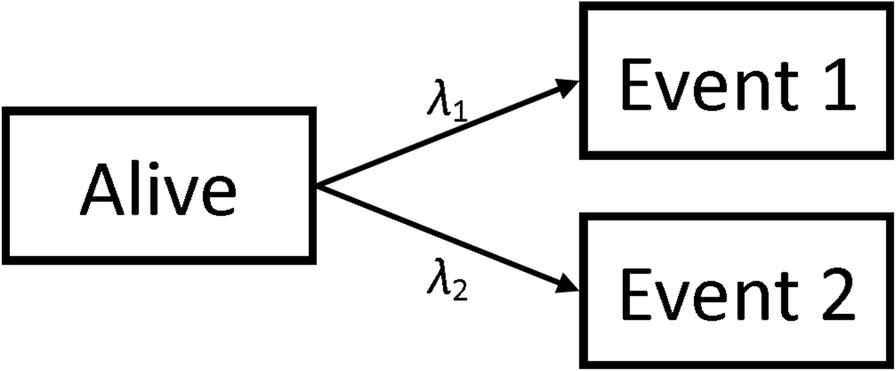
\includegraphics[width=450px]{figure/CR_Conf/Transition_Diagram}

We simulated populations of 10,000 patients to ensure small confidence intervals around our treatment effect estimates in each simulation. Each simulated population had a distinct value for \(\beta\) and \(\gamma\). In order to simulate the confounding of \(U\) and \(Z\), we generated these values such that \(\textrm{Corr}(U,Z) = \rho\) and \(\Pr(Z = 1) = \pi\) {[}19{]}. Population end times and type of event were generated using the relevant hazard functions. The full process for the simulations can be found in Additional file 1. Due to the methods used to generate the populations, the possible values for \(\rho\) are bounded by the choice of \(\pi\) such that when \(\pi = 0.5\), \(\left|\rho\right| <= 0.797\) and when \(\pi = 0.1\) (or \(\pi=0.9\)), \(\left|\rho\right| <= 0.57\). The relationship between the parameters can be seen in the Directed Acyclic Graph (DAG) shown in Fig. @ref(fig:Model\_DAG), where \(T\) is the event time and \(\delta\) is the event type indicator (1 for event-of-interest and 2 for competing event).
\begin{center}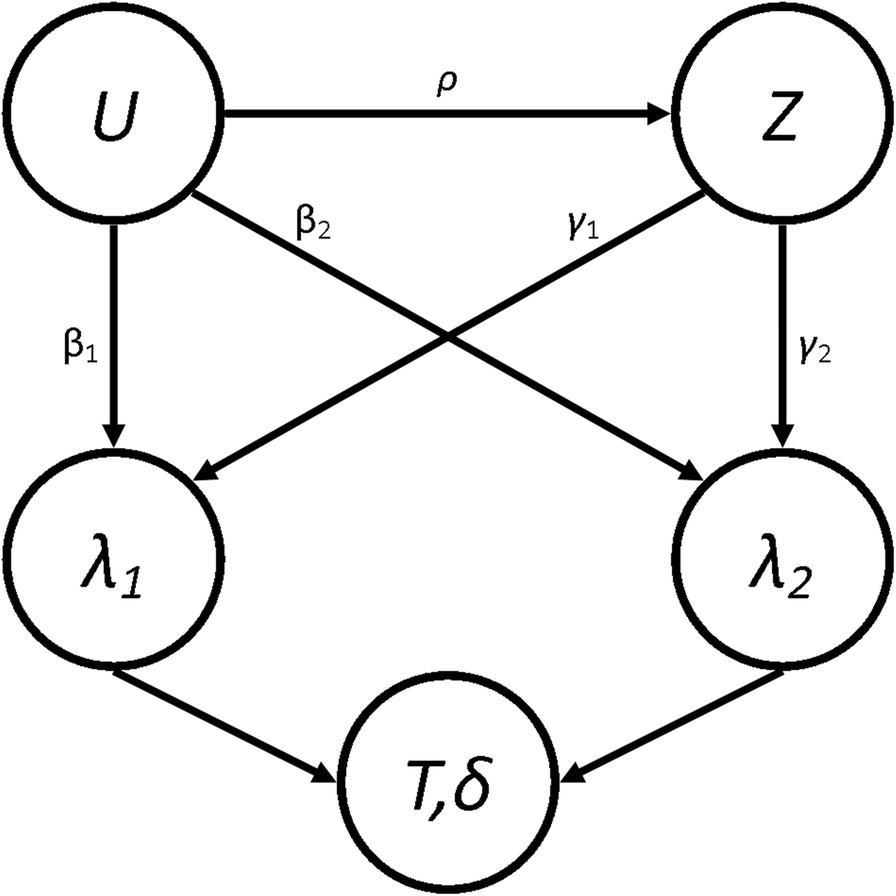
\includegraphics[width=450px]{figure/CR_Conf/DAG} \end{center}

From this, we also explicitly calculated what we would expect the true subdistribution treatment effects, \(\Gamma_1\) and \(\Gamma_2\), to be in these conditions {[}20{]} (See Additional file 2). It's worth noting that the values of \(\Gamma\) will depend on the current value of \(\rho\) since they are calculated using the expected distribution of end-times. However, it has been shown {[}18, 21{]} that, due to the relationship between the Cause-Specific Hazard (CSH) and the Subdistribution Hazard (SH), only one proportional hazards assumption can be true. Therefore the ``true'' values of the \(\Gamma\) will be misspecified and represent a least false parameter (which itself is an estimate of the time-dependent truth) {[}20{]}.

We used the simulated data to estimate the treatment effects under the Cox and Fine \& Gray regression methods. We specify that \(U\) is unmeasured and so it wasn't included in the analysis models. As discussed earlier, the Cox model defines the risk set at time \(t\) to be all patients who have not had any event by time \(t\), whereas the Fine \& Gray defines it to be those who have not had the event-of-interest (or competing event) by time \(t\).

For our models, for the events, \(i={1,2}\), we therefore defined the CSH function estimate, \(\hat{\lambda}_i\), and the SH function estimate, \(\hat{h}_i\), to be

\[
\hat{\lambda}_i(t|Z) = \hat{\lambda}_{i0}(t)e^{\hat{\gamma}_iZ} \qquad\qquad 
\hat{h}_i(t|Z) = \hat{h}_{i0}(t)e^{\hat{\Gamma}_iZ}
\]

Where \(\hat{\lambda}_{i0}(t)\) and \(\hat{h}_{i0}(t)\) are the baseline hazard and baseline subdistribution hazard function estimates for the entire population (i.e.~no stratification), and \(\hat{\gamma}_i\) and \(\hat{\Gamma}_i\) are the estimated treatment effects. From these estimates, we also extracted the estimate of the subdistribution treatment effect in a hypothetical RCT, where \(\rho=0\) and \(\pi=0.5\) to give \(\hat{\Gamma}_{10}\) and \(\hat{\Gamma}_{20}\). To investigate how the correlation between \(U\) and \(Z\) affects the treatment effect estimate, we compared the explicitly prescribed or calculated values with the simulated estimates. Three performance measures for both events, along with appropriate 95\% confidence intervals, were calculated for each set of parameters:
\begin{itemize}
\item
  \(\theta_{\textrm{RCT},i} = \textrm{E}\left[\hat{\Gamma}_i - \hat{\Gamma}_{i0}\right]\) \textasciitilde{} The average difference between the SH treatment effect estimate from an idealised, hypothetical RCT situation.
\item
  \(\theta_{\textrm{Exp},i} = \textrm{E}\left[\hat{\Gamma}_i - \Gamma_i\right]\) \textasciitilde{} The average bias of the SH treatment effect estimate from the explicitly calculated value.
\item
  \(\theta_{\textrm{CSH},i} = \textrm{E}\left[\hat{\gamma}_i - \gamma_i\right]\) \textasciitilde{} The average bias of the CSH treatment effect estimate from the predefined treatment effect.
\end{itemize}
As mentioned above, the value of \(\Gamma\) will depend on the current value of \(\rho\) and so the estimation of the explicit bias will be a measure of the total bias induced on our estimate of the subdistribution treatment effect in those specific set of parameters. We also evaluate the bias compared to an idealised RCT to see how much of this bias could be mitigated if we were to perform an RCT to assess the effectiveness of the hypothetical treatment. Finally, we found the explicit bias in the cause specific treatment effect to again see the total bias applied to this measure. We did not compared the CSH bias to an idealised RCT as we believed that this could easily be inferred from the CSH explicit results, whereas this information wouldn't be as obvious in the SH treatment effect due to the existence of a relationship between \(\Gamma\) and \(\rho\).

Eight Scenarios were simulated based on real-world situations. In each scenario, \(\rho\) varied across 5 different values ranging from 0 to their maximum possible value (0.797 for all Scenarios apart from Scenario 5, where it is 0.57, due to the bounds imposed by the values of \(\pi\)). One other parameter (different for different scenarios) varied across 3 different values, and all other parameters were fixed as detailed in Table 1. Each simulation was run 100 times and the performance measures were each pooled to provide small confidence intervals. This gives a total of 1,500 simulations for each of the 8 scenarios. Descriptions of the different scenarios are given below:
\begin{enumerate}
\def\labelenumi{\arabic{enumi}.}
\item
  No Effect. To investigate whether treatment with no true effect (\(\gamma_2=\gamma_2=0\)) can have an ``artificial'' treatment effect induced on them in the analysis models through the confounding effect on the event-of-interest. \(\beta_1\) varied between -1, 0 and 1.
\item
  Positive Effect. To investigate whether treatment effects can be reversed when the treatment is beneficial for both the event-of-interest and the competing event (\(\gamma_2=\gamma_2=-1\)). \(\beta_1\) varied between -1, 0 and 1.
\item
  Differential Effect. To investigate how treatment effect estimates react when the effect is different for the event-of-interest (\(\gamma_2=-1\)) and the competing event (\(\gamma_2=1\)). \(\beta_1\) varied between -1, 0 and 1.
\item
  Competing Confounder. To investigate whether treatments with no true effect (\(\gamma_1=\gamma_2=0\)) can have an ``artificial'' treatment effect induced on them by the effect of a confounded variable on the competing event only (\(\beta_1=0\)). \(\beta_2\) varied between -1, 0 and 1.
\item
  Uneven Arms. To investigate how having uneven arms on a treatment in the population can have an effect on the treatment effect estimate (\(\gamma_1=-1\), \(\gamma_2=0\)). \(\pi\) varied between \(\sfrac{1}{10}\), \(\sfrac{1}{2}\) and \(\sfrac{9}{10}\).
\item
  Uneven Events. To investigate how events with different frequencies can induce a bias on the treatment effect, despite no treatment effect being present (\(\gamma_1=\gamma_2=0\)). \(k\) varied between \(\sfrac{1}{2}\), \(\sfrac{1}{2}\) and 2.
\item
  Weibull Distribution. To investigate whether a linearly increasing baseline hazard function affects the results found in Scenario 1. \(\beta_1\) varied between -1, 0 and 1.
\item
  Plausible Distribution. To investigate whether a biologically plausible baseline hazard function affects the results found in Scenario 1. \(\beta_1\) varied between -1, 0 and 1.
\end{enumerate}
{[}\textbf{Insert Table 1}{]}

\hypertarget{results-1}{%
\section{Results}\label{results-1}}

The first row of Fig. 3 shows the results for Scenario 1 (No Effect). When \(\beta_1=\beta_2=0\) (the green line), correlation between \(U\) and \(Z\) doesn't imbue any bias on the treatment effect estimate for either event under any of the three measures, since all of the subdistribution treatment effects (estimated, calculated and hypothetical RCT) are approximately zero. When \(\beta_1>0\), there is a strong positive association between correlation (\(\rho\)) and the RCT and CSH biases for the event-of-interest and a negative association for the RCT bias for the competing event. Similarly, these associations are reversed when \(\beta_1<0\).

There was no effect on \(\theta_{\textrm{CSH}}\) for the competing event in this Scenario regardless of \(\rho\) or \(\beta_1\). These results are similar to those found in Scenario 2 (Positive Effect) and Scenario 3 (Negative Effect) shown in Figs. 4 and 5. However, in both of these Scenarios, there is an overall positive shift in \(\theta_{\textrm{CSH}}\) when \(\beta_1\neq0\).

The magnitude of \(\theta_{\textrm{Exp}}\) is greatly reduced and is the reverse of the other associations when \(\beta_1\neq0\) in Scenario 1 for the event-of-interest and when \(\beta_1>0\) it stays extremely small for low values of \(\rho\), and becomes negative for large \(\rho\) for the competing event. In Scenario 2, \(\theta_{\textrm{Exp}}\) behaves similarly to Scenario 1 for both events when \(\beta_1<0\) and the event-of-interest, but for the competing event, when \(\beta_1>0\), the \(\theta_{\textrm{Exp}}\) is much tighter to 0. The competing event data for \(\theta_{\textrm{Exp}}\) in Scenario 3 is similar to Scenario 2 with \(\beta_1>0\) shifted downwards, but the event-of-interest has a near constant level of bias regardless of \(\rho\), apart from in the case when \(\beta_1<0\), the bias switches direction.

In Scenario 4 (Competing Confounder), as would be expected, the results for the event-of-interest and the results for the competing event are swapped from those of Scenario 1 as shown in Fig. 6. Scenario 5 (Uneven Arms) portrays a bias similar to Scenario 1 where \(\beta_1=1\), however, the magnitude of the RCT and CSH bias is increased when \(\pi\neq0.5\) as shown in Fig. 7.

The parameters for Scenario 6 (Uneven Events) were similar to the parameters for Scenario 1 (No Effect), when \(\beta_1=1\). This also reflects in the results in Fig. 8 which look similar to the results for this set of parameters in Scenario 1. This bias is largely unaffected by the value of \(k\). The results of Scenario 7 (Weibull Distribution) and Scenario 8 (Plausible Distribution) were nearly identical to those of Scenario 1 as shown in Figs. 9 and 10.

As per our original hypotheses, Scenario 1 demonstrated that it is possible to induce a treatment effect when one isn't present through confounding effects on all biases, apart from the competing event CSH. In Scenario 2, with high enough correlation, the CSH event-of-interest bias could be greater than 1, meaning that the raw CSH treatment effect was close to 0, despite an actual treatment effect of -1, similarly large positive biases in the SH imply a treatment with no benefit and/or detrimental effect, despite the true treatment being beneficial for both events. This finding is similar for Scenario 3 with large biases changing the direction of the treatment effect (beneficial vs detrimental).

Scenario 4 demonstrated that even without a treatment effect and with no confounding effect on the event-of-interest, a treatment effect can be induced on the SH methodology, which can imply a beneficial/detrimental treatment, depending on whether the confounder was detrimental/beneficial. Fortunately, it does not induce an effect on the CSH treatment effect for the event-of-interest.

Scenarios 5 and 6 investigated other population level effects; differences in the size of the treatment arms and differences in the magnitude of the hazards of the events. Scenario 5 demonstrated that having uneven treatment arms can exacerbate the bias induced on both the \(\theta_{\textrm{RCT}}\) and \(\theta_{\textrm{CSH}}\) for both events and Scenario 6 showed that the different baseline hazards had little effect on the levels of bias in the results. This finding was supported by the additional findings of Scenarios 7 and 8, which showed that the underlying hazard functions did not affect the treatment effect biases compared to a constant hazard.

\hypertarget{discussion}{%
\section{Discussion}\label{discussion}}

This is the first paper to investigate the issue of unmeasured confounding on a treatment effect in a competing risks scenario. Herein, we have demonstrated that regardless of the actual effect of a treatment on a population that is susceptible to competing risks, bias can be induced by the presence of unmeasured confounding. This bias is largely determined by the strength of the confounding relationship with the treatment decision and size of confounding effect on both the event-of-interest and any competing events. This effect is present regardless of any difference in event rates between the events being investigated and is also exacerbated by misbalances in the number of patients who received treatment and the number of patients who did not.

Our study has shown how different the case would be if a similar population (without inclusion/exclusion criteria) were put through an RCT and how the correlation between an unmeasured confounder and the treatment is removed, as would be the case in a pragmatic RCT. By combining the biases from an RCT and the explicitly calculated treatment effect, we can also use these results to infer how much of the bias found here is from omitted variable bias {[}22{]} and how much is explicitly due to the correlation between the covariates. Omitted variable bias occurs when a missing covariate has an effect on the outcome, but is not correlated with the treatment (and so is not a true confounder). It can occur even if the omitted variable is initially evenly distributed between the two treatment arms because, as patients on one arm have events earlier than the other, the distributions of the omitted variable drift apart. This makes up some of the bias caused by unmeasured confounding, but not all of it. For example, in Scenario 3 (Differential Effect), the treatment lowered the hazard of the event-of-interest, but increased the hazard of the competing event; with a median level of correlation (\(\rho=0.4\)), the event-of-interest bias from the RCT when there is a negative confounding effect (\(\beta_1<0\)) is -0.628 and the bias from the explicit estimate is \(0.295\) and therefore, the amount of bias due purely to the correlation between the unmeasured confounder and the treatment is actually -0.923. In this instance, some of the omitted variable bias is actually mitigating the bias from the correlation; if we have two biasing effects that can potentially cancel each other out, we could encounter a Type III error {[}23{]} which is very difficult to prove and can cause huge problems for reproducibility (if you eliminate a single source of bias, your results will be farther from the truth).

Our simulations indicate that a higher (lower) value of \(\beta_1\) and a lower (higher) value of \(\beta_2\) will produce a higher (lower) bias in the event-of-interest. These two biasing effects could cancel out to produce a situation similar to above. In our scenarios, we saw that, even when a treatment has no effect on the event-of-interest or a competing event (i.e.~the treatment is a placebo), both a cause specific treatment effect and a subdistribution treatment effect can be found. This also implies that the biasing effect of unmeasured confounders (both omitted variable and correlation bias) can result in researchers reaching incorrect conclusions about how a treatment affects a population in multiple ways. We could have a treatment that is beneficial for the prevention of both types of event, but due to the effects of an unmeasured confounder, it could be found to have a detrimental effect (for one or both) on patients from a subdistribution perspective.

Our investigation augments Lin et al's study into unmeasured confounding in a Cox model {[}5{]} by extending their conclusion (that bias is in the same direction as the confounder's effect and dependent on its strength) into a competing risks framework (i.e.~by considering the Fine \& Gray model as well) and demonstrating that this effect is reversed when there is confounding with the competing event. Lin et al.~{[}5{]} also highlight the problems of omitted variable bias, which comes from further misspecification of the model; this finding was observed in our results as described above for Scenario 3.

The results from Scenario 7 (Weibull Distribution) and Scenario 8 (Plausible Distribution) are almost identical to those of Scenario 1 (No Effect) which implies that, by assuming both hazard functions in question are the same, we can assume they are both constant for simplicity. Since both the Cox and Fine \& Gray models are ambiguous to underlying hazard functions and treatment effects are estimated without consideration for the baseline hazard function, it makes intuitive sense that the results would be identical regardless of what underlying functions were used to generate our data. This makes calculation of the explicit subdistribution treatment effect much simpler for future researchers.

Thompson et al.~used the paradox that smoking reduces melanoma risk to motivate simulations similar to ours, which demonstrated how the exclusion of competing risks, when assessing confounding, can lead to unintuitive, mis-specified and possibly dangerous conclusions {[}24{]}. They hypothesised that the association found elsewhere {[}25{]} may be caused by bias due to ignoring competing events and used Monte Carlo simulations to provide examples of scenarios where these results would be possible. They demonstrated how a competing event could cause incorrect conclusions when that competing event is ignored - a conclusion we also confirm through the existence of bias induced on the Cox modelled treatment effect even with no correlation between the unmeasured confounder and treatment (i.e.~\(\theta_{\textrm{CSH,1}} \neq 0\) in Scenarios 2 \& 3). Thompson's team began with a situation where there may be a bias due to a competing event and reverse-engineered a scenario to find the potential sources of bias, whereas our study explored different scenarios and investigated the biased results they potentially produced.

Groenwold et al.~{[}26{]} proposed methods to perform simulations to evaluate how much unmeasured confounding would be necessary for a true effect to be null given that an effect has been found in the data. Their methods can easily be applied to any metric in clinical studies (such as the different hazard ratios estimated here). Currently, epidemiologists will instigate methods such as DAGs, see Fig. @ref(fig:Model\_DAG), to visualise where unmeasured confounding may be a problem in analysis {[}27{]} and statisticians who deal with such models will use transition diagrams, see Fig. @ref(fig:Model\_Transitions), to visualise potential patient pathways {[}28{]}. Using these two visualisation techniques in parallel will allow researchers to anticipate these issues, successfully plan to combat them (through changes to protocol or sensitivity analysis, etc. \ldots) and/or implement simulations to seek hidden sources of bias (using the methods of Groenwold {[}26{]} and Thompson {[}24{]}) or to adjust their findings by assuming biases similar to those demonstrated in our paper exist in their work.

The work presented here could be extended to include more complicated designs such as more competing events, more covariates and differing hazard functions. However, the intention of this paper was to provide a simple dissection of specific scenarios that allow for generalisation to clinical work. The main limitation of this work, to use of the same hazard functions for both events in each of our scenarios, was a pragmatic decision made to reduce computation time. The next largest limitation was the lack of censoring events, and was chosen to simplify interpretation of the model. This situation is unlikely to happen in the real world. However, since both the Cox and the Fine \& Gray modelling techniques are robust to any underlying baseline hazard and independent censoring of patients {[}14, 15, 29{]}, these simplifications should not have had a detrimental effect on the bias estimates given in this paper. This perspective on censoring is similar to the view of Lesko et al.~{[}30{]} in that censoring would provide less clarity of the presented results.

\hypertarget{conclusion-1}{%
\section{Conclusion}\label{conclusion-1}}

This paper has demonstrated that unmeasured confounding in observational studies can have an effect on the accuracy of outcomes for both a Cox and a Fine \& Gray model. We have added to the literature by incorporating the effect of confounding on a competing event as well as on the event-of-interest simultaneously. The effect of confounding is present and reversed compared to that of confounding on the event-of-interest. This makes intuitive sense as a negative effect on a competing event has a similar effect at the population level as a positive effect on the event-of-interest (and vice versa). This should not be overlooked, even when dealing with populations where the potential for competing events is much smaller than potential for the event-of-interest and is especially true when the two arms of a study are unequal. Therefore, we recommend that research with the potential to suffer from these issues be accompanied by sensitivity analyses investigating potential unmeasured confounding using established epidemiological techniques applied to any competing events as well as the event-of-interest. In short, unmeasured variables can cause problems with research, but by being knowledgeable about what we don't know, we can make inferences despite this missing data.

\hypertarget{chap-IPCW-logistic}{%
\chapter{Inverse Probability Weighting Adjustment of the Logistic Regression Calibration-in-the-Large}\label{chap-IPCW-logistic}}

\emph{MA Barrowman, A Pate, GP Martin, CJM Sammut-Powell, M Sperrin}
\chaptermark{IPCW Calibration-in-the-Large}
Last updated: 03 May

\hypertarget{abstract-1}{%
\section*{Abstract}\label{abstract-1}}
\addcontentsline{toc}{section}{Abstract}

\hypertarget{introduction-3}{%
\subsection*{Introduction}\label{introduction-3}}
\addcontentsline{toc}{subsection}{Introduction}

\hypertarget{methods-3}{%
\subsection*{Methods}\label{methods-3}}
\addcontentsline{toc}{subsection}{Methods}

\hypertarget{results-2}{%
\subsection*{Results}\label{results-2}}
\addcontentsline{toc}{subsection}{Results}

\hypertarget{discussion-1}{%
\subsection*{Discussion}\label{discussion-1}}
\addcontentsline{toc}{subsection}{Discussion}

\hypertarget{supplementary-material-1}{%
\subsection*{Supplementary Material}\label{supplementary-material-1}}
\addcontentsline{toc}{subsection}{Supplementary Material}

Supplementary Material is available in Appendix \ref{chap-dev-paper-supp}.

\hypertarget{introduction-4}{%
\section{Introduction}\label{introduction-4}}

\sout{Clinical prediction models (CPMs)}Clinical prediction models (CPMs) are statistical models/algorithms that aim to predict the presence (diagnostic) or furture occurence (prognostic) of an event of interest, conditional on a set of predictor variables. Before they be implemented in practice, CPMs must be robustly validated. They need to be validated before they are used and a\sout{A} fundamental test of their validity is calibration: the agreement between observed and predicted outcomes. This requires that among individuals with \(p\%\) risk of an event, \(p\%\) of those have the event across the full risk range {[}\protect\hyperlink{ref-steyerberg_clinical_2008}{35}{]}. The simplest assessment of calibration is the calibration-in-the-large, which tests for agreement in mean calibration (the weakest form of calibration) {[}\protect\hyperlink{ref-calster_calibration_2016-1}{36}{]}. With continuous or binary outcomes, such a test is straight-forward: it can be translated to a test for a zero intercept in a regression model with an appropriately transformed linear predictor as an offset, and no other predictors. More complicated measurements of calibration can also be assessed to descibe how calibration changes across the risk range, such as calibration slope (see Appendix \ref{chap-IPCW-logistic-supp}). Calibration alone is not enough to fully assess a model's performance however and so we also need measures of discrimination (how well models discern between different patients), e.g the c-statistic and overall accuracy, e.g.~the Brier Score.

\sout{In the case of Cox regression, however, estimation of calibration is complicated in three ways. First, calibration can be computed at multiple time-points and one must decide which time-points to evaluate, and how to integrate over these time-points. Second, there exists no explicit intercept in the model because of the non-parametric baseline hazard function {[}\protect\hyperlink{ref-royston_external_2013}{37}{]}. Third, censoring needs to be handled in an appropriate way. The choice and combination of time-points determines what we mean by calibration; this is problem-specific and not the focus of this paper. Calibration can also be looked at integrated over time using martingale residuals {[}\protect\hyperlink{ref-crowson_assessing_2016}{38}{]}; however here we focus on the case where calibration at a specific time point is of interest - e.g.~as is common in clinical decision support. The lack of intercept can be overcome provided sufficient information concerning the baseline survival curve is available (although this is rarely the case {[}\protect\hyperlink{ref-houwelingen_validation_2000}{39}{]}. Once this is established, estimated survival probabilities are available. Censoring leads to problems in determining observed survival. This is commonly overcome by using Kaplan-Meier estimates {[}\protect\hyperlink{ref-hippisley-cox_derivation_2007}{27}{]}, {[}\protect\hyperlink{ref-royston_external_2013}{37}{]}. However the censoring assumptions required for the Kaplan-Meier estimate are stronger than those required for the Cox model: the former requiring unconditional independence (random censoring), the latter requiring independence conditional on covariates only. This is a problem because when miscalibration is found using this approach, it is not clear whether this is genuine miscalibration or a consequence of the different censoring assumptions.}

\sout{Royston {[}\protect\hyperlink{ref-royston_tools_2014}{40}{]} presents an alternative approach for calibration at external validation. He uses the approach of pseudo-observations, as described by Perme and Anderson {[}\protect\hyperlink{ref-perme_checking_2008}{41}{]} to overcome the censoring issue and produce observed probabilities at individual level; however, this assumes that censoring is independent of covariates. In this paper and another {[}\protect\hyperlink{ref-royston_tools_2015}{42}{]} he proposes the comparison of KM curves in risk groups, which alleviates the strength of the independence assumption required for the censoring handling to be comparable between the Cox model and the KM curves (since the KM curves now only assume independent censoring within risk group). In these papers a fractional polynomial approach to estimating the baseline survival function (and thus being able to share it efficiently) is also provided.}

In the case of time to event models, however, estimation of calibration is complicated in three ways. First, calibration can be computed at multiple time-points and one must decide which time-points to evaluate, and how to integrate over these time-points. The choice and combination of time-points determines what we mean by calibration; this is problem-specific and not the focus of this paper. Calibration can also be integrated over time using the martingale residuals {[}\protect\hyperlink{ref-crowson_assessing_2016}{38}{]}; however we focus on the case where calibration at a specific time point is of interest - e.g.~as is common in clinical decision support. Second, there exists no explicit intercept in the model because of the non-parametric baseline hazard function {[}\protect\hyperlink{ref-royston_external_2013}{37}{]}. The lack of intercept can be overcome provided sufficient information concerning the baseline survival curve is available (although this is rarely the case as seen in QRISK{[}\textbf{Cite: }{]}, ASCVD{[}\textbf{Cite: }{]} and ASSIGN{[}\textbf{Cite: }{]}. Once this is established, estimated survival probabilities are available.

Third, censoring needs to be handled in an appropriate way. This is commonly overcome by using Kaplan-Meier estimates {[}\protect\hyperlink{ref-hippisley-cox_derivation_2007}{27}{]}, {[}\protect\hyperlink{ref-royston_external_2013}{37}{]}, but the censoring assumptions required for the Kaplan-Meier estimate are stronger than those required for the Cox model: the former requiring unconditional independence (random censoring), the latter requiring independence conditional on covariates only. This is a problem because when miscalibration is found using this approach, it is not clear whether this is genuine miscalibration or a consequence of the different censoring assumptions. Royston {[}\protect\hyperlink{ref-royston_tools_2014}{40}{]}, {[}\protect\hyperlink{ref-royston_tools_2015}{42}{]} has proposed the comparison of KM curves within risk groups, which alleviates the strength of the independence assumption required for the censoring handling to be comparable between the Cox model and the KM curves (since the KM curves now only assume independent censoring within risk group). In these papers a fractional polynomial approach to estimating the baseline survival function (and thus being able to share it efficiently) is also provided. However, this does not allow calculations of the overall calibration of the model, which is of primary interest here.

QRISK used the overall KM approach in the 2007 paper {[}\protect\hyperlink{ref-hippisley-cox_derivation_2007}{27}{]} with good results (6.34\% predicted vs 6.25\% observed in women and 8.86\% predicted vs 8.88\% observed in men), but \sout{bad}worse results in the QRISK3 update {[}\protect\hyperlink{ref-hippisley-cox_development_2017}{2}{]} (4.7\% predicted v 5.8\% observed in women and 6.4\% predicted vs 7.5\% observed in men ). This may be because, as follow-up extends, the dependence of censoring on the covariates increases (QRISK had 12 years follow-up, QRISK3 had 18) and an important change between the update was the lower age limit moved from 35 to 25, as well as the implementation of QRISK in clinical practice {[}\textbf{I remember discussing this with Alex \& Matt a while ago as to whether the use of QRISK had a feedback loop when updated after it's own implementation. Did this go any further?}{]}.

Royston {[}\protect\hyperlink{ref-royston_tools_2014}{40}{]} also presented an alternative approach for calibration at external validation. He uses the approach of pseudo-observations, as described by Perme and Anderson {[}\protect\hyperlink{ref-perme_checking_2008}{41}{]} to overcome the censoring issue and produce observed probabilities at individual level; however, this assumes that censoring is independent of covariates.

A solution to this problem is to apply a weighting to uncensored patients based on their probability of being censored according to a model that accounts for covariates. The Inverse Probability of Censoring Weighting (IPCW) relaxes the assumption that patients who were censored are identical to those that remain at risk and replaces it with the assumption that they are exchangeable conditional on the measured covariates. The weighting inflates the patients who were similar to the censored population to account for those patients who are no longer available at a given time.

Gerds \& Schumacher {[}\protect\hyperlink{ref-gerds_consistent_2006}{43}{]} have thoroughly investigated the requirements and advantages of applying an IPCW to a performance measure for modelling using the Brier score as an example and demonstrating the efficacy of its use, which was augmented by Spitoni et al {[}\protect\hyperlink{ref-spitoni_prediction_2018}{44}{]} who demonstrated that any proper scoring rule can be improved by the use of the IPCW. This work has been \sout{added to}extended by Han et al {[}\protect\hyperlink{ref-han_comparing_2017}{45}{]} and Liu et al {[}\protect\hyperlink{ref-liu_comparing_2016}{46}{]} who demonstrated \sout{that the c-statistic is also suitable}one can also apply IPCW to the c-statistic (a measure of discrimination).

In this paper we present an approach to assessing the calibration intercept (calibration-in-the-large) and calibration slope in time-to-event models based on estimating the censoring distribution, and reweighting observations by the inverse of the censoring probability. We first show, theoretically, how this method can be used and evidence that the metrics for calibration are amenable to its use. We then compare simulation results from using this weighted estimate to an unweighted estimate within various commonly used methods of calibration assessment.

\hypertarget{methods-4}{%
\section{Methods}\label{methods-4}}

\hypertarget{theory}{%
\subsection{Theory}\label{theory}}

{[}\textbf{Lots of Theory work on the probabilities. May need to drop this if we're unable to do it between us.}{]}

\hypertarget{aims}{%
\subsection{Aims}\label{aims}}

The aim of this simulation study is to \sout{formalise}investigate the bias induced by applying different methods of assessing model calibration to data that is susceptible to censoring and to compare it to the bias when this data has been adjusted by the Inverse Probability of Censoring Weighting (IPCW).

\hypertarget{data-generating-method}{%
\subsection{Data Generating Method}\label{data-generating-method}}

We simulated populations of patients with survival and censoring times, and took the observed event time as the minimum of these two values along with an event indicator of whether this was the survival or censoring time {[}\protect\hyperlink{ref-burton_design_2006}{47}{]}. Each population was simulated with \sout{two}three parameters: \(\beta\), \(\gamma\) and \(\eta\), which defined the proportional hazards coefficients for the survival and censoring distributions and the baseline hazard function, respectively.

\sout{We varied the parameters to take all the values,\(\gamma = \{-2,-1.5,-1,-0.5,0,0.5,1,1.5,2\}\), \(\beta = \{-2,-1.5,-1,-0.5,0.5,1,1.5,2\}\) and \(\eta = \{-\sfrac{1}{2},0,\sfrac{1}{2}\}\), that is the proportional hazard coefficients took the same values between -2 and 2, but \(\beta\) did not take the value of 0 because this would make a predictive model infeasible.}

\sout{For each combination of parameters, we generated \(N = 100\) populations of \(n = 10,000\) patients (a high number of patients was chosen to avoid bias due to a small population sizeimprove precision of our estimates with}Patients were generated with a single covariate \(Z \sim N(0,1)\)\sout{. For each patient,} from which, we then generated a survival time, \(T\) and a censoring time, \(C\). Survival times were simulated with a baseline hazard \(\lambda_0(t) = t^{\eta}\) (i.e.~Weibull), and a proportional hazard of \(e^{\beta Z}\). This allows the simulation of a constant baseline hazard (\(\eta = 0\)) as well as an increasing (\(\eta = \sfrac{1}{2}\)) and decreasing (\(\eta = -\sfrac{1}{2}\)) hazard function Censoring times were simulated with a constant baseline hazard, \(\lambda_{C,0}(t) = 1\) and a proportional hazard of \(e^{\gamma Z}\). This combines to give a simulated survival function, \(S\) as
\[
S(t|Z=z) = \exp\left(-\frac{e^{\beta Z}t^{\eta+1}}{\eta+1}\right)
\]
and a simulated censoring function, \(S_c\) as
\[
S_c(t|Z=z) = \exp\left(-e^{\gamma Z}t\right)
\]

Once the survival and censoring times were generated, the event time, \(X = \min(T,C)\), and the event indicator, \(\delta = I(T=X)\), were generated. In \sout{the real-world}practice, only \(Z\), \(X\) and \(\delta\) would be observed.

\sout{For each population, a prediction model for survival, \(F_P\) was chosen to be identical to the Data Generating Mechanism (DGM) to emulate a perfectly calibrated model (\ldots)}

\sout{This prediction model was used to generate an estimate of the Expected probability that a given patient, with covariate \(z\), will have an event at the given time. To test the ability of approaches to detect miscalibration, we also derived a prediction model that would systematically over-estimate the prediction model, \(F_O\) and one which would systematically under-estimate the prediction, \(F_U\). These are defined as such (\ldots)}

\sout{The prediction models were assessed at 100 time points, evenly distributed between the 25th and 75th percentile of observed event times, \(X\). At each time point, \(t\), we removed patients who had been censored (i.e.~\(T < X_i\) \& \(\delta_i = 0\)) and created an indicator variable for whether each patient had had the event yet or not: (\ldots)}

\sout{Similarly, we calculate a censoring prediction model, \(G\), to be identical to the DGM: (\ldots)}

\sout{This is used to calculate an IPCW for all non-censored patients at the last time they were observed (\(t\) for patients who have not had an event, and \(X_i\) for patients who have had the event), This is defined as:(\ldots)}

During each simulation, we varied the parameters to take all the values,\(\gamma = \{-2,-1.5,-1,-0.5,0,0.5,1,1.5,2\}\), \(\beta = \{-2,-1.5,-1,-0.5,0,0.5,1,1.5,2\}\) and \(\eta = \{-\sfrac{1}{2},0,\sfrac{1}{2}\}\). For each combination of parameters, we generated \(N = 100\) populations of \(n = 10,000\) patients (a high number of patients was chosen to improve precision of our estimates)

\hypertarget{prediction-models}{%
\subsection{Prediction Models}\label{prediction-models}}

{[}\textbf{New section, taken from previous snippets, highlighting/strikethroughs will show the new changes}{]}

For each population, we used three distinct prediction models \sout{a prediction model} for survival. \(F_P\) was chosen to exactly model the Data Generating Mechanism (DGM) to emulate a perfectly \sout{calibrated}specified model:

\[
\begin{array}{c}
F_P(t|Z = z) = 1 - \exp\left(-\frac{e^{\beta Z}t^{\eta+1}}{\eta+1}\right)
\end{array}
\]
From this, we also derived a prediction model that would systematically over-estimate the prediction model, \(F_O\), and one which would systematically under-estimate the prediction, \(F_U\). These are defined as:

\[
\begin{array}{rl}
F_U(t|Z=z) =& \logit^{-1}\left(\logit\left( F_P(t|z) - 0.2\right)\right)
\end{array}
\]
\[
\begin{array}{rl}
F_O(t|Z=z) =& \logit^{-1}\left(\logit\left( F_P(t|z) + 0.2\right)\right)
\end{array}
\]

\sout{This}These prediction models \sout{was}were used to generate an estimate of the Expected probability that a given patient, with covariate \(z\), will have an event at the given time.

\hypertarget{the-ipcw}{%
\subsection{The IPCW}\label{the-ipcw}}

In order to apply the IPCW, we need to\sout{Similarly, we} calculate a censoring prediction model. For our purposes, we will again use a perfectly specified censoring distribution, \(G\), to be derived directly from\sout{identical to} the DGM:

\[
\begin{array}{c}
G(t|Z=z) = 1-\exp\left(-e^{\gamma Z}t\right)
\end{array}
\]
This is used to calculate an IPCW for all non-censored patients at the last time they were observed (\(t\) for patients who have not had an event, and \(X_i\) for patients who have had the event), This is defined as:

\[
\begin{array}{c}
\omega(t|z) = \frac{1}{1 - G(\min(t,X_i)|z)}
\end{array}
\]

\hypertarget{calibration-measurements}{%
\subsection{Calibration Measurements}\label{calibration-measurements}}

The prediction models were assessed at 100 time points, evenly distributed between the 25th and 75th percentile of observed event times, \(X\). At each of these time points, we compare Observed outcomes (\(O\)) with the Expected outcomes (\(E\)) of the prediction models based on four choices of methodology {[}\protect\hyperlink{ref-riley_prognosis_2019}{6}{]}, {[}\protect\hyperlink{ref-royston_tools_2014}{40}{]}, {[}\protect\hyperlink{ref-royston_tools_2015}{42}{]}, {[}\protect\hyperlink{ref-andersen_pseudo-observations_2010}{48}{]} to produce measures for the calibration-in-the-large
\begin{itemize}
\tightlist
\item
  Kaplan-Meier (KM) - A Kaplan-Meier estimate of survival is estimated from the data and the value of the KM curve at the current time is taken to be the average Observed number of events within the population and this is compared with the average Expected value.
\item
  Logistic Unweighted (LU) - Logistic regression is performed on the non-censored population to predict the binary Observed value using the logit(Expected) value as an offset and the Intercept of the regression is the estimate of calibration-in-the-large.
\item
  Logistic Weighted (LW) - As above, but the logistic regression is performed using the IPCW as a weighting for each non-censored patient.
\item
  Pseudo-Observations (PO) - The contribution of each patient (including censored patients) to the overall Observed value is calculated by removing them from the population and aggregating the difference. \sout{Logistic r}Regression is performed \sout{using}with the complimentary log-log function as a link function and the log cumulative hazard as an offset \sout{and}with the Intercept \sout{of the result is the estimate}representing the estimate of calibration-in-the-large.
\end{itemize}
\sout{The weights within the LW method create a non-integer number of events within the regression. and the PO method can produce values that are not always 0 or 1 (as would be expected in an ordinary logistic regression). The values produced by PO will have to be artificially capped between 0 and 1, but otherwise these two methods do not cause any issues.}Some of these methods produce unusual results for the regressions. Firstly, the weights within the LW method cause the ``number of events'' being processed (i.e the sum of the weighted events) to be non-integer. This is a minor issue and can be dealt with by most software packages {[}\protect\hyperlink{ref-wildscop_biostatistics_2013}{49}{]}. Secondly, the PO method produces outcomes that are outside of the (0,1) range {[}\protect\hyperlink{ref-perme_checking_2008}{41}{]} required for the complimentary log-log function. To combat this, we re-scale the values produced to be with this range and perform the regression as normal.

\hypertarget{estimands}{%
\subsection{Estimands}\label{estimands}}

For each set of parameters and methodology, our estimand at time, \(t\), measured in simulation \(i = 1,...,N\) is \(\theta_i(t)\), the set of estimates of the calibration-in-the-large for the \(F_P\), \(F_U\) and \(F_O\) models in order. Therefore our underlying truth for all time points is

\[\begin{array}{c}
\theta = \left(0,0.2,-0.2\right)
\end{array}\]
From this, we can also define our upper and lower bound for a 95\% confidence interval as the vectors \(\theta_{i,L}(t)\) and \(\theta_{i,U}(t)\).

\hypertarget{performance-measures}{%
\subsection{Performance Measures}\label{performance-measures}}

The measures we will take as performance measures as the Bias, the Empirical Standard Error \sout{as}and the Coverage at time, \(t\), along with relevant standard errors and confidence intervals as per current recommendations {[}\protect\hyperlink{ref-morris_using_2019}{50}{]}. These measures can be seen in table \ref{tab:PM-DGM-time}. For these estimates at each time point, Method and Model, the top and bottom 5\% of all simulation estimates will be omitted, leaving \(N=90\) to avoid biasing the results from singly large random effects.
\begin{table}

\caption{\label{tab:PM-DGM-time}{\small Performance Measures to be taken at each time point}}
\centering
\fontsize{7}{9}\selectfont
\begin{tabular}[t]{lll}
\toprule
Performance Measure & Estimation & SE\\
\midrule
\rowcolor{gray!6}  Bias & $\hat{\theta}(t) = \frac{1}{N} \sum_{i=1}^N\theta_i(t) - \theta$ & $\hat{\theta}_{SE}(t) = \sqrt{\frac{1}{N(N-1)} \sum_{i=1}^N \left(\theta_i(t) - \hat{\theta}(t)\right)^2}$\\
EmpSE & $\hat{E}(t) = \sqrt{\frac{1}{N-1}\sum_{i=1}^N\left(\theta_i(t) - \hat{\theta}(t)\right)^2}$ & $\hat{E}_{SE}(t)=\frac{\hat{E}(t)}{\sqrt{2(N-1)}}$\\
\rowcolor{gray!6}  Coverage & $\hat{C}(t)=\frac{1}{N}\sum_{i=1}^NI\left(\theta_{i,L}(t) \le \theta \le \theta_{i,U}(t)\right)$ & $\hat{C}_{SE}(t) = \frac{\hat{C}(t)\left(1-\hat{C}(t)\right)}{N}$\\
\bottomrule
\end{tabular}
\end{table}
The bias provides a measure of how close our estimate is to the true value as per our data generating mechanisms. The coverage will demonstrate how often our confidence intervals surrounding our estimate actually include this true value. The Empirical Standard Error will show us how precise our estimates are.

\sout{For each estimand above, \(\hat{Q}(t) = \{\hat{\theta}(t),\hat{E}(t), \hat{C}(t)\}\) and associated SE, \(\hat{Q}_\textrm{SE}(t) = \{\hat{\theta}_\textrm{SE}(t),\hat{E}_\textrm{SE}(t), \hat{C}_\textrm{SE}(t)\}\), we average over time. As these measures will be taken at each of the 100 time points, \(t_j:j=1...100\), we summarise each of these measures as an average and as weighted average, as seen in table \ref{tab:PM-DGM}. The weight used for the measure at time \(t_j\) is the average number of non-censored patients remaining in the population at time \(t_j\), defined as \(n_j\) (note that this includes patients who have had the event).(\ldots)}

\hypertarget{software}{%
\subsection{Software}\label{software}}

All analysis was done in \texttt{R\ 3.6.3} {[}\protect\hyperlink{ref-r_core_team_r_nodate}{51}{]} using the various \texttt{tidyverse} packages {[}\protect\hyperlink{ref-wickham_tidy_2017}{52}{]}, Kaplan-Meier estimates were found using the \texttt{survival} package {[}\protect\hyperlink{ref-therneau_package_2020}{53}{]}, Pseudo-Observations were evaluated with the \texttt{pseudo} package {[}\protect\hyperlink{ref-perme_pseudo_2017}{54}{]}, and the results app was developed using \texttt{shiny}{[}\protect\hyperlink{ref-chang_shiny_2020}{55}{]}. The code used for this simulation study is available \href{https://github.com/MyKo101/IPCW-Logistic}{on Github} and the results can be seen in a \href{https://michael-barrowman.shinyapps.io/IPCW_Calibrations/?_ga=2.129261196.1072091615.1588464259-38998367.1584541320}{shiny app}

\hypertarget{results-3}{%
\section{Results}\label{results-3}}

{[}\textbf{Results shown here are new and improved from the previous version. No highlighting is shown}{]}
\begin{figure}
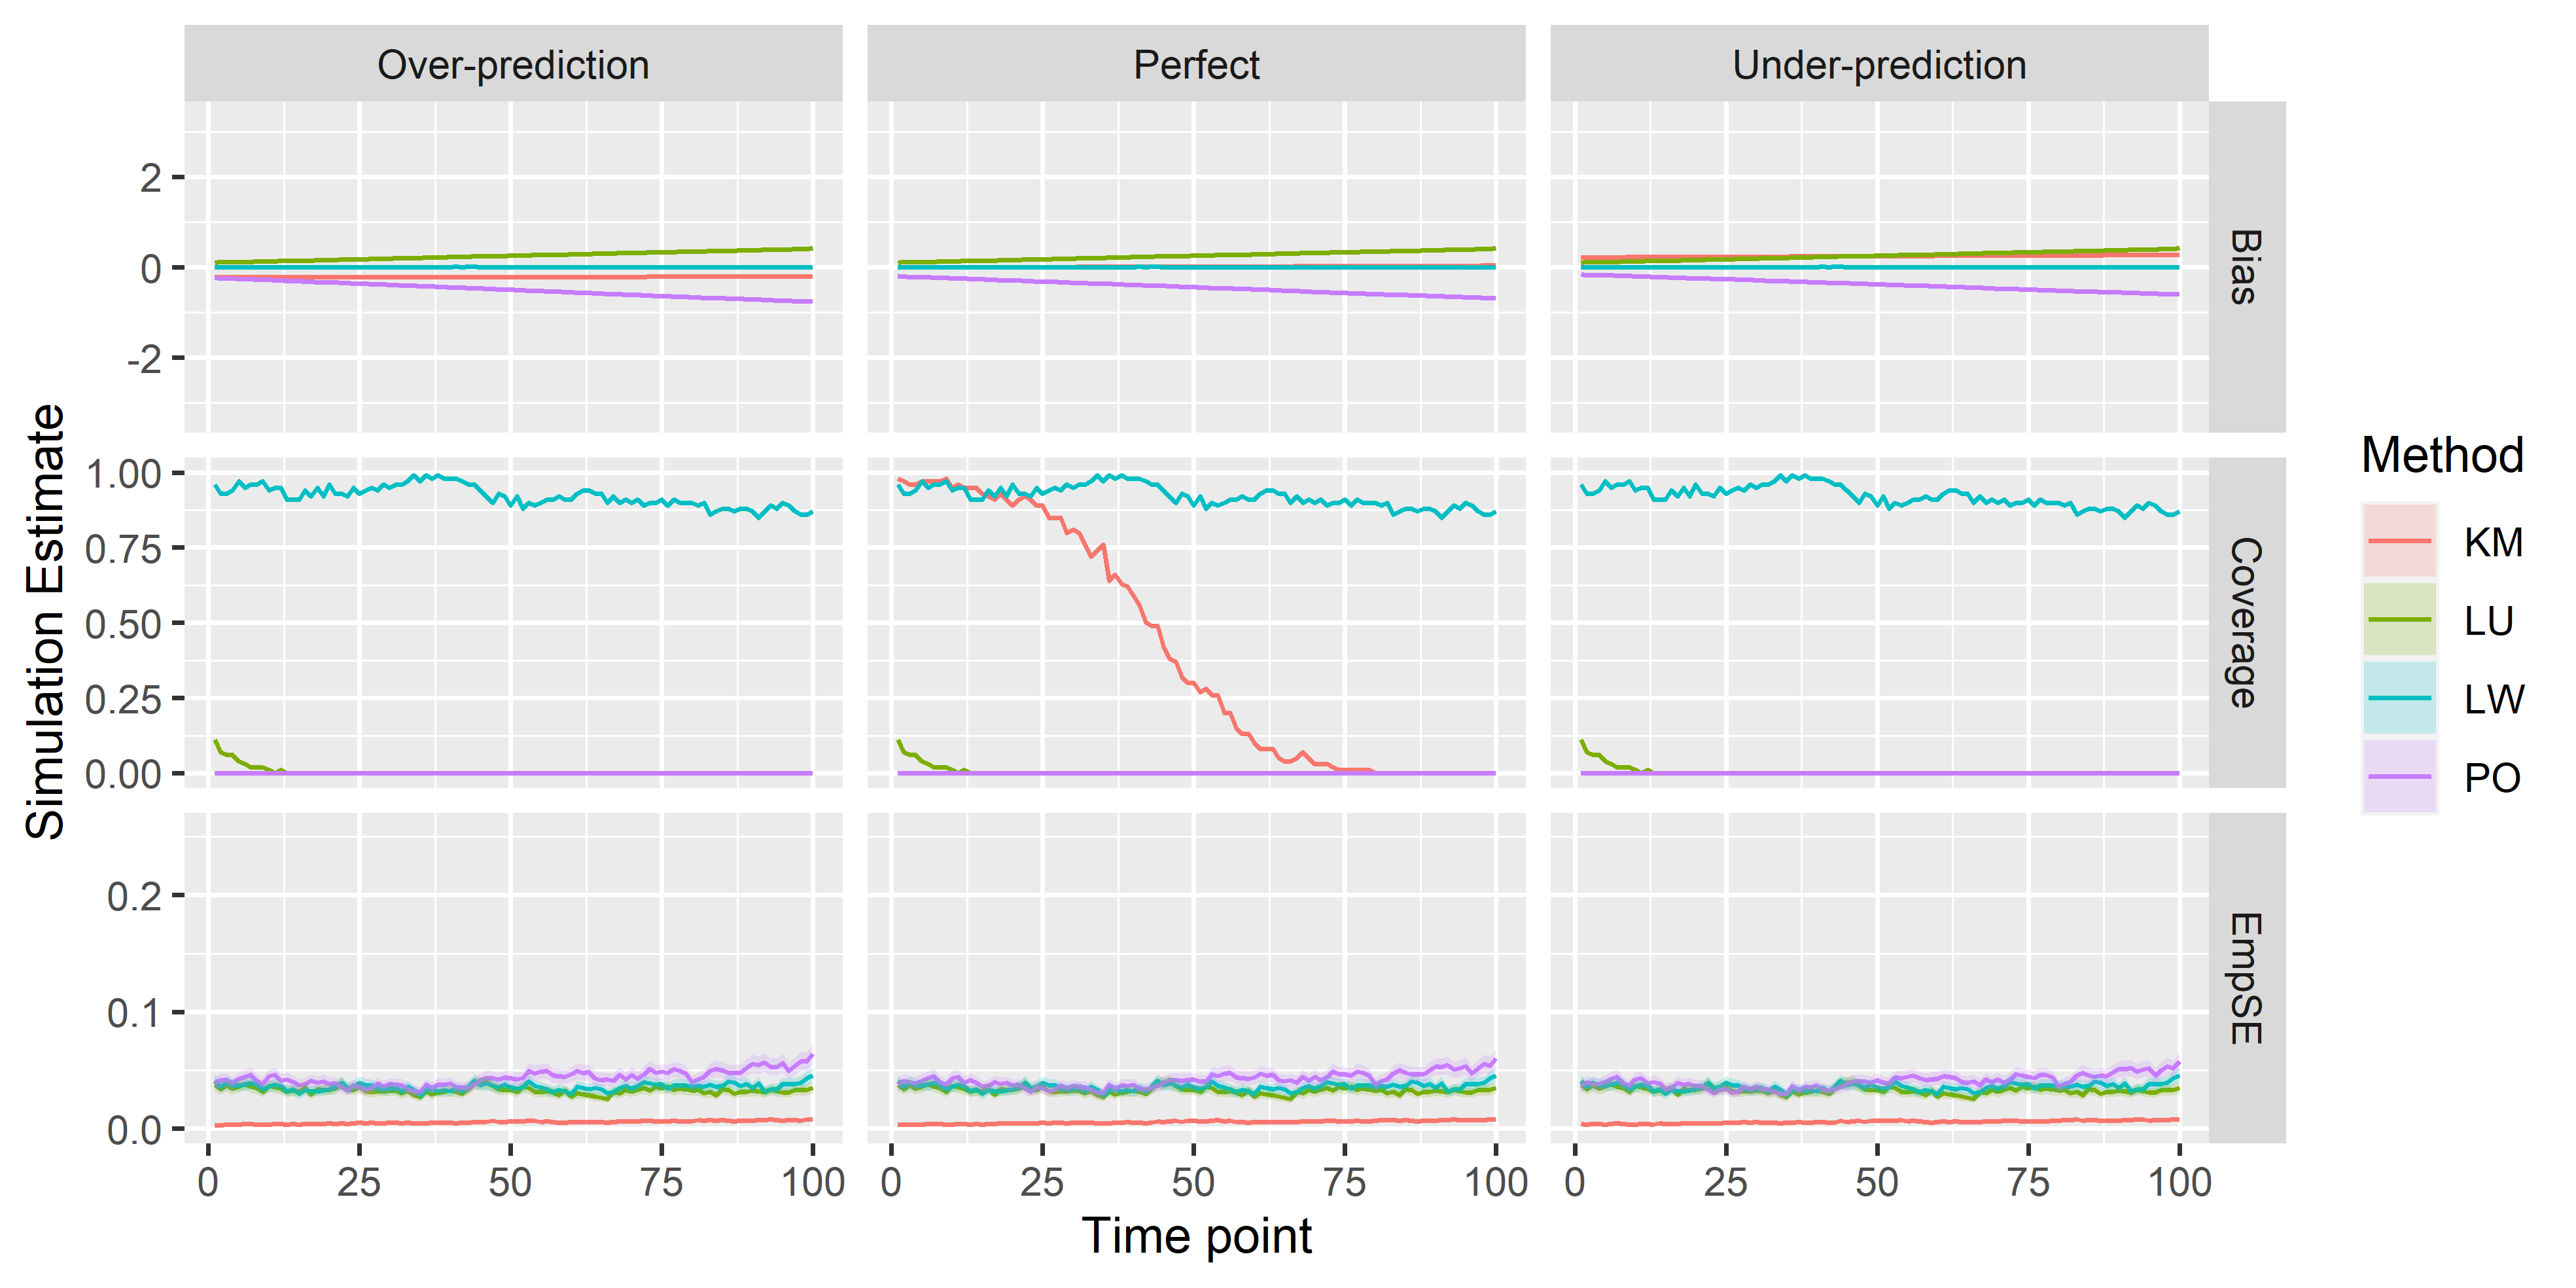
\includegraphics[width=54.68in]{figure/IPCW_Logistic/MainPlot_b(1)_g(0)_e(0.5)} \caption{Bias, Coverage and Empirical Standard Error for the Over-estimating, Perfect and Under-Estimating models across all four methods when $\beta=1$, $\gamma=0$ and $\eta=\sfrac{1}{2}$. Confidence Intervals are included in the plot, but are tight around the estimate}\label{fig:MainPlotg0}
\end{figure}
Figure \ref{fig:MainPlotg0} shows the results when censoring is independent of covariates (\(\gamma=0\)). The LW method provides strong coverage across the entire timeframe and miminal bias. The absolute bias for PO and LU increases over time with PO under-reporting the correct value and LO over-reporting. KM bias remains constant across the timeframe, but for the imperfect models, is constantly under- or over-reported. LU and PO also provide minimal coverage at all time points, whereas KM covers perfect in the early stages of the Perfect Model with coverage dropping off as time progresses. Empirical Standard Error is clse to 0 for all models.
\begin{figure}
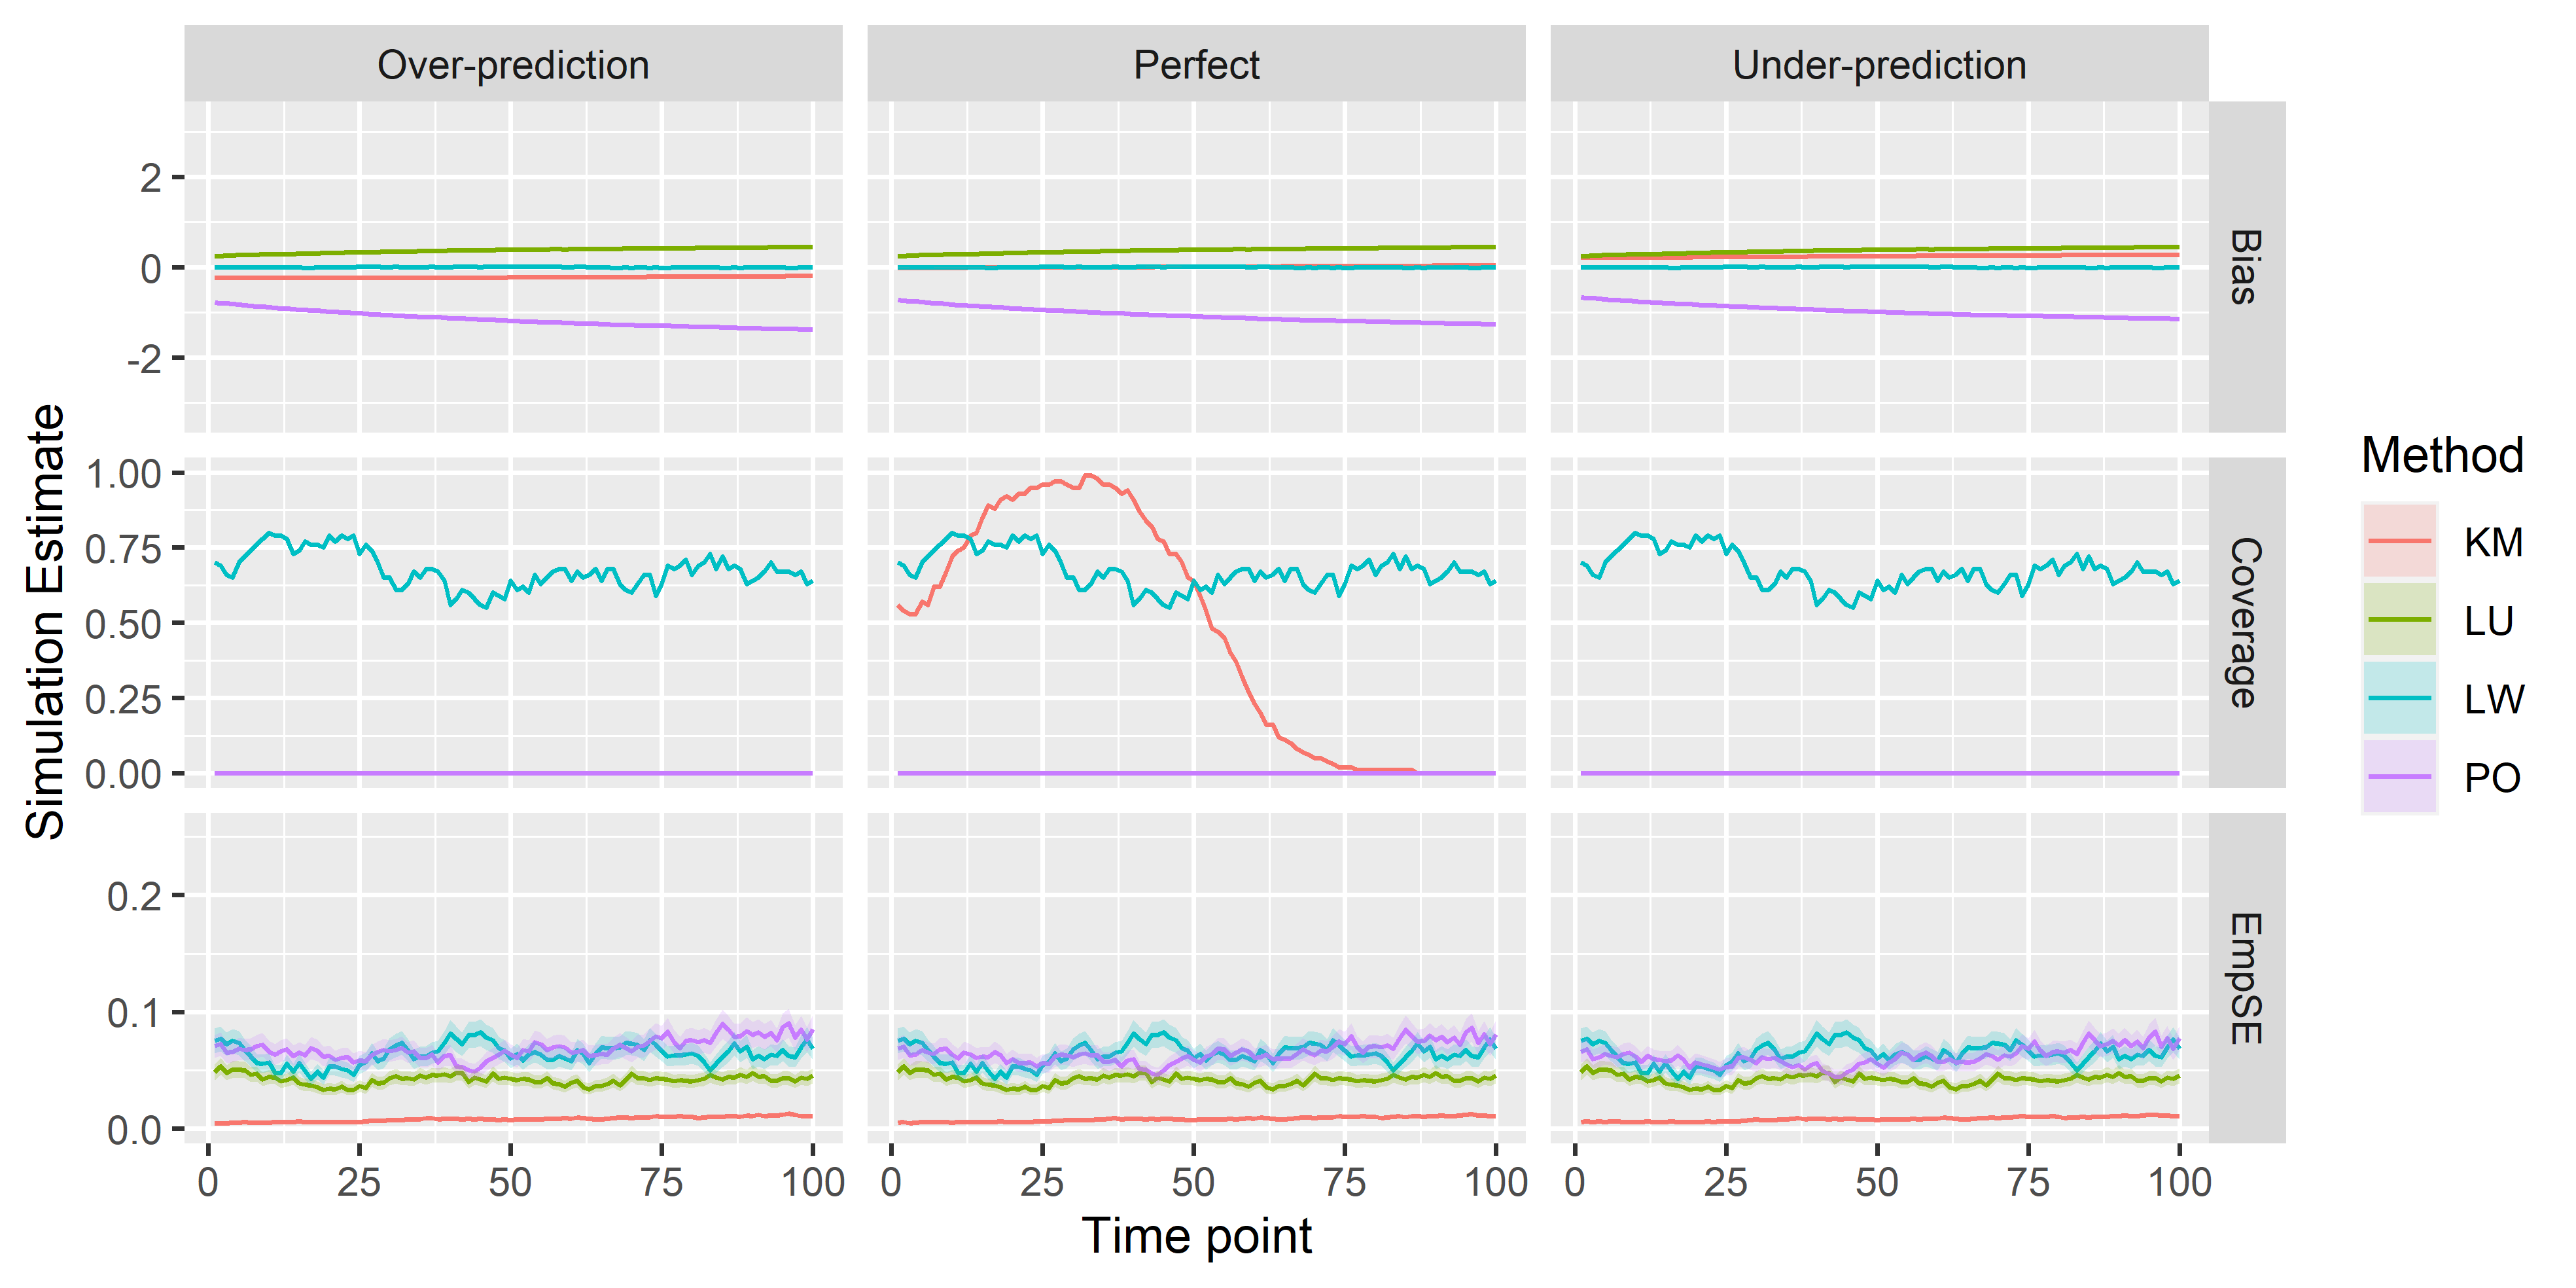
\includegraphics[width=54.68in]{figure/IPCW_Logistic/MainPlot_b(1)_g(1)_e(0.5)} \caption{Bias, Coverage and Empirical Standard Error for the Over-estimating, Perfect and Under-Estimating models across all four methods when $\beta=1$, $\gamma=1$ and $\eta=\sfrac{1}{2}$. Confidence Intervals are included in the plot, but are tight around the estimate}\label{fig:MainPlotg1}
\end{figure}
Figure \ref{fig:MainPlotg1} shows the results when censoring and the event-of-interest have the same individual effects (\(\beta=\gamma=1\)). The LW method provides strong coverage across the entire timeframe and miminal bias, although this coverage is reduced compared to the previous set of results shown (approximately 75\% throughout). Once again, the absolute bias for PO and LU increases over time, however the under-reporting for PO is much more strongly pronounced. KM bias behaves similarly but for coverage, it starts off at around 50\% coverage reaches a peak of full coverage approximately 25\% of the way through the timeframe.
\begin{figure}
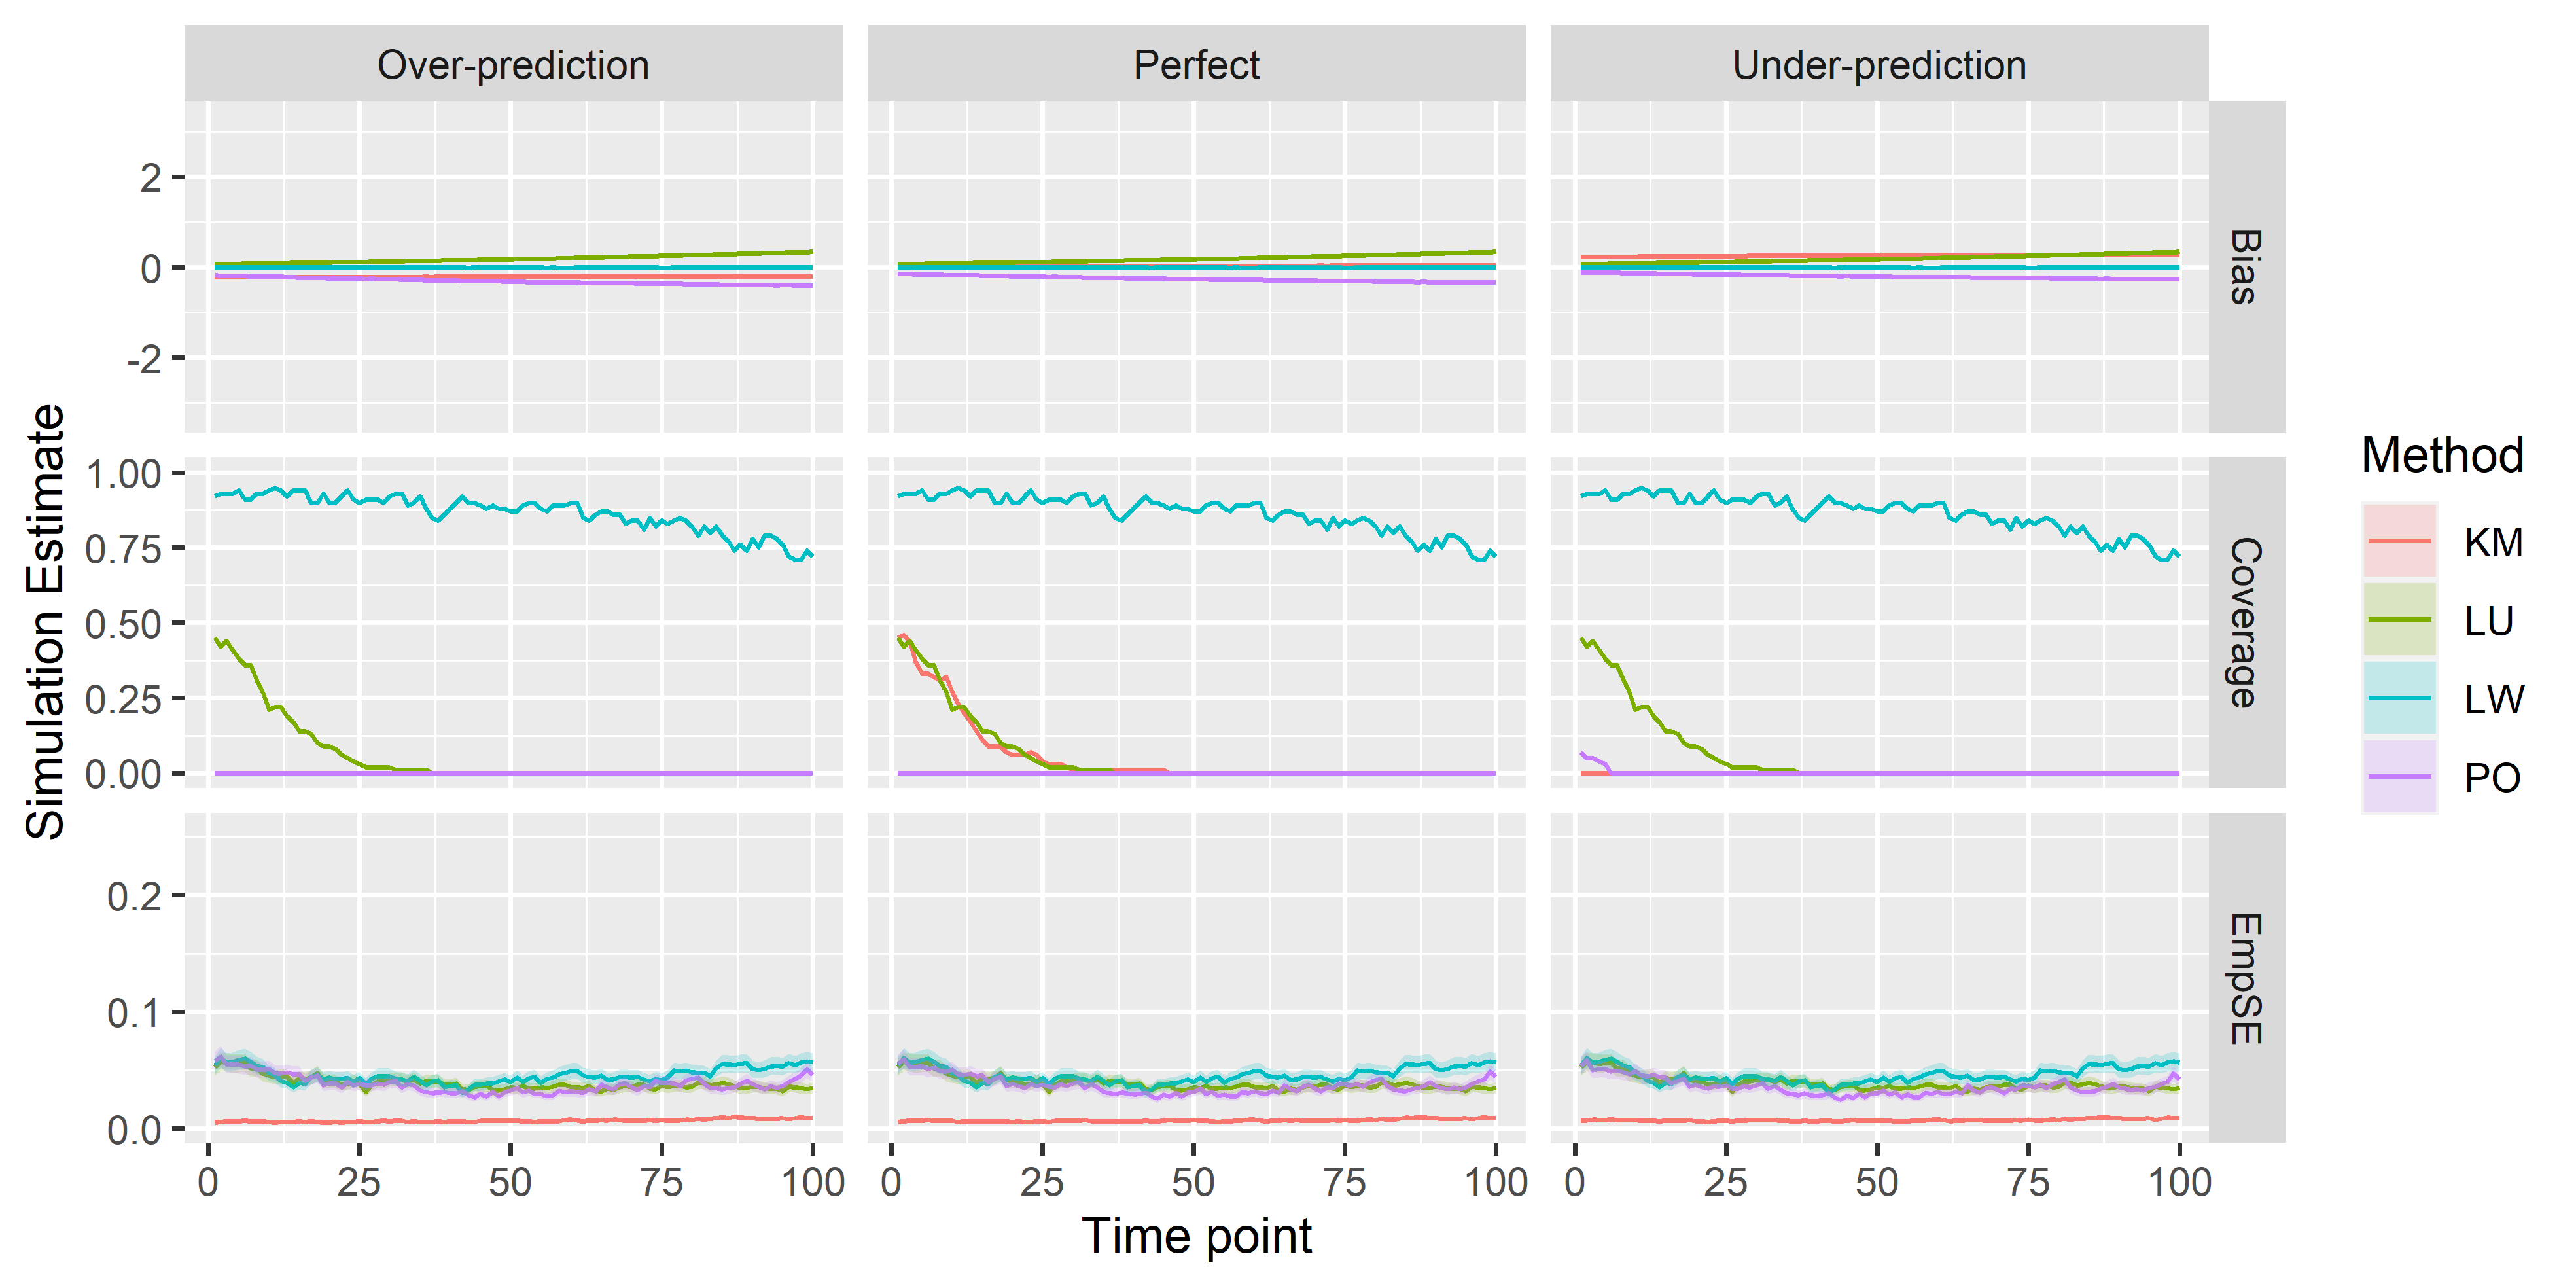
\includegraphics[width=54.68in]{figure/IPCW_Logistic/MainPlot_b(1)_g(-1)_e(0.5)} \caption{Bias, Coverage and Empirical Standard Error for the Over-estimating, Perfect and Under-Estimating models across all four methods when $\beta=1$, $\gamma=-1$ and $\eta=\sfrac{1}{2}$. Confidence Intervals are included in the plot, but are tight around the estimate}\label{fig:MainPlotg2}
\end{figure}
Figure \ref{fig:MainPlotg2} shows the results when censoring and the event-of-interest have opposite individual effects (\(\beta=1, \gamma=-1\)). The bias results are similar to those when censoring is independent. A difference here is that coverage begins greater than zero for the KM, LU and PO methods, but quickly drops to 0 before the 25\% time point. For LW, the coverage appears to reduce to around 80\% by the end of the time point.

\hypertarget{discussion-2}{%
\section{Discussion}\label{discussion-2}}

Weighting = Good.

Not Weighting = Bad.

\textbf{limitation}: Maybe the ``True'' \(\theta\) for the under and over predictions were wrong and that would explain the low Coverage.

\hypertarget{chap-performance-metrics}{%
\chapter{Prediction Model Performance Metrics for the Validation of Multi-State Clinical Prediction Models}\label{chap-performance-metrics}}

\emph{MA Barrowman, GP Martin, N Peek, M Lambie, M Sperrin}
\chaptermark{Development and Validation of MSCPM}
Last updated: 30 Apr

\hypertarget{introduction-5}{%
\section{Introduction}\label{introduction-5}}

Clinical Prediction Models (CPMs) provide individualised risk of a patient's outcome (cite), based on that patient's predictors. These predictions will usually be in the form of a risk score or probability. However, using traditional modelling techniques, these CPMs will only predict a single outcome. Multi-State Clinical Prediction Models (MS-CPMs) combine the multi-state modelling framework to the prognostic field to provide predictions for multiple outcomes in a single model.
Once a CPM has been developed, it is important to assess how well the model actually performs (cite). This process is called Model Validation and involves comparing the predictions produced by the model to the actual outcomes experienced by patients (cite). It is expected that the development of a CPM will be accompanied by the validation of the model on the same dataset it was developed in (internal validation), using either bootstrapping or cross-validation to account for optimism in the developed model (cite). Models can also be validated on a novel dataset (external validation), which is used to assess the generalisability and transportability of the model (cite).
During validation, there are different aspects of model performance that we can assess and these are measured using specific metrics. For example, to assess the overall Accuracy of a model, we may use the Brier Score (cite) or to analyse how well a model discriminates between patients, we could use the c-statistic (cite). The current metrics that are commonly used have been designed and extended to work in a variety of model development frameworks. However, these extensions are limited to either a single outcome (as in traditionally developed models) or do not adequately account for the censoring of patients (as commonly occurs in longitudinal data).
This paper aims to provide use-able extensions to current performance metrics to be used when validating MS-CPMs. It is essential that these extensions are directly comparable with current metrics (to allow for quicker adoption), that they are collapsible to the current metrics and that they adjust for the bias induced by the censoring of patients.
Currently, the most common way to validate an MS-CPMs is by applying traditional methods to compare across two states at a given time and then aggregating the results in an arbitrary manner {[}cite something{]}. Other methodologists have extended existing metrics to multinomial outcomes {[}cite van Calster{]}, which do not contain a time-based component; to simple competing risks scenarios {[}cite CR c-statistic{]}, which do not contain transient states; or to {[}\ldots{} insert third relevant example{]}. Spitoni et al {[}cite Spitoni 2018{]}{]} developed methods to apply the Brier Score (or any proper score functions) to a multi-state setting and so a simplified and specific version of their work is described in this paper.
It is the hope of the authors that this work will increase the uptake of multi-state models and the sub-field of MS-CPMs will grow appropriately.

\hypertarget{motivating-data-set}{%
\section{Motivating Data Set}\label{motivating-data-set}}

{[}\textbf{Table One for The Glasgow Data}{]}

Throughout this paper we will use a model developed in Chronic Kidney Disease (CKD) patients to assess their progression onto Renal Replacement Therapy (RRT) and/or Death {[}cite Dev/Valid Paper{]}. The model was developed using data from the Salford Kidney Study (SKS) and then applied to an external dataset derived from the West of Scotland (see Table 2) {[}1{]}. The original model predicts the probability that a patient has begun RRT and/or died after their first recorded eGFR below 60 ml/min/1.73m2, by any time in the future (reliable up to 10 years). For the purposes of this paper, we will take a ``snapshot'' of the predictions at the 5 year time point.
The Three-State model used in our example is designed as an Illness-Death Model {[}2{]}, this is one of the simplest MSM designs and has the key advantage over a traditional model that they can predict whether a patient is in or has visited the transient state before reaching the absorbing state (i.e.~patient who became ill before dying or who started RRT before dying) (see figure 1).

{[}\textbf{Figure of the MSM}{]}

{[}\textbf{Describe Glasgow Data}{]}

\hypertarget{current-approaches}{%
\section{Current Approaches}\label{current-approaches}}

Here we describe three commonly used performance metrics for assessing the performance of a traditional survival clinical prediction model. These metrics assess the Accuracy, Discrimination and Calibration of the models being validated. Accuracy is an overall measurement of how well the model predicts the outcomes in the patients. Discrimination assesses how well the model discerns between patients; in a two-state model this is a comparison of patients with and without the outcome, and should assign a higher value to those that experience the outcome. Calibration is the agreement between the observed outcomes and the predicted risks across the full risk-range.
We are applying cross-sectional metrics at a set time point within the setting of a longitudinal model and so we need to account for the censoring of patients and therefore, each uncensored patient at a given time t will be weighted as per the Inverse Probability of Censoring Weighting (IPCW) {[}3{]}. This allows the uncensored patient population to be representative of the entire patient population.

\hypertarget{baseline-models}{%
\subsection{Baseline Models}\label{baseline-models}}

To assess the performance of a model, we must compare the values produced by the performance metrics to those of two baseline models; a random or noninformative model and a perfect model.
A Non-Informative (NI-)model assigns the same probability to all patients to be in any state regardless of covariates and is akin to using the average prevalence in the entire population to define your model. For example, in a Two-State model and an event that occurs in 10\% of patients, all patients are predicted to have a 10\% chance of having the event. For many metrics, models can be compared to a Non-Informative model to assess whether the model is in fact ``better than random''.
A Perfect (P-)model is one which successfully assigns a 100\% probability to all patients, and the predictions are correct; this is the ideal case, which many models can also be compared to as models as close to this display excellent predictive abilities. Although models may perform worse than a non-informative one, we will not consider these in detail here as they are considered to be without worth in terms of predictive ability.
The metrics produced by these baseline models will often depend on the prevalence of each state and/or the number of states. These values can be used as comparators to provide contextual information regarding the strength of model performance. These baselines metrics for the NI-model and the P-model will be referred to as the NI-level and P-level for the metric.
In order to allow for simplicity and understanding of these measures, they will be standardised to the same scales.

\hypertarget{notation}{%
\subsection{Notation}\label{notation}}

Throughout this paper, we will use consistent notation which is shown here for reference and to avoid repetition in definitions, etc\ldots{}

{[}\textbf{Notation Table}{]}

\hypertarget{patient-weighting}{%
\subsection{Patient Weighting}\label{patient-weighting}}

{[}\textbf{Lots of formula, so will leave for now}{]}

\hypertarget{accuracy---brier-score}{%
\subsection{Accuracy - Brier Score}\label{accuracy---brier-score}}

\hypertarget{discrimination---c-statistic}{%
\subsection{Discrimination - c-statistic}\label{discrimination---c-statistic}}

\hypertarget{calibration---intercept-and-slope}{%
\subsection{Calibration - Intercept and Slope}\label{calibration---intercept-and-slope}}

\hypertarget{extension-to-multi-state-models}{%
\section{Extension to Multi-State Models}\label{extension-to-multi-state-models}}

\hypertarget{trivial-extensions}{%
\subsection{Trivial Extensions}\label{trivial-extensions}}

\hypertarget{accuracy---multiple-outcome-brier-score}{%
\subsection{Accuracy - Multiple Outcome Brier Score}\label{accuracy---multiple-outcome-brier-score}}

\hypertarget{discrimination---polytomous-discriminatory-index}{%
\subsection{Discrimination - Polytomous Discriminatory Index}\label{discrimination---polytomous-discriminatory-index}}

\hypertarget{computational-limitations}{%
\subsubsection{Computational Limitations}\label{computational-limitations}}

\hypertarget{calibration---multinomial-intercept-matched-and-unmatched-slopes}{%
\subsection{Calibration - Multinomial Intercept, Matched and Unmatched Slopes}\label{calibration---multinomial-intercept-matched-and-unmatched-slopes}}

\hypertarget{application-to-real-world-data}{%
\section{Application to Real-World Data}\label{application-to-real-world-data}}

\hypertarget{accuracy}{%
\subsection{Accuracy}\label{accuracy}}

\hypertarget{discrimination}{%
\subsection{Discrimination}\label{discrimination}}

\hypertarget{calibration}{%
\subsection{Calibration}\label{calibration}}

\hypertarget{discussion-3}{%
\section{Discussion}\label{discussion-3}}

\hypertarget{chap-dev-paper}{%
\chapter{Development and External Validation of a Multi-State Clinical Prediction Model for Chronic Kidney Disease Patients Progressing onto Renal Replacement Therapy and Death}\label{chap-dev-paper}}

\emph{MA Barrowman, GP Martin, N Peek, M Lambie, W Hulme, R Chinnadurai, J Lees, P Kalra, P Mark, J Traynor, M Sperrin}
\chaptermark{Development and Validation of MSCPM}
Last updated: 29 Apr

\hypertarget{abstract-2}{%
\section*{Abstract}\label{abstract-2}}
\addcontentsline{toc}{section}{Abstract}

\hypertarget{introduction-6}{%
\subsection*{Introduction}\label{introduction-6}}
\addcontentsline{toc}{subsection}{Introduction}

Clinical Prediction Models (CPMs) provide individualised predictions for patient outcomes. Traditionally, these models provide predictions for single outcomes, however in many circumstances, the ability to predict multiple outcomes with a single model can be advantageous. Multi-State Models are a method to provide these kinds of predictions.

\hypertarget{methods-5}{%
\subsection*{Methods}\label{methods-5}}
\addcontentsline{toc}{subsection}{Methods}

We developed a Multi-State Clinical Prediction Model (MSCPM) using tertiary care data from the Salford Kidney Study as our development data set and secondary care data from the West of Scotland (SERPR) dataset as our validation set. We developed three models of different levels of complexity; a Two-State Model (Alive and Dead), a Three-State Model (Untreated CKD, Renal Replacement Therapy and Dead) and a Five-State model (Untreated CKD, Haemodialysis, Peritoneal Dialysis, Transplant and Dead). We used Royston-Parmer regression techniques to allow us to provide individualised predictions for patients. Model performance was assessed for accuracy, discrimination and calibration using methods both internally and externally. The best performing model was used to produce a CPM Calculator for clinical use.

\hypertarget{results-4}{%
\subsection*{Results}\label{results-4}}
\addcontentsline{toc}{subsection}{Results}

Of the three models produced, Age was a strong predictor of mortality in all cases and outcomes were highly dependent on primary renal diagnosis. Models performed well in both the internal and external validation with the Three-State Model out performing overall. The Three-State Model was used to develop the online Calculator.

\hypertarget{discusssion}{%
\subsection*{Discusssion}\label{discusssion}}
\addcontentsline{toc}{subsection}{Discusssion}

Our CPMs provide clinicians and patients with multiple outcome predictions. This implies that users of these models can get more information about their potential future without a loss to the quality of that prediction.

\hypertarget{supplementary-material-2}{%
\subsection*{Supplementary Material}\label{supplementary-material-2}}
\addcontentsline{toc}{subsection}{Supplementary Material}

Supplementary Material is available in Appendix \ref{chap-dev-paper-supp}.

\hypertarget{introduction-7}{%
\section{Introduction}\label{introduction-7}}

A clinical prediction model (CPM) is a tool which provides patients and clinicians with a measure of how likely a patient is to suffer a specific clinical condition, more specifically, a prognostic model allows the prediction of future events {[}\protect\hyperlink{ref-steyerberg_prognosis_2013}{8}{]}. CPMs use data from previous patients to estimate the outcomes of an individual patient. Prognostic models are used in clinical practice to influence treatment decisions such as the prescribing of statins for cardiovascular disease via the application of the QRISK models {[}\protect\hyperlink{ref-hippisley-cox_development_2017}{2}{]}.

Within Chronic Kidney Disease (CKD), prognostic models have been developed to predict mortality {[}\protect\hyperlink{ref-johnson_predicting_2007}{56}{]}--{[}\protect\hyperlink{ref-wick_clinical_2017}{60}{]}, ESRD {[}\protect\hyperlink{ref-landray_prediction_2010}{57}{]}, the commencements of RRT {[}\protect\hyperlink{ref-marks_looking_2015}{59}{]}, {[}\protect\hyperlink{ref-johnson_predicting_2008}{61}{]}--{[}\protect\hyperlink{ref-kulkarni_transition_2017}{63}{]} or mortality after beginning dialysis {[}\protect\hyperlink{ref-floege_development_2015}{64}{]}--{[}\protect\hyperlink{ref-cao_predicting_2015}{66}{]}. Some previous models have used the commencement of RRT as a proxy for ESRD {[}\protect\hyperlink{ref-tangri_predictive_2011}{67}{]}--{[}\protect\hyperlink{ref-tangri_dynamic_2017}{69}{]}, while others have investigated the occurrence of cardiovascular events within CKD patients{[}\protect\hyperlink{ref-shlipak_cardiovascular_2005}{70}{]}--{[}\protect\hyperlink{ref-mcmurray_predictors_2011}{72}{]}. Reviews by Grams \& Coresh {[}\protect\hyperlink{ref-grams_assessing_2013}{73}{]}, Tangri et al {[}\protect\hyperlink{ref-tangri_risk_2013}{74}{]} and Ramspek et al {[}\protect\hyperlink{ref-ramspek_prediction_2017}{75}{]}, which explored the different aspects of assessing risk amongst CKD or RRT patients, found that the current landscape of CKD prediction models is lacking from both a methodological and clinical perspective {[}\protect\hyperlink{ref-collins_transparent_2015}{13}{]}, {[}\protect\hyperlink{ref-bouwmeester_reporting_2012-1}{76}{]}.

Methodologically, the majority of existing CKD prediction models fail to account for completing events {[}\protect\hyperlink{ref-bansal_development_2015}{58}{]}, {[}\protect\hyperlink{ref-wick_clinical_2017}{60}{]}, {[}\protect\hyperlink{ref-perotte_risk_2015}{77}{]}, have high risks of bias {[}\protect\hyperlink{ref-johnson_predicting_2007}{56}{]}, {[}\protect\hyperlink{ref-landray_prediction_2010}{57}{]}, {[}\protect\hyperlink{ref-johnson_predicting_2008}{61}{]} or are otherwise flawed compared to modern clinical prediction standards {[}\protect\hyperlink{ref-steyerberg_prognosis_2013}{8}{]}, {[}\protect\hyperlink{ref-collins_transparent_2015}{13}{]}

In 2013, Begun et al {[}\protect\hyperlink{ref-begun_identification_2013}{78}{]} developed a multi-State model for assessing population-level progression through the severity stages of CKD (III-V), RRT and/or death, which can be used to provide a broad statement regarding a patient's future. In 2014, Allen et al {[}\protect\hyperlink{ref-allen_chronic_2014}{79}{]} applied a similar model to liver transplant recipients and their progression through the stages of CKD with a focus on the predictions of measured vs estimated glomerular filtration rate (mGFR vs eGFR). In 2017, Kulkarni et al {[}\protect\hyperlink{ref-kulkarni_transition_2017}{63}{]} developed an MSM focusing on the categories of Calculated Panel Reactive Antibodies (CPRA) and kidney transplant and/or death.

Most recently, in 2018, Grams et al {[}\protect\hyperlink{ref-grams_predicting_2018}{80}{]} developed a multinomial clinical prediction model for CKD patients which focused on the occurrence of RRT and/or cardiovascular events. As of the publication of this paper, this is the only currently existing CPMs of this kind for CKD patients.

However, the first three of these existing models (Begun, Allen and Kulkarni) categorise continuous variables to define their states at specific cut-offs and this has been shown to be inefficient when modelling {[}\protect\hyperlink{ref-royston_dichotomizing_2006}{17}{]}, {[}\protect\hyperlink{ref-altman_problems_1994-1}{81}{]}--{[}\protect\hyperlink{ref-weinberg_how_1995}{98}{]}. These kinds of cut-offs can be useful when informing patients and clinicians of a patient's diagnosis and to coincide with policy, but inherently cause a loss of information when done before the data analysis stage and so these models go against current statistical recommendations {[}\protect\hyperlink{ref-royston_dichotomizing_2006}{17}{]}, {[}\protect\hyperlink{ref-altman_problems_1994-1}{81}{]}--{[}\protect\hyperlink{ref-weinberg_how_1995}{98}{]}. These kinds of assumptions are also subject to measurement error {[}\protect\hyperlink{ref-van_smeden_reflection_2019}{99}{]} and interval censoring {[}\protect\hyperlink{ref-sun_interval_2005}{100}{]}, i.e.~we do not know when exactly when a patient moved from CKD Stage III to CKD Stage IV, or whether drop in estimated Glomerular Function Rate (eGFR) was temporary or inaccurate. For example, Kulkarni {[}\protect\hyperlink{ref-kulkarni_transition_2017}{63}{]} assumes that a patient with an CPRA of (5\%) is the same as a patient with an CPRA of (75\%) and that a patient with an CPRA of (89.9\%) is vastly different from a patient with an CPRA of (90\%). Moreover, none of these models have undergone any validation process, whether internal or external {[}\protect\hyperlink{ref-altman_prognosis_2009}{10}{]}.

It is also important to note that although these models can be used to predict patient outcomes, they were not designed to produce individualised patient predictions as is a key aspect of a clinical prediction model; they were designed to assess the methodological advantages of MSMs in this medical field, to describe the prevalence of over time of different CKD stages and to produce population level predictions for patients with different levels of panel-reactive antibodies {[}\protect\hyperlink{ref-royston_prognosis_2009}{9}{]}.

The fourth model (Grams), is presented as a Multi-State Model and the transitions involved were studied and defined, however the underlying statistical model is a pair of multinomial logistic models analysed at 2 and 4 years. The major downside of this model is that it can only produce predictions at those predefined time points and it assumes homogeneity of transition times. For example, the first model assumes that a patient who began RRT 1 month after study entry is the same as one who began after 1 year \& 11 months into the study and then the second model assumes these patients are the same as one who begins RRT at 3 years and 11 months.

Therefore, the aim of this study was to improve on previous efforts to model a patient's pathways through a Multi-State Model by choosing transition points which can be exactly identified and include states which produce a drastic difference in patient characteristics. Our modeling techniques allow for individual predictions (using a proportional hazards model) of multiple outcomes (using MSMs) at any time point (using cubic splines). The models produced by this process will then be validated, both internally and externally, to compare their results and demonstrate the transportability of the (statistically robust) clinical prediction models. We report our work in line with the TRIPOD guidelines for development and validation of clinical prediction models {[}\protect\hyperlink{ref-collins_transparent_2015}{13}{]}, {[}\protect\hyperlink{ref-moons_transparent_2015}{14}{]}.

\hypertarget{methods-6}{%
\section{Methods}\label{methods-6}}

\hypertarget{data-sources}{%
\subsection{Data Sources}\label{data-sources}}

The models were developed using data from the Salford Kidney Study (SKS) cohort of patients (previously named the CRISIS cohort), established in the Department of Renal Medicine, Salford Royal NHS Foundation Trust (SRFT). The SKS is a large longitudinal CKD cohort recruiting CKD patients since 2002. This cohort collects detailed annualised phenotypic and laboratory data, and plasma, serum and whole blood stored at -80\textdegree C for biomarker and genotypic analyses. Recruitment of patients into SKS has been described in multiple previous studies {[}\protect\hyperlink{ref-hoefield_factors_2010}{101}{]}, {[}\protect\hyperlink{ref-chinnadurai_increased_2019-1}{102}{]} and these have included a CKD progression prognostic factor study and to evidence the increased risk of cardiovascular events in diabetic kidney patients. In brief, any patient referred to Salford renal service (catchment population 1.5 million) who is 18 years or over and has an eGFR measurement of less than \(60\textrm{ml}/\textrm{min}/1.73\textrm{m}^2\) (calculated using the CKD-EPI formula {[}\protect\hyperlink{ref-levey_new_2009}{103}{]}) was approached to be consented for the study participation.

At baseline, the data, including demographics, comorbidities, physical parameters, lab results and primary renal diagnosis are recorded in the database. Patients undergo an annual study visit and any changes to these parameters are captured. All data except blood results are collected via questionnaire by a dedicated team of research nurses. Blood results (baseline and annualised), first RRT modality and mortality outcome data are directly transferred to the database from Salford's Integrated Record (SIR) {[}\protect\hyperlink{ref-new_obtaining_2014}{104}{]}. eGFR, uPCR, comorbidity and blood results were measured longitudinally throughout a patient's time within the cohort.

Due to limitations in our data, we were agnostic to how long since patients were diagnosed with CKD. Therefore, we defined a patient's start date for our model as their first date after consent at which their eGFR was recorded to be below \(60\textrm{ml}/\textrm{min}/1.73\textrm{m}^2\). Some patients consented with an eGFR that was already below 60, and some entered our study later when their eGFR was measured to be below 60. This implies that our models includes both patient who have recently been diagnosed with CKD (\(\textrm{eGFR} \lessapprox 60\)) \emph{and} those that have been suffering with CKD for an arbitrary amount of time. This timelessness of the model means it can be applied to any patient at any time during their CKD journey.

This allows for a wider range of baseline eGFR measurements and patients who have been suffering from CKD, translating to a model which can be applied to

All patients registered in the database between October 2002 and December 2016 with available data were included in this study. As this is a retrospective convenience sample, no sample size calculations were performed prior to recruitment. All patients were followed-up within SKS until the end-points of RRT, death or loss to follow-up or were censored at their last interaction with the healthcare system prior to December 2017. Date of death for patients who commenced RRT was also available within SIR and so also included in the SKS database.

For external validation of the model, we extracted an independent cohort from the West of Scotland Electronic Renal Patient Record (SERPR). Our extract of SERPR contains all patients known to the Glasgow and Forth Valley renal service who had an eGFR measure of less than \(60\textrm{ml}/\textrm{min}/1.73m^2\) between January 2006 and January 2016. This cohort has been previously used in Chronic Kidney Disease Prognosis consortium studies investigating outcomes in patients with CKD {[}\protect\hyperlink{ref-matsushita_cohort_2013}{105}{]} and a similar cohort has been used for the analysis of skin tumours amongst renal transplant patients. Use of anonymised data from this database has been approved by the West of Scotland Ethics Committee for use of NHS Greater Glasgow and Clyde `Safe Haven' data for research.

Both the internal and external validation cohort were used as part of the multinational validation cohort used by Grams et al in their multinomial CPM discussed above {[}\protect\hyperlink{ref-grams_predicting_2018}{80}{]}. In SERPR, start dates were calculated to be the first time point where the following conditions were met:
\begin{itemize}
\tightlist
\item
  eGFR is measured at less than 60
\item
  There is at least one prior eGFR measurement
\item
  Patient is 18 or over
\item
  Patient is not enduring an AKI {[}\protect\hyperlink{ref-forni_renal_2017-1}{106}{]}, {[}\protect\hyperlink{ref-noauthor_kdigo_2012}{107}{]}.
\end{itemize}
The second requirement was implemented to avoid a bias in the eGFR Rate. eGFR Rate is a measure of the change in eGFR over time and is calculated as the difference between the most recent two eGFR measurements divided by the time between them. For patients who entered the system with an \(\textrm{eGFR} < 60\), their eGFR Rate would be unavailable (i.e.~missing). Otherwise, patient eGFRs would \emph{have} to drop to below 60 and thus eGFR Rate would be negative.

\hypertarget{model-design}{%
\subsection{Model Design}\label{model-design}}

Three separate models were developed, so we could determine a clinically viable model while maintaining model parsimony as much as possible: a Two-State, Three-State and Five-State model, each building on the previous models' complexity (see figure \ref{fig:State-Diagram}). The Two-State model was a traditional survival analysis where a single event (death) is considered. The Three-State model expanded on this, by splitting the Alive state into transient states of (untreated) CKD and (first) RRT; patients can therefore transition from CKD to Death or CKD to RRT, and then onto RRT to Death. The Five-State model stratifies the RRT state into HD, PD and Tx and allows similar transitions into and out of the RRT states; however, the transition from Tx to Death was not considered as it was anticipated a priori that there would be insufficient patients undergoing this transition and that the process of undergoing a transplant would be medically transformative and so it would be inappropriate to assume shared parameters before and after the transition (i.e.~Tx was modelled as a second absorbing state).
\begin{figure}

{\centering 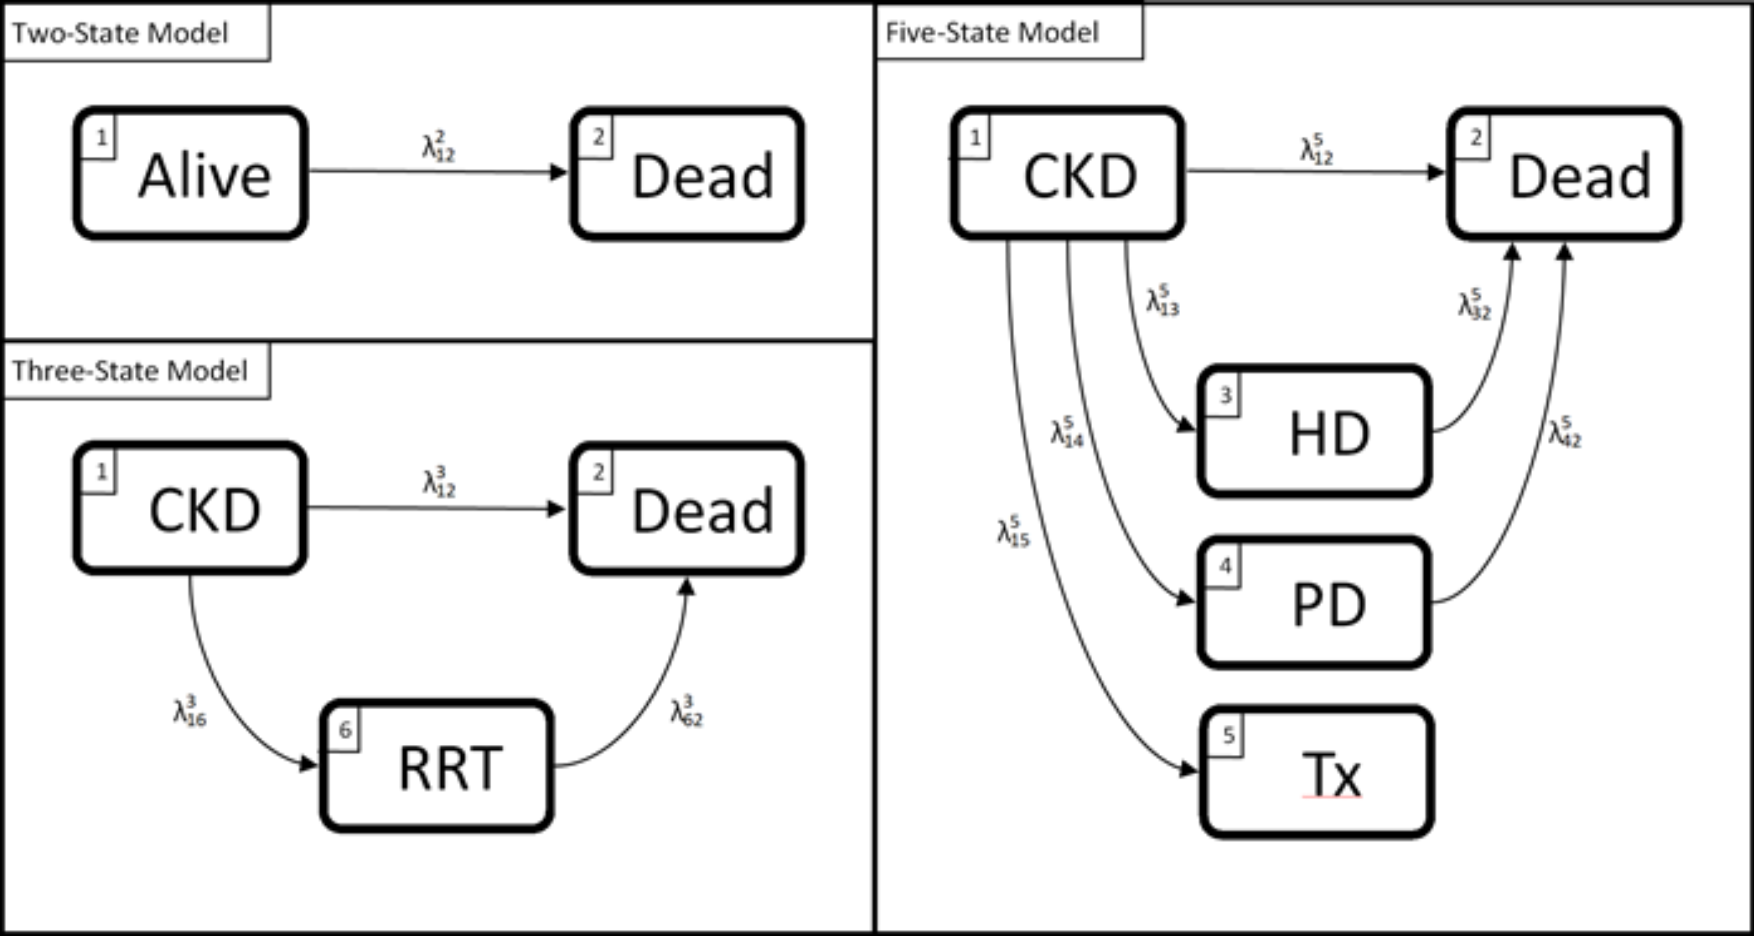
\includegraphics[width=0.9\linewidth]{figure/Dev_Paper_State_Diagrams} 

}

\caption{Diagram of the three models, the states being modelled and relevant transitions}\label{fig:State-Diagram}
\end{figure}
The models were developed and validated as discussed in the Supplementary materials in appendix \ref{chap-dev-paper-supp}.

\hypertarget{example}{%
\subsection{Example}\label{example}}

Once the models have been developed, we will apply them to two example patients to demonstrate their use and applicability to the general population. We will provide a direct clinical estimation of these patient outcomes based on years of nephrological experience and compare this with the results presented by our clinical prediction model.

We have chosen three (synthetic) patients to use as examples of the use of our model. Their details can be seen in table \ref{tab:Example-Patient}.
\begin{table}[!h]

\caption{\label{tab:Example-Patient}{\small Details of the Example Patients}}
\centering
\fontsize{7}{9}\selectfont
\begin{tabular}[t]{>{\raggedright\arraybackslash}p{3.5cm}>{\raggedright\arraybackslash}p{3.5cm}>{\raggedright\arraybackslash}p{3.5cm}>{\raggedright\arraybackslash}p{3.5cm}}
\toprule
  & Patient 1 & Patient 2 & Patient 3\\
\midrule
\rowcolor{gray!6}  Age & 20 & 40 & 66\\
Gender & Female & Male & Female\\
\rowcolor{gray!6}  Smoking Status & Non-Smoker & Smoker & Non-Smoker\\
BP & 144/101 & 160/90 & 140/80\\
\rowcolor{gray!6}  Albumin & 39 & 40 & 40\\
\addlinespace
Correct Calcium & 2.3 & 3.0 & 2.6\\
\rowcolor{gray!6}  Haemoglobin & 150 & 100 & 14\\
Phosphate & 0.68 & 2.00 & 0.86\\
\rowcolor{gray!6}  eGFR & 42 & 10 & 51\\
eGFR Previous & 50 (one week ago) & 30 (one year ago) & 70 (one week ago)\\
\addlinespace
\rowcolor{gray!6}  uPCR & 0.30 & 0.20 & 0.01\\
uPCR Previous & 0.80 (one month ago) & 1.20 (one year ago) & 0.06 (one week ago)\\
\rowcolor{gray!6}  Primary Diagnosis & Glomerulonephritis & Tubular Necrosis & Diabetes\\
Comorbities & Chronic Obstructive Pulmonary Disease\newline Liver Disease\newline Solid Tumour &  & Diabetes\newline Chronic Obstructive Pulmonary Disease\newline Hypertension\\
\bottomrule
\end{tabular}
\end{table}
Out three example patients cover a broad range of ages and other covariates. A clinically guided prediction for these patients would assume that Patient 1 has a high chance of proceeding as normal (with little need for RRT), Patient 2 would be recommended to start RRT soon and Patient 3 would be predicted to have a high risk of mortality with or without RRT.

\hypertarget{calculator}{%
\subsection{Calculator}\label{calculator}}

As part of this work, we also intend to produce an online calculator to allow patients and clinicians to easily estimate outcomes without worrying about the mathematics involved.

All analysis was done in \texttt{R\ 3.6.2} {[}\protect\hyperlink{ref-r_core_team_r_nodate}{51}{]} using the various \texttt{tidyverse} packages {[}\protect\hyperlink{ref-wickham_tidy_2017}{52}{]}, as well as the \texttt{mice} {[}\protect\hyperlink{ref-buuren_mice_2011-1}{108}{]}, \texttt{flexsurv} {[}\protect\hyperlink{ref-jackson_flexsurv_nodate}{109}{]}, \texttt{nnet} {[}\protect\hyperlink{ref-ripley_package_2016}{110}{]} and \texttt{furrr} {[}\protect\hyperlink{ref-vaughan_furrr_2018}{111}{]} packages. The calculator was produced using the \texttt{shiny} package {[}\protect\hyperlink{ref-chang_shiny_2020}{55}{]}.

\hypertarget{results-5}{%
\section{Results}\label{results-5}}

\hypertarget{data-sources-1}{%
\subsection{Data Sources}\label{data-sources-1}}

As seen in table \ref{tab:Continuous-Demo}, The Age of both populations were centred around 64-65 with a very broad range. Due to the inclusion criteria, eGFR were capped at a maximum of 60, and was consistent across populations; however, the rate of change for eGFR was much wider in the SERPR patients than in the SKS, and it was decreasing much faster, on average ( -25 vs 0) . Blood pressure was also consistent across populations (140/75 vs 148/76 for development vs validation). The blood test results (Corrected Calcium, Albumin, Haemoglobin and Phosphate) was close together, with the further difference being Haemoglobin with an average of 123 in SKS and 109 in SERPR and a much larger standard deviation in SERPR compared to SKS (38 vs 17). The uPCR measures are presented in our results as g/mmol, rather than the more conventional g/mol, this is to better present results and coefficients of varying magnitudes. Similar to the eGFR measures, the uPCR results were similar, but the rates of change were much broader in the validation dataset compared to the SKS and were generally increasing, whereas SKS remained stationary (73 vs 0). Levels of missingness were much higher in the SERPR dataset in most continuous variables.

\newgeometry{margin=2cm}
\begin{landscape}\begin{table}

\caption{\label{tab:Continuous-Demo}{\small Population demographics for the continuous variables presented as: mean (IQR) [min,max] <number missing (percent missing)>}}
\centering
\fontsize{7}{9}\selectfont
\begin{tabular}[t]{>{\raggedright\arraybackslash}p{13em}>{\ttfamily\raggedleft\arraybackslash}p{33em}>{\ttfamily\raggedleft\arraybackslash}p{36em}}
\toprule
  & SKS (Development) & SERPR (Validation)\\
\midrule
\rowcolor{gray!6}  \addlinespace[0.3em]
\multicolumn{3}{l}{\textbf{Age}}\\
\hspace{1em}Age & 64.378 (19.000) [ 20.000,  94.000] <    0 ( 0.00\%)> & 65.880 (17.000) [    18.000,    98.000] <    0 ( 0.00\%)>\\
\addlinespace[0.3em]
\multicolumn{3}{l}{\textbf{eGFR}}\\
\hspace{1em}eGFR\textsuperscript{a} & 30.368 (22.386) [  3.577,  59.965] <    0 ( 0.00\%)> & 36.132 (21.444) [     1.651,    59.998] <    0 ( 0.00\%)>\\
\rowcolor{gray!6}  \hspace{1em}eGFR Rate\textsuperscript{a} & -0.015 ( 0.293) [-19.107,  33.781] <1,278 (42.87\%)> & -25.476 (44.229) [-8,755.272, 9,260.375] <    0 ( 0.00\%)>\\
\addlinespace[0.3em]
\multicolumn{3}{l}{\textbf{uPCR}}\\
\hspace{1em}uPCR\textsuperscript{f} & 0.112 ( 0.103) [  0.000,   2.025] <  245 ( 8.21\%)> & 0.184 ( 0.147) [     0.000,     6.390] <7,513 (96.76\%)>\\
\rowcolor{gray!6}  \hspace{1em}uPCR Rate\textsuperscript{f} & -0.096 ( 0.188) [-70.727,  28.198] <1,777 (59.61\%)> & 73.177 ( 0.384) [    -2.255, 3,051.403] <7,721 (99.44\%)>\\
\addlinespace[0.3em]
\multicolumn{3}{l}{\textbf{Measures}}\\
\hspace{1em}SBP\textsuperscript{b} & 140.193 (29.000) [ 77.000, 220.000] <   50 ( 1.67\%)> & 147.746 (33.000) [    82.000,   258.000] <6,880 (88.61\%)>\\
\rowcolor{gray!6}  \hspace{1em}DBP\textsuperscript{b} & 74.555 (14.000) [ 36.000, 159.000] <   52 ( 1.74\%)> & 76.263 (18.000) [    35.000,   128.000] <6,879 (88.60\%)>\\
\hspace{1em}BMI\textsuperscript{c} & 28.848 ( 7.842) [ 13.182,  61.466] <  572 (19.18\%)> & 29.331 ( 7.851) [    15.343,    48.301] <7,681 (98.93\%)>\\
\rowcolor{gray!6}  \hspace{1em}Albumin\textsuperscript{d} & 42.152 ( 5.000) [ 12.000,  52.000] <   60 ( 2.01\%)> & 36.490 ( 6.000) [     7.000,    53.000] <3,455 (44.50\%)>\\
\hspace{1em}Corrected Calcium\textsuperscript{e} & 2.302 ( 0.180) [  1.209,   3.660] <   68 ( 2.28\%)> & 2.408 ( 0.160) [     1.419,     3.610] <5,113 (65.85\%)>\\
\rowcolor{gray!6}  \hspace{1em}Haemoglobin\textsuperscript{d} & 122.977 (23.000) [ 61.000, 195.000] <   72 ( 2.41\%)> & 108.588 (30.000) [     6.250,   208.000] <3,968 (51.10\%)>\\
\hspace{1em}Phosphate\textsuperscript{e} & 1.162 ( 0.320) [  0.430,   3.710] <   87 ( 2.91\%)> & 1.203 ( 0.320) [     0.370,     4.370] <5,127 (66.03\%)>\\
\bottomrule
\multicolumn{3}{l}{\textsuperscript{a} (ml/min/1.73m\textasciicircum{}2) or per year \textsuperscript{b} (mmHG) \textsuperscript{c} (kg/m\textasciicircum{}2) \textsuperscript{d} (g/l) \textsuperscript{e} (mmol/l) \textsuperscript{f} (g/mmol) or per year}\\
\end{tabular}
\end{table}
\end{landscape}
\restoregeometry

Table \ref{tab:Categorical-Demo} shows a breakdown of the categorical variables across the populations. In the development population, there are far more males than females, whereas in the validation population the proportions are much more matched. Most patients were white in the SKS dataset, and ethnicity has extremely high missingness in SERPR, which also contributed to its omission from the model. The majority of the SKS patients were former smokers, however this information was unavailable in the SERPR dataset. Primary Renal Diagnosis suffered from very high levels of missingness in the validation dataset, but was much better recorded in the development dataset (although still far from perfect).
\begin{table}[!h]

\caption{\label{tab:Categorical-Demo}{\small Population demographics for the categorical variables presented as number (percent)}}
\centering
\fontsize{7}{9}\selectfont
\begin{tabular}[t]{>{}l>{\ttfamily}r>{\ttfamily}r}
\toprule
  & SKS (Development) & SERPR (Validation)\\
\midrule
\rowcolor{gray!6}  \addlinespace[0.3em]
\multicolumn{3}{l}{\textbf{Gender}}\\
\hspace{1em}Male & 1,865 (62.56 \%) & 3,915 (50.42 \%)\\
\hspace{1em}Female & 1,116 (37.43 \%) & 3,849 (49.57 \%)\\
\rowcolor{gray!6}  \addlinespace[0.3em]
\multicolumn{3}{l}{\textbf{Ethnicity}}\\
\hspace{1em}White & 2,875 (96.44 \%) & 683 ( 8.79 \%)\\
\hspace{1em}Asian & 75 ( 2.51 \%) & 12 ( 0.15 \%)\\
\rowcolor{gray!6}  \hspace{1em}Black & 21 ( 0.70 \%) & 7 ( 0.09 \%)\\
\hspace{1em}Other & 10 ( 0.33 \%) & 2 ( 0.02 \%)\\
\rowcolor{gray!6}  \hspace{1em}<Ethnicity Missing> & 0 ( 0.00 \%) & 7,060 (90.93 \%)\\
\addlinespace[0.3em]
\multicolumn{3}{l}{\textbf{Smoking Status}}\\
\hspace{1em}Former & 1,535 (51.49 \%) & \\
\rowcolor{gray!6}  \hspace{1em}Non-Smoker & 979 (32.84 \%) & \\
\hspace{1em}Smoker & 379 (12.71 \%) & \\
\rowcolor{gray!6}  \hspace{1em}Former 3Y & 46 ( 1.54 \%) & \\
\hspace{1em}<Smoking Status Missing> & 42 ( 1.40 \%) & \\
\rowcolor{gray!6}  \addlinespace[0.3em]
\multicolumn{3}{l}{\textbf{Primary Renal Diagnosis}}\\
\hspace{1em}Systemic diseases affecting the kidney & 1,304 (43.74 \%) & 299 ( 3.85 \%)\\
\hspace{1em}Glomerular disease & 442 (14.82 \%) & 225 ( 2.89 \%)\\
\rowcolor{gray!6}  \hspace{1em}Tubulointerstitial disease & 268 ( 8.99 \%) & 164 ( 2.11 \%)\\
\hspace{1em}Miscellaneous renal disorders & 227 ( 7.61 \%) & 188 ( 2.42 \%)\\
\rowcolor{gray!6}  \hspace{1em}Familial / hereditary nephropathies & 173 ( 5.80 \%) & 102 ( 1.31 \%)\\
\hspace{1em}<Renal Diagnosis Missing> & 567 (19.02 \%) & 6,786 (87.40 \%)\\
\bottomrule
\end{tabular}
\end{table}
Overall, there were high levels of comorbidities within the SKS population as shown in table \ref{tab:Comorbidity-Demo}, but these levels were much lower in the SERPR population, possibly due to the data extraction processed (where data is un-recorded, no history is assumed). In SKS, most comorbidities were at over 80\% prevalence, apart from diabetes mellitus, which had a lower prevalence of 33\% and over 97\% (2,891) patients had a history of liver disease. In SERPR, hypertension was the highest prevalence in SERPR at 40\% (3,122), followed by diabetes mellitus at 20\% (1,546) and cerebrovascular accident was the lowest prevalence at 2.36\% (184). Liver disease, chronic obstructive pulmonary disease and solid tumour data were unavailable in the SERPR data.
\begin{table}[!h]

\caption{\label{tab:Comorbidity-Demo}{\small Population comorbidity prevalence for the two populations presented as number (percent) <number missing (percent missing)>}}
\centering
\fontsize{7}{9}\selectfont
\begin{tabular}[t]{>{}l>{\ttfamily}r>{\ttfamily}r}
\toprule
  & SKS (Development) & SERPR (Validation)\\
\midrule
\rowcolor{gray!6}  Diabetes (DM) & 992 (33.32\%) <  4 (0.13\%)> & 1,546 (19.91\%) <    0 ( 0.00\%)>\\
Congestive Cardiac Failure (CCF) & 2,414 (81.08\%) <  4 (0.13\%)> & 406 ( 5.22\%) <    0 ( 0.00\%)>\\
\rowcolor{gray!6}  Prior Myocardial Infarction (MI) & 2,492 (83.70\%) <  4 (0.13\%)> & 556 ( 7.16\%) <    0 ( 0.00\%)>\\
Ischemic Heart Disease (IHD) & 2,393 (80.38\%) <  4 (0.13\%)> & 867 (11.16\%) <    0 ( 0.00\%)>\\
\rowcolor{gray!6}  Peripheral Vascular Disease (PVD) & 2,485 (83.47\%) <  4 (0.13\%)> & 376 ( 4.84\%) <    0 ( 0.00\%)>\\
\addlinespace
Prior Cerebrovascular Accident (CVA) & 2,727 (91.60\%) <  4 (0.13\%)> & 184 ( 2.36\%) <    0 ( 0.00\%)>\\
\rowcolor{gray!6}  Chronic Obstructive Pulmonary Disease (COPD) & 2,411 (80.98\%) <  4 (0.13\%)> & \\
Chronic Liver Disease (LD) & 2,891 (97.11\%) <  4 (0.13\%)> & \\
\rowcolor{gray!6}  Solid Tumour (ST) & 2,570 (86.32\%) <  4 (0.13\%)> & \\
Hypertension (HT) & 2,546 (91.48\%) <198 (6.64\%)> & 3,122 (40.21\%) <    0 ( 0.00\%)>\\
\bottomrule
\end{tabular}
\end{table}
The median date for the date of death was 3.9 years in the SKS population and 4.9 years in the SERPR population. The median date for transition to RRT was 2.2 years and 1.5 years (in SKS and SERPR respectively). In SKS, transitions to HD happened 6 months later than PD, and in SERPR it was 3.6 months. The Maximum followup time in SKS was 15.0 years and in SERPR it was 10.1 years. This information can be seen in table \ref{tab:Event-Median}.
\begin{table}[!h]

\caption{\label{tab:Event-Median}{\small Event times for the two populations presented as Number of Events ~ Median (Inter-Quartile Range) [Max]}}
\centering
\fontsize{7}{9}\selectfont
\begin{tabular}[t]{>{}l>{\ttfamily}r>{\ttfamily}r}
\toprule
Transition & SKS (Development) & SERPR (Validation)\\
\midrule
\rowcolor{gray!6}  \addlinespace[0.3em]
\multicolumn{3}{l}{\textbf{Two}}\\
\hspace{1em}Alive to Dead & 1,427 ~ 3.9 y (4.3 y) [15.0 y] & 3,025 ~ 4.9 y (3.3 y) [10.1 y]\\
\addlinespace[0.3em]
\multicolumn{3}{l}{\textbf{Three}}\\
\hspace{1em}CKD to Dead & 1,125 ~ 3.5 y (4.2 y) [15.0 y] & 2,579 ~ 4.8 y (3.2 y) [10.1 y]\\
\rowcolor{gray!6}  \hspace{1em}CKD to RRT & 680 ~ 2.5 y (3.3 y) [14.1 y] & 1,130 ~ 3.8 y (3.8 y) [10.1 y]\\
\hspace{1em}RRT to Dead & 302 ~ 2.2 y (3.2 y) [13.5 y] & 446 ~ 1.5 y (2.4 y) [ 9.1 y]\\
\rowcolor{gray!6}  CKD to Dead & 1,125 ~ 3.5 y (4.2 y) [15.0 y] & 2,579 ~ 4.8 y (3.2 y) [10.1 y]\\
\hspace{1em}CKD to HD & 344 ~ 2.5 y (3.5 y) [14.1 y] & 887 ~ 3.8 y (3.7 y) [10.1 y]\\
\rowcolor{gray!6}  \hspace{1em}CKD to PD & 229 ~ 2.0 y (2.9 y) [12.9 y] & 149 ~ 3.5 y (4.1 y) [ 9.6 y]\\
\hspace{1em}CKD to Tx & 107 ~ 3.2 y (2.7 y) [12.1 y] & 94 ~ 4.8 y (4.5 y) [ 9.7 y]\\
\rowcolor{gray!6}  \hspace{1em}HD to Dead & 185 ~ 2.0 y (3.2 y) [11.8 y] & 398 ~ 1.5 y (2.5 y) [ 9.1 y]\\
\hspace{1em}PD to Dead & 107 ~ 2.3 y (3.2 y) [11.7 y] & 47 ~ 2.1 y (2.3 y) [ 8.5 y]\\
\bottomrule
\end{tabular}
\end{table}
\hypertarget{example-1}{%
\subsection{Example}\label{example-1}}

The example patients seen in Table \ref{tab:Example-Patient} were passed through our Three-State prediction model and the results for all time-points are shown in figure \ref{fig:Example-Predictions-trend}. The prognosis for all three patients were very different. Patient 1 (20 year old) had a very high probability of survival, with only an 16\% chance of mortality by year 10 and 0\% chance of commencing RRT. Patient 2 (40 year old) was predicted almost 90\% chance of starting RRT, and over 70\% chance of dying overall (either with or without RR). Patient 3 (66 year old) had a fast acceleration towards high mortality, after 1 year from the recorded measurements, they had more than 50\% chance of dying, and after 2 years that probability rises to over 85\% with no chance of RRT.
\begin{figure}

{\centering 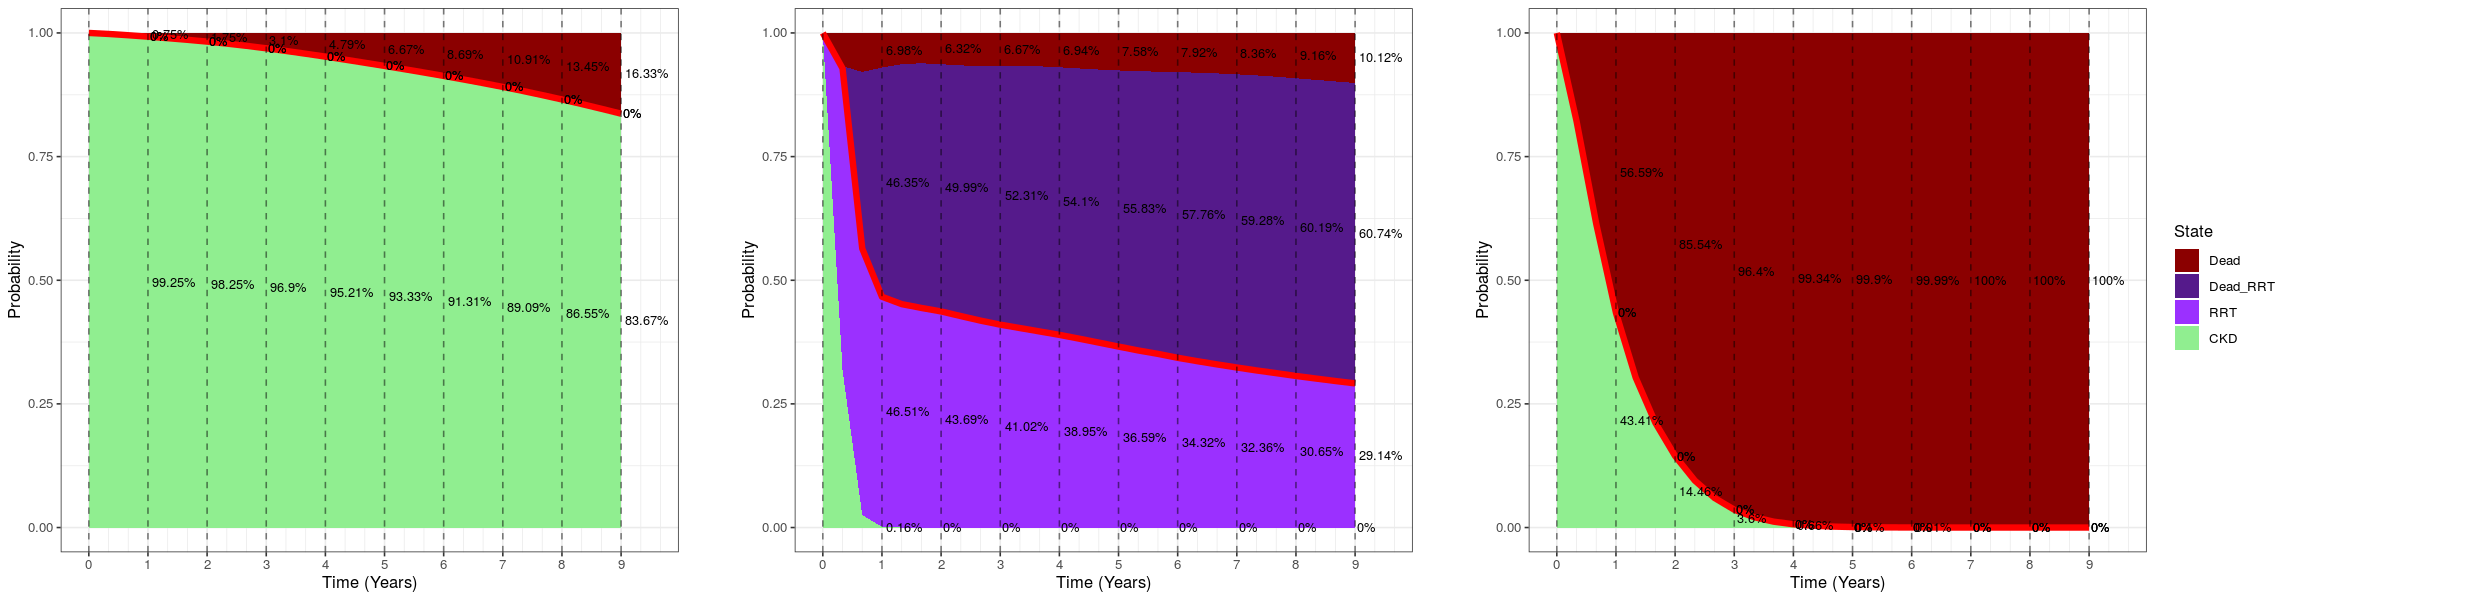
\includegraphics[width=1\linewidth]{figure/Dev_Paper_Example} 

}

\caption{Results of Example Patients}\label{fig:Example-Predictions-trend}
\end{figure}
\hypertarget{calculator-1}{%
\subsection{Calculator}\label{calculator-1}}

The calculator is available online here:

\url{https://michael-barrowman.shinyapps.io/MSCPM_for_CKD_Patients/}.

\hypertarget{discussion-4}{%
\section{Discussion}\label{discussion-4}}

We have used data provided by SKS to develop a Multi-State Clinical Prediction Model and then validated this model within the SKS and SERPR datasets. Within our Models, the cause of a patient's renal disease had the widest effect on patient outcomes meaning that outcomes are highly dependent on ERA-EDTA classification of the diagnosis. Most groupings resulted in a lowered hazard of death and an increased hazard of RRT compared to the baseline of Systemic diseases.

Models performed well in model validation with the Three-State Model slightly out performing the other two models in calibration and overall predictive ability, however the Five-State model performed marginally better in terms of discriminative ability. Both Multi-State Models outperformed the Two-State (Traditional) Model.

The application of a Multi-state clinical prediction model to this field is novel and gives a powerful tool for providing individualised predictions of multiple outcomes at a wide range of time points. The general inclusion criteria for the development dataset, and the wide range of patient ages and measurements allows for the model to be applied to a broad spectrum of patients.

Although the inclusion criteria for SKS were broad, the demographics of the local area resulted in homogeneity of ethnicity, which may create a limitation to the applicability of our model. The Renal Department at SRFT is a tertiary care facility for CKD sufferers and is well renowned for its capabilities of care meaning that it is likely to attract less-healthy patients from a wider catchment area, making the cohort of patients in the development population in worse condition than the general population of CKD patients.

There were also high levels of missingness in the eGFR and uPCR rates of changes would also produce a bias, due to these measures likely being missing not at random. The derivation of the validation dataset ensured that all patients had an eGFR Rate measurement; this was done to avoid data missing not at random (only negative or missing data would be available as patient's eGFR dropped to less than 60), however deriving data in this way could itself induce a survivor bias in the start date used for patients.

In the Five-State Model, We omitted the analysis of the Tx to Dead state due to the anticipated low number of events within the SKS dataset. The lowest number of events for a transition was therefore PD to Dead, which had only 107. Altogether, we considered 26 covariates (with 4 categorical covariates) and so this equates to 36 predictor parameters and an events per predictor parameter (EPP) of 2.97. This is below the recommendations of Riley et al {[}\protect\hyperlink{ref-riley_minimum_2019}{22}{]}, whose calculations produce a requirement of 4.54 EPP. This requirement was also not satisfied by the CKD to PD transition (EPP = 6.36,required = 10.2) or the CKD to Tx transition (EPP = 2.97, required = 17.6). Fortunately, this limitation is confined to the Five-State Model.

We have assumed a proportional hazards relationship between the predictors and probability of survival, which is considered by some to be a strong assumption to make, however we acknowledge this limitation, and the authors believe that it is mitigated by the flexibility that the assumption permits. In addition to the general PH assumption, the R-P model requires the assumption that the log cumulative hazard function follows a cubic spline, (however this is a much weaker assumption {[}\protect\hyperlink{ref-royston_flexible_2002}{112}{]}), which is modelled as part of the regression. We did not assess the viability of these models as it was believed this assumption to make our results more understandable.

Compared to the raw internal validation, the model performance during the external validation was worse for all metrics. However, once adjusted for optimism, the results were much more cohesive which implies that the model is highly transportable to a new population without much alterations being required. Due to the differences in the healthcare systems of England and Scotland, it can be appreciated that despite the populations being similar, their care would be different enough to emphasise a larger difference between our populations than that shown in our (relatively homogeneous) populations.

Although not directly assessing causality in regards to state-transitions, our Three-State model can be used by clinicians to either expedite or delay transition of a patient onto RRT, if it is believed that this would be beneficial. Alternatively, the Five-State Model can be interpreted to provide information regarding \emph{which} treatment might be benficial for a patient.

Our paper has clearly demonstrated the accuracy of such a model. However, further research would be needed to establish the effectiveness and efficacy of its use in clinical practice {[}\protect\hyperlink{ref-moons_prognosis_2009-1}{113}{]} by comparing it to standard care and establishing whether the use of our model improves patient outcomes.

All three models produced for this work performed well in terms of accuracy, calibration and discrimination when applied internally and externally. This shows directly that the models are suitable for use in populations similar to both our development and our validation datasets. It can also be concluded that the models can be transported and applied to any population with a similar healthcare system to the UK.

\hypertarget{chap-conclusion}{%
\chapter{Conclusion}\label{chap-conclusion}}

\chaptermark{Conclusion}

Last updated: 21 Apr

Here is where my concluding section will go.

The end.

\hypertarget{appendix-appendices}{%
\appendix}


\hypertarget{chap-Conf-CR-supp}{%
\chapter{How unmeasured confounding in a competing risks setting can affect treatment effect estimates in observational studies - Supplementary Material}\label{chap-Conf-CR-supp}}

\chaptermark{Competing Risks and Unmeasured Confounding - Supp}

\hypertarget{simulation-details}{%
\section{Simulation Details}\label{simulation-details}}

The populations

\hypertarget{mathematics-of-subdistribution-hazards}{%
\section{Mathematics of Subdistribution Hazards}\label{mathematics-of-subdistribution-hazards}}

Due to the relationship between the cause specific hazard functions and the subdistribution hazard functions they cannot both satisfy the proportional hazards assumption. We have defined CSH functions to be proportio

\hypertarget{chap-IPCW-logistic-supp}{%
\chapter{Inverse Probability Weighting Adjustment of the Logistic Regression Calibration-in-the-Large - Supplementary Material}\label{chap-IPCW-logistic-supp}}

\chaptermark{IPCW Calibration-in-the-Large - Supp}

\hypertarget{calibration-slope}{%
\section{Calibration Slope}\label{calibration-slope}}

The main purpose of this paper was to assess the evaluation of calibration-in-the-large at different time points in a time-to-event clinical prediction model. Along with calibration-in-the-large, various methods of calibration can also produce measures of calibration slope. Calibration slope provides an insight into how well the model predicts outcomes across the range of predictions. In an ideal model, the calibration slope would be 1. The Logistic Weighted, Logistic Unweighted and Pseudo-Observation methods described above can provide estimates of the calibration slope. For each of these methods, we first estimate the calibration-in-the-large as above, using a predictor as an offset, then we use this estimate as an offset to predict the calibration slope (without an intercept term).

\hypertarget{results-6}{%
\subsection{Results}\label{results-6}}

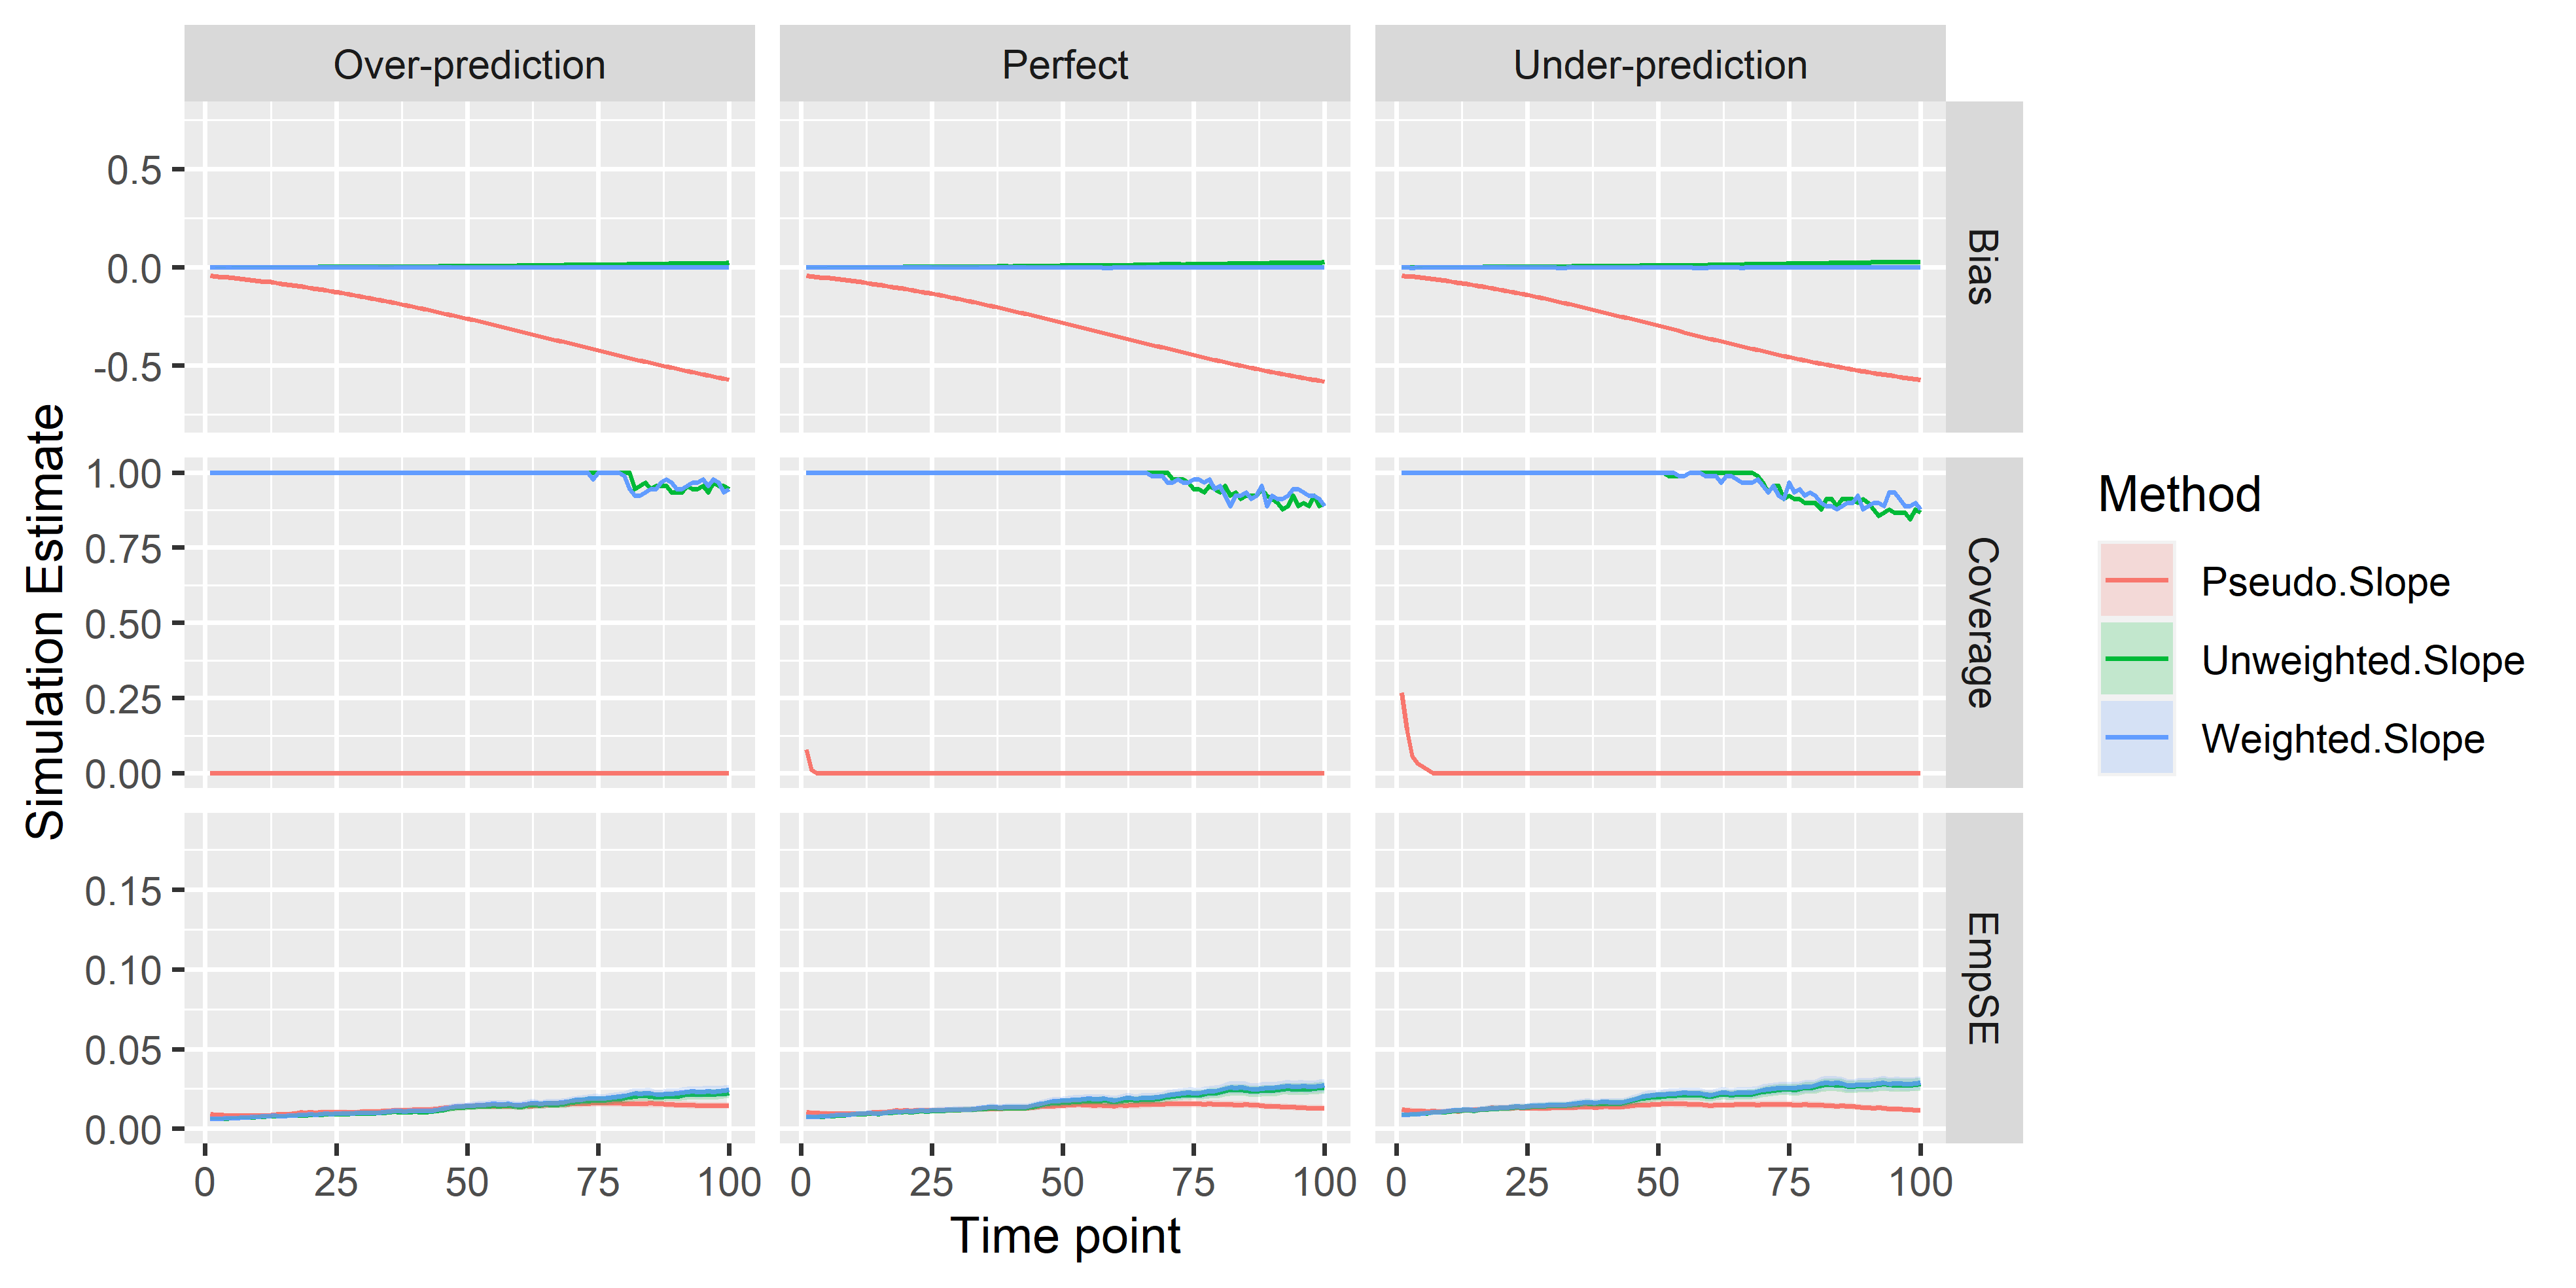
\includegraphics[width=54.68in]{figure/IPCW_Logistic/SlopePlot_b(1)_g(0)_e(0.5)}

Results currently show bias/coverage/EmpsE away from 0, rather than 1. Needs fixing. Oops.

\hypertarget{discussion-5}{%
\subsection{Discussion}\label{discussion-5}}

Brief discussion, much briefer than the main points.

\hypertarget{chap-dev-paper-supp}{%
\chapter{Development and External Validation of a Multi-State Clinical Prediction Model for Chronic Kidney Disease Patients Progressing onto Renal Replacement Therapy and Death - Supplementary Material}\label{chap-dev-paper-supp}}

\chaptermark{Development and Validation of MSCPM - Supp}

\hypertarget{statistical-analysis}{%
\section{Statistical Analysis}\label{statistical-analysis}}

\hypertarget{development}{%
\subsection{Development}\label{development}}

Data was recorded in a time-updated manner, however all variables were measured at baseline to emulate the real-world application of the model (i.e.~future prediction of states and not covariates). Variables considered as covariates were demographics (sex, age, smoking status and alcohol consumption), comorbidities (congestive cardiac failure (CCF), chronic obstructive pulmonary disease (COPD), prior cerebrovascular accident (CVA), hypertension (HT), diabetes mellitus (DM), ischemic heart disease (IHD), chronic liver disease (LD), prior myocardial infarction (MI), peripheral vascular disease (PVD) and slid tumour (ST)), physical parameters (BMI, blood pressure), blood results (haemoglobin, albumin, corrected calcium and phosphate measures), urine protein creatinine ratio (uPCR) and primary renal diagnosis (grouped as per ERA-EDTA classifications {[}\protect\hyperlink{ref-venkat-raman_new_2012}{114}{]}). Ethnicity was assessed in the populations, but as most patients were white, it was omitted as a potential predictor from the models.

uPCR and eGFR Rate of change were also calculated {[}\protect\hyperlink{ref-kovesdy_past_2016}{115}{]}, {[}\protect\hyperlink{ref-naimark_past_2016}{116}{]} as the difference between the two most recent measures divided by time difference in years. \(\textrm{Age}^2\), log(Age), log(eGFR Rate) and log(uPCR Rate) were considered as transformations within the model. log(Calendar Time) was included as a covariate to adjust for secular trends in treatment preferences {[}\protect\hyperlink{ref-bhatnagar_epidemiology_2015}{31}{]}. Calendar Time was defined as length of time between start date and 1st January 2019.

Intermediate states (RRT or modality) were considered to be medically transformative, and so a semi-markov (clock reset) method for analysis was considered to be well justified {[}\protect\hyperlink{ref-meira-machado_multi-state_2009}{117}{]}. Each transition was modelled under a proportional hazards assumption using the Royston-Parmar technique {[}\protect\hyperlink{ref-royston_flexible_2002}{112}{]} to estimate coefficients for each covariate and a restricted cubic spline (on the log-time scale) for the baseline cumulative hazard. The cumulative hazards for each transition can be combined to produce estimates for the probability of a patient being in any state at any time {[}\protect\hyperlink{ref-putter_tutorial_2007}{118}{]}.

For variable selection, we stacked the imputed datasets together to create a larger, pseudo-population {[}\protect\hyperlink{ref-wood_how_2008}{119}{]} and performed backwards-forwards selection based on minimising the AIC at each step. This was repeated for each transition and for different numbers of evenly spaced knots in modelling the form of the baseline hazard, K=\{0,1,2,3,4,5\}. This allowed for different transitions to use different sets of variables and numbers of knots in the final model. Some combinations of variables resulted in models that were intractable and so these models were excluded. Once a set of variables were chosen, the R-P model was applied to each imputed dataset individually and the resulting coefficients and cubic spline parameters were aggregated across imputations using Rubin's Rules {[}\protect\hyperlink{ref-rubin_multiple_1984}{120}{]}. This gave a model fully defined by smooth cubic splines representing the cumulative cause-specific hazard and individualised proportional hazards for each transition.

All missing data were assumed to be missing at random and so were multiply imputed using chained equations with the Nelson-Aalen estimators for each relevant transition as predictors {[}\protect\hyperlink{ref-white_imputing_2009}{121}{]}. Some variables (smoking status and histories of COPD, LD and ST) were present in the SKS (development) dataset, but were completely missing in the SERPR extract (validation) and so these were multiply imputed from the development dataset {[}\protect\hyperlink{ref-janssen_dealing_2009}{122}{]}.

\hypertarget{validation}{%
\subsection{Validation}\label{validation}}

Each of the three models were internally validated in the development dataset using bootstrapping to adjust for optimism and then further externally validated in the validation dataset extracted from SERPR{[}\protect\hyperlink{ref-schomaker_bootstrap_2018}{123}{]}. The bootstrapping method was also used for both validations to produce confidence intervals around the performance metric estimates. To assess the performance in low eGFR patients, the models were also validated in subsets of the SKS and SERPR where patients had an eGFR \textless{} 30/ml/min/1.73m\textsuperscript{2}.

For validation purposes, we consider Death and Death after RRT/HD/PD to be distinct states meaning that for the Three-State model, we have \(K=4\) pathways a patient can take and for the Five-State model, we have \(K=7\). To compare across models, we combined states together to collapse down to simpler versions. We collapsed the Three-State model to a two-state structure by combining the CKD and RRT states into an Alive state. We collapsed the Five-State model to a three-state structure by combining the HD, PD and Tx into an RRT state and then further down to a two-state structure as with the Three-State model. We will report performance measures at 360 days (approx. 1-year), 720 days (approx. 2-years) and 1800 days (approx. 5-years). As well as presenting the performance measures over time.

The performance metrics were chosen from those defined in chapter \ref@(chap-performance-metrics)

The overall accuracy of each model was assessed using the MSM adjusted Brier Score, which is a proper score function {[}\protect\hyperlink{ref-gneiting_strictly_2007}{124}{]} assigning 0 to a non-informative model and 1 to a perfect model, with negative numbers implying the model performs worse than assuming every patient's state predictions are the same as the overall prevalence within the population.

The discrimination of each model was assessed using the MSM extension to the c-statistic {[}\protect\hyperlink{ref-calster_extending_2012-1}{125}{]}. The c-statistic is a score between 0 and 1 with higher scores suggesting a better model and a c-statistic of 0.5 suggesting the model performs no better than a non-informative model.

The calibration of each model was assessed using MSM multinomial logistic regression (MLR) {[}\protect\hyperlink{ref-hoorde_assessing_2014}{126}{]} which extends the logistic regression to three or more mutually exclusive outcomes {[}\protect\hyperlink{ref-riley_prognosis_2019}{6}{]}. This produces an intercept vector of length \(K-1\) and a Slope-matrix of dimension \((K-1) \times (K-1)\). As with the traditional calibration intercept for a well performing model, the MLR intercept values should all be as close to 0 as possible. The traditional calibration slope should be as close to 1 as possible and so the multi-state extension of the slope, the Slope-matrix should be as close to the identity matrix (\(I\)) as possible.

\hypertarget{model-results}{%
\section{Model Results}\label{model-results}}

\hypertarget{two-state-model}{%
\subsection{Two State Model}\label{two-state-model}}

Table \ref{tab:PH-Two} shows the proportional hazard ratios for the transitions in the Two-State Model. Older patients have a higher hazard towards death, low adn decreasing eGFR increased hazard as did a history of diabetes. Patients with a primary renal diagnosis included in the ERA-EDTA {[}\protect\hyperlink{ref-venkat-raman_new_2012}{114}{]} definition of Systemic diseases affecting the kidney had the highest likelihood of death.
\begin{table}[!h]

\caption{\label{tab:PH-Two}{\small Proportional Hazards for each transition in the Two-State Model}}
\centering
\fontsize{7}{9}\selectfont
\begin{tabular}[t]{>{\raggedright\arraybackslash}p{54em}>{\ttfamily\raggedleft\arraybackslash}p{43em}}
\toprule
  & Alive to Dead\\
\midrule
\rowcolor{gray!6}  \addlinespace[0.3em]
\multicolumn{2}{l}{\textbf{Age}}\\
\hspace{1em}(Age-60) & 0.110 (  -0.055,   0.275)\\
\hspace{1em}(Age-60)\textsuperscript{} & -0.000 (  -0.001,   0.000)\\
\rowcolor{gray!6}  \hspace{1em}log(Age) & -2.853 ( -12.306,   6.599)\\
\addlinespace[0.3em]
\multicolumn{2}{l}{\textbf{eGFR}}\\
\hspace{1em}eGFR & -0.013 (  -0.018,  -0.008)\\
\rowcolor{gray!6}  \hspace{1em}eGFR Rate & -0.007 (  -0.090,   0.075)\\
\hspace{1em}log(eGFR Rate) & 0.090 (  -0.199,   0.380)\\
\rowcolor{gray!6}  \addlinespace[0.3em]
\multicolumn{2}{l}{\textbf{uPCR}}\\
\hspace{1em}uPCR & \\
\hspace{1em}uPCR Rate & \\
\rowcolor{gray!6}  \hspace{1em}log(uPCR Rate) & \\
\addlinespace[0.3em]
\multicolumn{2}{l}{\textbf{Measures}}\\
\hspace{1em}SBP & \\
\rowcolor{gray!6}  \hspace{1em}DBP & 0.004 (  -0.000,   0.009)\\
\hspace{1em}BMI & \\
\rowcolor{gray!6}  \hspace{1em}Albumin & -0.048 (  -0.061,  -0.034)\\
\hspace{1em}Corrected Calcium & 0.222 (  -0.153,   0.599)\\
\rowcolor{gray!6}  \hspace{1em}Haemoglobin & -0.011 (  -0.015,  -0.007)\\
\hspace{1em}Phosphate & 0.338 (   0.119,   0.557)\\
\rowcolor{gray!6}  \addlinespace[0.3em]
\multicolumn{2}{l}{\textbf{Gender}}\\
\hspace{1em}Female & -0.172 (  -0.291,  -0.053)\\
\addlinespace[0.3em]
\multicolumn{2}{l}{\textbf{Smoking Status}}\\
\hspace{1em}Former (3 years+) & -0.403 (  -0.908,   0.101)\\
\rowcolor{gray!6}  \hspace{1em}Non-Smoker & -0.226 (  -0.358,  -0.095)\\
\hspace{1em}Smoker & 0.376 (   0.212,   0.539)\\
\rowcolor{gray!6}  \addlinespace[0.3em]
\multicolumn{2}{l}{\textbf{Primary Renal Diagnosis}}\\
\hspace{1em}Familial / hereditary nephropathies & -0.399 (  -0.728,  -0.070)\\
\hspace{1em}Glomerular disease & -0.406 (  -0.618,  -0.193)\\
\rowcolor{gray!6}  \hspace{1em}Miscellaneous renal disorders & -0.220 (  -0.434,  -0.005)\\
\hspace{1em}Tubulointerstitial disease & -0.452 (  -0.696,  -0.208)\\
\rowcolor{gray!6}  \addlinespace[0.3em]
\multicolumn{2}{l}{\textbf{Comorbidity}}\\
\hspace{1em}DM & 0.144 (   0.022,   0.265)\\
\hspace{1em}CCF & -0.378 (  -0.505,  -0.252)\\
\rowcolor{gray!6}  \hspace{1em}MI & -0.165 (  -0.304,  -0.026)\\
\hspace{1em}IHD & 0.070 (  -0.059,   0.200)\\
\rowcolor{gray!6}  \hspace{1em}PVD & -0.240 (  -0.371,  -0.109)\\
\hspace{1em}CVA & -0.128 (  -0.293,   0.036)\\
\rowcolor{gray!6}  \hspace{1em}COPD & -0.203 (  -0.330,  -0.076)\\
\hspace{1em}LD & -0.241 (  -0.573,   0.091)\\
\rowcolor{gray!6}  \hspace{1em}ST & -0.299 (  -0.440,  -0.158)\\
\hspace{1em}HT & -0.080 (  -0.339,   0.177)\\
\bottomrule
\end{tabular}
\end{table}
Equation \eqref{eq:CH-Two-16} below shows the baseline cumulative hazard functions for the transition from Alive to Dead in the Two-State Model.
\begin{equation}
\Lambda_{0,16}(t)=\begin{cases} 1.15764\log(t)+6.17808 & 0 \le t < 3 \\ 0.00075\log(t)^3-0.00247\log(t)^2+1.16036\log(t)+6.17708 & 3 \le t < 520 \\ 0.13983\log(t)^3-2.61165\log(t)^2+17.47602\log(t)-27.83122 & 520 \le t < 984 \\ -0.19361\log(t)^3+4.28227\log(t)^2-30.03426\log(t)+81.30981 & 984 \le t < 1454 \\ -0.15458\log(t)^3+3.42966\log(t)^2-23.82553\log(t)+66.23901 & 1454 \le t < 2009 \\ 0.37097\log(t)^3-8.56171\log(t)^2+67.37553\log(t)-164.97265 & 2009 \le t < 2900 \\ -0.16209\log(t)^3+4.18769\log(t)^2-34.26862\log(t)+105.14551 & 2900 \le t < 5497 \\ 1.79561\log(t)+1.61764)) & 5497 \le t \label{eq:CH-Two-16}\end{cases}
\end{equation}
Table \ref{tab:IV-Two} shows the results from the internal validation in the Two-State Model. Calibration Intercept is close to 0, implying the model is well calibrated overall with a high c-statistic and Brier Score. Calibration Slope above 1 implies that the model under-estimates outcomes.
\begin{table}[!h]

\caption{\label{tab:IV-Two}{\small Internal Validation of the Two-State Model, results presented as Estimate (95\% CI, where possible)}}
\centering
\fontsize{7}{9}\selectfont
\begin{tabular}[t]{>{}l>{}l>{\ttfamily}r>{\ttfamily}r>{\ttfamily}r>{\ttfamily}r}
\toprule
Predicting & eGFR & One Year & Two Year & Five Year & Average\\
\midrule
\rowcolor{gray!6}  \addlinespace[0.3em]
\multicolumn{6}{l}{\textbf{Brier}}\\
\hspace{1em}Two & < 60 & 0.63 ( 0.62,  0.63) & 0.69 ( 0.69,  0.69) & 0.66 ( 0.66,  0.67) & 0.63 ( 0.62,  0.63)\\
\hspace{1em}Two & < 30 & 0.71 ( 0.71,  0.72) & 0.68 ( 0.68,  0.69) & 0.66 ( 0.66,  0.66) & 0.63 ( 0.63,  0.64)\\
\rowcolor{gray!6}  \addlinespace[0.3em]
\multicolumn{6}{l}{\textbf{c-statistic}}\\
\hspace{1em}Two & < 60 & 0.82 ( 0.82,  0.82) & 0.85 ( 0.84,  0.85) & 0.81 ( 0.81,  0.81) & 0.81 ( 0.81,  0.82)\\
\hspace{1em}Two & < 30 & 0.84 ( 0.84,  0.84) & 0.83 ( 0.82,  0.83) & 0.83 ( 0.82,  0.83) & 0.81 ( 0.81,  0.81)\\
\rowcolor{gray!6}  \addlinespace[0.3em]
\multicolumn{6}{l}{\textbf{Intercept}}\\
\hspace{1em}Two & < 60 & 0.01 ( 0.00,  0.01) & 0.01 ( 0.00,  0.01) & -0.02 (-0.02, -0.01) & -0.00 (-0.01, -0.00)\\
\hspace{1em}Two & < 30 & -0.02 (-0.02, -0.02) & 0.00 ( 0.00,  0.01) & 0.00 ( 0.00,  0.01) & -0.00 (-0.00, -0.00)\\
\rowcolor{gray!6}  \addlinespace[0.3em]
\multicolumn{6}{l}{\textbf{Slope}}\\
\hspace{1em}Two & < 60 & \emph{1.33} & \emph{1.46} & \emph{1.26} & \emph{1.48}\\
\hspace{1em}Two & < 30 & \emph{1.23} & \emph{1.25} & \emph{1.30} & \emph{1.51}\\
\bottomrule
\end{tabular}
\end{table}
Table \ref{tab:EV-Two} shows the results from the external validation in the Two-State Model, which shows similar results to the internal validation with slightly impaired perfomance, which is to be expected in an external validation.
\begin{table}[!h]

\caption{\label{tab:EV-Two}{\small External Validation of the Two-State Model, results presented as Estimate (95\% CI, where possible)}}
\centering
\fontsize{7}{9}\selectfont
\begin{tabular}[t]{>{}l>{}l>{\ttfamily}r>{\ttfamily}r>{\ttfamily}r>{\ttfamily}r}
\toprule
Predicting & eGFR & One Year & Two Year & Five Year & Average\\
\midrule
\rowcolor{gray!6}  \addlinespace[0.3em]
\multicolumn{6}{l}{\textbf{Brier}}\\
\hspace{1em}Two & < 60 & 0.64 ( 0.63,  0.64) & 0.57 ( 0.56,  0.57) & 0.57 ( 0.56,  0.58) & 0.56 ( 0.56,  0.57)\\
\hspace{1em}Two & < 30 & 0.67 ( 0.66,  0.67) & 0.64 ( 0.63,  0.64) & 0.57 ( 0.56,  0.57) & 0.57 ( 0.56,  0.57)\\
\rowcolor{gray!6}  \addlinespace[0.3em]
\multicolumn{6}{l}{\textbf{c-statistic}}\\
\hspace{1em}Two & < 60 & 0.81 ( 0.81,  0.82) & 0.81 ( 0.80,  0.81) & 0.80 ( 0.79,  0.80) & 0.78 ( 0.78,  0.78)\\
\hspace{1em}Two & < 30 & 0.81 ( 0.81,  0.81) & 0.80 ( 0.80,  0.81) & 0.78 ( 0.78,  0.79) & 0.78 ( 0.78,  0.78)\\
\rowcolor{gray!6}  \addlinespace[0.3em]
\multicolumn{6}{l}{\textbf{Intercept}}\\
\hspace{1em}Two & < 60 & -0.00 (-0.00,  0.00) & 0.02 ( 0.01,  0.02) & 0.00 ( 0.00,  0.01) & -0.00 (-0.00,  0.00)\\
\hspace{1em}Two & < 30 & 0.02 ( 0.01,  0.02) & -0.05 (-0.05, -0.04) & 0.01 ( 0.01,  0.02) & -0.00 (-0.00,  0.00)\\
\rowcolor{gray!6}  \addlinespace[0.3em]
\multicolumn{6}{l}{\textbf{Slope}}\\
\hspace{1em}Two & < 60 & \emph{1.29} & \emph{1.25} & \emph{1.72} & \emph{2.21}\\
\hspace{1em}Two & < 30 & \emph{1.37} & \emph{1.37} & \emph{2.05} & \emph{1.88}\\
\bottomrule
\end{tabular}
\end{table}
\hypertarget{three-state-model}{%
\subsection{Three State Model}\label{three-state-model}}

In the Three-State Model, older patients are predicted to be likely to transition to RRT. Increased rates of decline of eGFR were associated with the transition from CKD to RRT. The full results are shown in table \ref{tab:PH-Three}.

\newgeometry{margin=2cm}
\begin{landscape}\begin{table}

\caption{\label{tab:PH-Three}{\small Proportional Hazards for each transition in the Three-State Model}}
\centering
\fontsize{7}{9}\selectfont
\begin{tabular}[t]{>{\raggedright\arraybackslash}p{54em}>{\ttfamily\raggedleft\arraybackslash}p{43em}>{\ttfamily\raggedleft\arraybackslash}p{43em}>{\ttfamily\raggedleft\arraybackslash}p{43em}}
\toprule
  & CKD to Dead & CKD to RRT & RRT to Dead\\
\midrule
\rowcolor{gray!6}  \addlinespace[0.3em]
\multicolumn{4}{l}{\textbf{Age}}\\
\hspace{1em}(Age-60) & 0.161 (  -0.051,   0.374) & -0.041 (  -0.051,  -0.031) & 0.063 (   0.050,   0.076)\\
\hspace{1em}(Age-60)\textsuperscript{} & -0.000 (  -0.002,   0.000) & -0.000 (  -0.000,  -0.000) & \\
\rowcolor{gray!6}  \hspace{1em}log(Age) & -5.725 ( -17.969,   6.518) &  & \\
\addlinespace[0.3em]
\multicolumn{4}{l}{\textbf{eGFR}}\\
\hspace{1em}eGFR & -0.013 (  -0.019,  -0.006) & -0.095 (  -0.108,  -0.082) & 0.011 (  -0.001,   0.025)\\
\rowcolor{gray!6}  \hspace{1em}eGFR Rate &  & 0.055 (  -0.021,   0.131) & -0.056 (  -0.363,   0.250)\\
\hspace{1em}log(eGFR Rate) & 0.042 (  -0.125,   0.210) &  & 0.227 (  -0.770,   1.225)\\
\rowcolor{gray!6}  \addlinespace[0.3em]
\multicolumn{4}{l}{\textbf{uPCR}}\\
\hspace{1em}uPCR & 0.125 (  -0.318,   0.569) & 0.700 (   0.112,   1.288) & -0.108 (  -0.736,   0.519)\\
\hspace{1em}uPCR Rate &  & -0.019 (  -0.045,   0.005) & 0.036 (  -0.062,   0.136)\\
\rowcolor{gray!6}  \hspace{1em}log(uPCR Rate) &  & 0.218 (  -0.310,   0.747) & -0.198 (  -0.534,   0.137)\\
\addlinespace[0.3em]
\multicolumn{4}{l}{\textbf{Measures}}\\
\hspace{1em}SBP & -0.001 (  -0.004,   0.002) & 0.005 (  -0.000,   0.011) & \\
\rowcolor{gray!6}  \hspace{1em}DBP & 0.006 (   0.000,   0.013) & 0.006 (  -0.001,   0.015) & \\
\hspace{1em}BMI &  &  & \\
\rowcolor{gray!6}  \hspace{1em}Albumin & -0.044 (  -0.064,  -0.024) & -0.032 (  -0.059,  -0.004) & -0.044 (  -0.079,  -0.009)\\
\hspace{1em}Corrected Calcium & 0.280 (  -0.192,   0.752) & -0.515 (  -1.207,   0.177) & \\
\rowcolor{gray!6}  \hspace{1em}Haemoglobin & -0.013 (  -0.017,  -0.008) & -0.005 (  -0.012,   0.001) & -0.005 (  -0.014,   0.003)\\
\hspace{1em}Phosphate & 0.511 (   0.132,   0.890) & 0.869 (  -0.059,   1.799) & \\
\rowcolor{gray!6}  \addlinespace[0.3em]
\multicolumn{4}{l}{\textbf{Gender}}\\
\hspace{1em}Female & -0.235 (  -0.371,  -0.099) & -0.277 (  -0.455,  -0.099) & \\
\addlinespace[0.3em]
\multicolumn{4}{l}{\textbf{Smoking Status}}\\
\hspace{1em}Former (3 years+) & -0.212 (  -0.879,   0.453) & -0.133 (  -0.757,   0.490) & -0.282 (  -1.082,   0.518)\\
\rowcolor{gray!6}  \hspace{1em}Non-Smoker & -0.198 (  -0.345,  -0.051) & -0.162 (  -0.364,   0.039) & -0.294 (  -0.598,   0.009)\\
\hspace{1em}Smoker & 0.356 (   0.160,   0.551) & 0.175 (  -0.076,   0.428) & 0.387 (   0.068,   0.706)\\
\rowcolor{gray!6}  \addlinespace[0.3em]
\multicolumn{4}{l}{\textbf{Primary Renal Diagnosis}}\\
\hspace{1em}Familial / hereditary nephropathies & -0.424 (  -0.854,   0.006) & 1.029 (   0.720,   1.338) & -0.562 (  -1.084,  -0.040)\\
\hspace{1em}Glomerular disease & -0.394 (  -0.635,  -0.154) & -0.165 (  -0.465,   0.134) & -0.488 (  -0.883,  -0.094)\\
\rowcolor{gray!6}  \hspace{1em}Miscellaneous renal disorders & -0.263 (  -0.505,  -0.021) & -0.649 (  -1.143,  -0.155) & 0.033 (  -0.553,   0.620)\\
\hspace{1em}Tubulointerstitial disease & -0.463 (  -0.741,  -0.184) & -0.265 (  -0.577,   0.046) & -0.310 (  -0.803,   0.181)\\
\rowcolor{gray!6}  \addlinespace[0.3em]
\multicolumn{4}{l}{\textbf{Comorbidity}}\\
\hspace{1em}DM & 0.122 (  -0.011,   0.255) & 0.141 (  -0.074,   0.358) & 0.200 (  -0.096,   0.496)\\
\hspace{1em}CCF & -0.394 (  -0.535,  -0.253) &  & -0.299 (  -0.597,  -0.002)\\
\rowcolor{gray!6}  \hspace{1em}MI & -0.246 (  -0.397,  -0.094) & 0.234 (  -0.061,   0.530) & 0.186 (  -0.199,   0.572)\\
\hspace{1em}IHD & 0.102 (  -0.041,   0.245) & -0.077 (  -0.334,   0.179) & -0.097 (  -0.424,   0.228)\\
\rowcolor{gray!6}  \hspace{1em}PVD & -0.248 (  -0.394,  -0.103) & -0.168 (  -0.405,   0.068) & -0.183 (  -0.492,   0.126)\\
\hspace{1em}CVA & -0.070 (  -0.252,   0.111) &  & -0.168 (  -0.577,   0.240)\\
\rowcolor{gray!6}  \hspace{1em}COPD & -0.289 (  -0.433,  -0.145) &  & \\
\hspace{1em}LD & -0.169 (  -0.578,   0.239) & -0.316 (  -0.731,   0.097) & -0.270 (  -0.858,   0.318)\\
\rowcolor{gray!6}  \hspace{1em}ST & -0.274 (  -0.431,  -0.117) & -0.181 (  -0.516,   0.153) & -0.278 (  -0.611,   0.055)\\
\hspace{1em}HT &  & 0.274 (  -0.176,   0.726) & -0.416 (  -1.104,   0.271)\\
\bottomrule
\end{tabular}
\end{table}
\end{landscape}
\restoregeometry

Female patients are predicted to be more likely to remain in the CKD state than Males, or to remain in the RRT state once there. Smokers were predicted as more likely than Non-/Former Smokers to undergo any transition, apart from CKD to Tx. Blood results had associations with all transitions in some way, and disease etiology were strongly associated with the transitions giving a wide range of predictions.

The equations \eqref{eq:CH-Three-16}, \eqref{eq:CH-Three-15} and \eqref{eq:CH-Three-56} shows the baseline cumulative hazard functions for the transition from CKD to Dead, CKD to RRT and RRT to Dead, respectively in the Three-State Model.
\begin{equation}
\Lambda_{0,16}(t)=\begin{cases} 1.19795\log(t)+17.68798 & 0 \le t < 3 \\ -9e-05\log(t)^3+3e-04\log(t)^2+1.19761\log(t)+17.68811 & 3 \le t < 443 \\ 0.15869\log(t)^3-2.9019\log(t)^2+18.88018\log(t)-18.22403 & 443 \le t < 873 \\ -0.30096\log(t)^3+6.43659\log(t)^2-44.36299\log(t)+124.54338 & 873 \le t < 1295 \\ -0.04158\log(t)^3+0.86028\log(t)^2-4.40166\log(t)+29.08554 & 1295 \le t < 1876 \\ 0.51263\log(t)^3-11.67048\log(t)^2+90.03919\log(t)-208.17245 & 1876 \le t < 2738 \\ -0.23992\log(t)^3+6.19863\log(t)^2-51.3924\log(t)+164.96467 & 2738 \le t < 5497 \\ 1.98997\log(t)+11.72244)) & 5497 \le t \label{eq:CH-Three-16}\end{cases}
\end{equation}
\begin{equation}
\Lambda_{0,15}(t)=\begin{cases} 1.55753\log(t)-5.44635 & 0 \le t < 18 \\ -0.00279\log(t)^3+0.0242\log(t)^2+1.48757\log(t)-5.37894 & 18 \le t < 270 \\ -0.13576\log(t)^3+2.25776\log(t)^2-11.01817\log(t)+17.96111 & 270 \le t < 538 \\ 0.49133\log(t)^3-9.57146\log(t)^2+63.36209\log(t)-137.93609 & 538 \le t < 919 \\ -0.76978\log(t)^3+16.24541\log(t)^2-112.80782\log(t)+262.78176 & 919 \le t < 1316 \\ 0.30039\log(t)^3-6.81452\log(t)^2+52.82254\log(t)-133.77073 & 1316 \le t < 2000 \\ -0.0123\log(t)^3+0.31552\log(t)^2-1.37092\log(t)+3.53243 & 2000 \le t < 5173 \\ 1.32717\log(t)-4.15818)) & 5173 \le t \label{eq:CH-Three-15}\end{cases}
\end{equation}
\begin{equation}
\Lambda_{0,56}(t)=\begin{cases} 1.35522\log(t)-7.7618 & 0 \le t < 8 \\ -0.01704\log(t)^3+0.1063\log(t)^2+1.13417\log(t)-7.60859 & 8 \le t < 196 \\ 0.21761\log(t)^3-3.6103\log(t)^2+20.75671\log(t)-42.14228 & 196 \le t < 506 \\ -0.67558\log(t)^3+13.07415\log(t)^2-83.12956\log(t)+173.47479 & 506 \le t < 816 \\ 0.8043\log(t)^3-16.69103\log(t)^2+116.42771\log(t)-272.49495 & 816 \le t < 1388 \\ -1.26732\log(t)^3+28.27738\log(t)^2-208.94656\log(t)+512.26643 & 1388 \le t < 1927 \\ 0.17019\log(t)^3-4.34244\log(t)^2+37.78861\log(t)-109.83234 & 1927 \le t < 4940 \\ 0.85568\log(t)-5.12598)) & 4940 \le t \label{eq:CH-Three-56}\end{cases}
\end{equation}
Table \ref{tab:IV-Three} shows the results from the internal validation in the Three-State Model. Performance was overall slightly better in patients in the \textless60 eGFR group than in the \textless30 eGFR group. All measures degraded over time, but the average scores remained strong.
\begin{table}[!h]

\caption{\label{tab:IV-Three}{\small Internal Validation of the Three-State Model, results presented as Estimate (95\% CI, where possible)}}
\centering
\fontsize{7}{9}\selectfont
\begin{tabular}[t]{>{}l>{}l>{\ttfamily}r>{\ttfamily}r>{\ttfamily}r>{\ttfamily}r}
\toprule
Predicting & eGFR & One Year & Two Year & Five Year & Average\\
\midrule
\rowcolor{gray!6}  \addlinespace[0.3em]
\multicolumn{6}{l}{\textbf{Brier}}\\
\hspace{1em}Three & < 60 & 0.74 ( 0.74,  0.75) & 0.68 ( 0.68,  0.69) & 0.64 ( 0.64,  0.65) & 0.67 ( 0.67,  0.68)\\
\hspace{1em}Three & < 30 & 0.75 ( 0.74,  0.75) & 0.73 ( 0.73,  0.73) & 0.68 ( 0.67,  0.68) & 0.68 ( 0.67,  0.68)\\
\rowcolor{gray!6}  \hspace{1em}Two & < 60 & 0.75 ( 0.75,  0.75) & 0.75 ( 0.75,  0.76) & 0.67 ( 0.67,  0.67) & 0.67 ( 0.67,  0.68)\\
\hspace{1em}Two & < 30 & 0.71 ( 0.71,  0.72) & 0.72 ( 0.72,  0.73) & 0.65 ( 0.65,  0.66) & 0.67 ( 0.67,  0.68)\\
\rowcolor{gray!6}  \addlinespace[0.3em]
\multicolumn{6}{l}{\textbf{c-statistic}}\\
\hspace{1em}Three & < 60 & 0.87 ( 0.87,  0.87) & 0.84 ( 0.84,  0.85) & 0.84 ( 0.84,  0.84) & 0.83 ( 0.83,  0.84)\\
\hspace{1em}Three & < 30 & 0.87 ( 0.86,  0.87) & 0.84 ( 0.84,  0.84) & 0.84 ( 0.84,  0.84) & 0.83 ( 0.83,  0.84)\\
\rowcolor{gray!6}  \hspace{1em}Two & < 60 & 0.86 ( 0.86,  0.86) & 0.86 ( 0.86,  0.86) & 0.83 ( 0.83,  0.84) & 0.83 ( 0.83,  0.84)\\
\hspace{1em}Two & < 30 & 0.86 ( 0.85,  0.86) & 0.86 ( 0.85,  0.86) & 0.85 ( 0.85,  0.85) & 0.84 ( 0.83,  0.84)\\
\rowcolor{gray!6}  \addlinespace[0.3em]
\multicolumn{6}{l}{\textbf{Intercept}}\\
\hspace{1em}Three & < 60 & \makecell[r]{-0.00 (-0.00,  0.00)\\  0.00 ( 0.00,  0.01)\\  0.00 ( 0.00,  0.00)} & \makecell[r]{0.00 (-0.00,  0.00)\\ -0.01 (-0.02, -0.01)\\  0.00 ( 0.00,  0.00)} & \makecell[r]{-0.02 (-0.02, -0.01)\\ -0.01 (-0.02, -0.01)\\ -0.00 (-0.01, -0.00)} & \makecell[r]{0.00 ( 0.00,  0.00)\\  0.00 (-0.00,  0.00)\\  0.00 (-0.00,  0.00)}\\
\hspace{1em}Three & < 30 & \makecell[r]{-0.01 (-0.01, -0.01)\\ -0.00 (-0.00, -0.00)\\  0.00 (-0.00,  0.00)} & \makecell[r]{0.00 (-0.00,  0.00)\\ -0.01 (-0.01, -0.00)\\  0.03 ( 0.02,  0.03)} & \makecell[r]{-0.02 (-0.02, -0.01)\\  0.00 (-0.00,  0.00)\\ -0.00 (-0.01, -0.00)} & \makecell[r]{0.00 (-0.00,  0.00)\\  0.00 (-0.00,  0.00)\\  0.00 (-0.00,  0.00)}\\
\rowcolor{gray!6}  \hspace{1em}Two & < 60 & -0.00 (-0.01, -0.00) & 0.02 ( 0.01,  0.02) & 0.00 (-0.00,  0.00) & -0.00 (-0.00,  0.00)\\
\hspace{1em}Two & < 30 & -0.00 (-0.00,  0.00) & -0.04 (-0.04, -0.04) & 0.00 ( 0.00,  0.01) & -0.00 (-0.00,  0.00)\\
\rowcolor{gray!6}  \addlinespace[0.3em]
\multicolumn{6}{l}{\textbf{Slope}}\\
\hspace{1em}Three & < 60 & \makecell[r]{\emph{1.25},  0.00,  0.04\\ -0.03,  \emph{1.10}, -0.00\\ -0.00,  0.01,  \emph{1.16}} & \makecell[r]{\emph{1.17}, -0.06,  0.01\\  0.03,  \emph{1.25}, -0.01\\ -0.01,  0.01,  \emph{1.37}} & \makecell[r]{\emph{1.21}, -0.02, -0.01\\  0.01,  \emph{1.44}, -0.04\\ -0.02,  0.02,  \emph{1.27}} & \makecell[r]{\emph{1.32}, -0.01,  0.00\\ -0.00,  \emph{1.37}, -0.01\\ -0.00,  0.00,  \emph{1.33}}\\
\hspace{1em}Three & < 30 & \makecell[r]{\emph{1.21},  0.02,  0.07\\ -0.04,  \emph{1.24},  0.07\\  0.01,  0.01,  \emph{1.16}} & \makecell[r]{\emph{1.36}, -0.00, -0.01\\  0.00,  \emph{1.31},  0.03\\ -0.02, -0.00,  \emph{1.26}} & \makecell[r]{\emph{1.35}, -0.04, -0.01\\  0.04,  \emph{1.33},  0.04\\  0.04, -0.02,  \emph{1.34}} & \makecell[r]{\emph{1.31},  0.00,  0.00\\ -0.01,  \emph{1.33},  0.01\\ -0.00,  0.00,  \emph{1.35}}\\
\rowcolor{gray!6}  \hspace{1em}Two & < 60 & \emph{1.21} & \emph{1.28} & \emph{1.27} & \emph{1.31}\\
\hspace{1em}Two & < 30 & \emph{1.05} & \emph{1.21} & \emph{1.21} & \emph{1.34}\\
\bottomrule
\end{tabular}
\end{table}
Table \ref{tab:EV-Three} shows the results from the external validation in the Three-State Model.
\begin{table}[!h]

\caption{\label{tab:EV-Three}{\small External Validation of the Three-State Model, results presented as Estimate (95\% CI, where possible)}}
\centering
\fontsize{7}{9}\selectfont
\begin{tabular}[t]{>{}l>{}l>{\ttfamily}r>{\ttfamily}r>{\ttfamily}r>{\ttfamily}r}
\toprule
Predicting & eGFR & One Year & Two Year & Five Year & Average\\
\midrule
\rowcolor{gray!6}  \addlinespace[0.3em]
\multicolumn{6}{l}{\textbf{Brier}}\\
\hspace{1em}Three & < 60 & 0.69 ( 0.68,  0.69) & 0.70 ( 0.69,  0.70) & 0.61 ( 0.60,  0.61) & 0.62 ( 0.62,  0.63)\\
\hspace{1em}Three & < 30 & 0.68 ( 0.67,  0.68) & 0.72 ( 0.71,  0.72) & 0.65 ( 0.64,  0.65) & 0.63 ( 0.62,  0.63)\\
\rowcolor{gray!6}  \hspace{1em}Two & < 60 & 0.67 ( 0.67,  0.67) & 0.70 ( 0.69,  0.70) & 0.63 ( 0.63,  0.63) & 0.62 ( 0.62,  0.63)\\
\hspace{1em}Two & < 30 & 0.66 ( 0.66,  0.67) & 0.70 ( 0.70,  0.70) & 0.65 ( 0.65,  0.66) & 0.63 ( 0.62,  0.63)\\
\rowcolor{gray!6}  \addlinespace[0.3em]
\multicolumn{6}{l}{\textbf{c-statistic}}\\
\hspace{1em}Three & < 60 & 0.82 ( 0.82,  0.82) & 0.83 ( 0.83,  0.83) & 0.79 ( 0.79,  0.79) & 0.81 ( 0.80,  0.81)\\
\hspace{1em}Three & < 30 & 0.85 ( 0.84,  0.85) & 0.84 ( 0.84,  0.84) & 0.83 ( 0.83,  0.83) & 0.81 ( 0.81,  0.81)\\
\rowcolor{gray!6}  \hspace{1em}Two & < 60 & 0.85 ( 0.85,  0.86) & 0.84 ( 0.84,  0.85) & 0.80 ( 0.80,  0.80) & 0.81 ( 0.80,  0.81)\\
\hspace{1em}Two & < 30 & 0.83 ( 0.83,  0.83) & 0.82 ( 0.82,  0.82) & 0.80 ( 0.80,  0.81) & 0.81 ( 0.81,  0.81)\\
\rowcolor{gray!6}  \addlinespace[0.3em]
\multicolumn{6}{l}{\textbf{Intercept}}\\
\hspace{1em}Three & < 60 & \makecell[r]{0.00 (-0.00,  0.00)\\  0.00 ( 0.00,  0.00)\\ -0.00 (-0.00, -0.00)} & \makecell[r]{0.01 ( 0.01,  0.02)\\ -0.01 (-0.01, -0.00)\\  0.00 ( 0.00,  0.01)} & \makecell[r]{0.05 ( 0.04,  0.05)\\  0.01 ( 0.00,  0.01)\\  0.00 ( 0.00,  0.00)} & \makecell[r]{-0.00 (-0.00,  0.00)\\ -0.00 (-0.00,  0.00)\\  0.00 ( 0.00,  0.01)}\\
\hspace{1em}Three & < 30 & \makecell[r]{0.04 ( 0.04,  0.05)\\  0.01 ( 0.00,  0.01)\\  0.00 ( 0.00,  0.01)} & \makecell[r]{0.02 ( 0.01,  0.02)\\ -0.00 (-0.00,  0.00)\\  0.01 ( 0.01,  0.02)} & \makecell[r]{0.01 ( 0.01,  0.01)\\ -0.00 (-0.00,  0.00)\\  0.00 ( 0.00,  0.01)} & \makecell[r]{0.00 (-0.00,  0.00)\\  0.00 (-0.00,  0.00)\\ -0.00 (-0.00,  0.00)}\\
\rowcolor{gray!6}  \hspace{1em}Two & < 60 & 0.00 (-0.00,  0.00) & -0.05 (-0.05, -0.04) & 0.01 ( 0.01,  0.02) & -0.00 (-0.00,  0.00)\\
\hspace{1em}Two & < 30 & 0.02 ( 0.01,  0.02) & -0.00 (-0.00,  0.00) & 0.01 ( 0.00,  0.01) & -0.00 (-0.00,  0.00)\\
\rowcolor{gray!6}  \addlinespace[0.3em]
\multicolumn{6}{l}{\textbf{Slope}}\\
\hspace{1em}Three & < 60 & \makecell[r]{\emph{1.35}, -0.04,  0.04\\  0.06,  \emph{1.49}, -0.03\\  0.01,  0.00,  \emph{1.25}} & \makecell[r]{\emph{1.13}, -0.00,  0.08\\ -0.02,  \emph{1.31},  0.01\\ -0.03,  0.01,  \emph{1.39}} & \makecell[r]{\emph{1.45}, -0.02,  0.03\\  0.03,  \emph{1.73},  0.03\\  0.04, -0.00,  \emph{1.47}} & \makecell[r]{\emph{1.54},  0.00, -0.00\\  0.01,  \emph{1.52},  0.00\\ -0.00,  0.00,  \emph{1.54}}\\
\hspace{1em}Three & < 30 & \makecell[r]{\emph{1.23},  0.03,  0.00\\ -0.05,  \emph{1.20}, -0.04\\ -0.00, -0.00,  \emph{1.37}} & \makecell[r]{\emph{0.99}, -0.01, -0.00\\  0.04,  \emph{1.34}, -0.03\\  0.00,  0.01,  \emph{1.46}} & \makecell[r]{\emph{1.56},  0.00,  0.00\\ -0.05,  \emph{1.49},  0.03\\  0.03,  0.01,  \emph{1.63}} & \makecell[r]{\emph{1.62}, -0.01,  0.01\\ -0.00,  \emph{1.53},  0.01\\  0.00, -0.00,  \emph{1.58}}\\
\rowcolor{gray!6}  \hspace{1em}Two & < 60 & \emph{1.28} & \emph{1.26} & \emph{1.64} & \emph{1.51}\\
\hspace{1em}Two & < 30 & \emph{1.18} & \emph{1.25} & \emph{1.57} & \emph{1.59}\\
\bottomrule
\end{tabular}
\end{table}
\hypertarget{five-state-model}{%
\subsection{Five State Model}\label{five-state-model}}

Table \ref{tab:PH-Five} shows the proportional hazard ratios for the transitions in the Five-State Model.

\newgeometry{margin=2cm}
\begin{landscape}\begin{table}

\caption{\label{tab:PH-Five}{\small Proportional Hazards for each transition in the Five-State Model}}
\centering
\fontsize{7}{9}\selectfont
\begin{tabular}[t]{>{\raggedright\arraybackslash}p{54em}>{\ttfamily\raggedleft\arraybackslash}p{43em}>{\ttfamily\raggedleft\arraybackslash}p{43em}>{\ttfamily\raggedleft\arraybackslash}p{43em}>{\ttfamily\raggedleft\arraybackslash}p{43em}>{\ttfamily\raggedleft\arraybackslash}p{43em}>{\ttfamily\raggedleft\arraybackslash}p{43em}}
\toprule
  & CKD to Dead & CKD to HD & CKD to PD & CKD to Tx & HD to Dead & PD to Dead\\
\midrule
\rowcolor{gray!6}  \addlinespace[0.3em]
\multicolumn{7}{l}{\textbf{Age}}\\
\hspace{1em}(Age-60) & 0.161 (  -0.051,   0.374) & -0.029 (  -0.047,  -0.011) & -0.037 (  -0.057,  -0.018) & -0.099 (  -0.127,  -0.072) & 0.069 (   0.051,   0.087) & 0.046 (   0.024,   0.068)\\
\hspace{1em}(Age-60)\textsuperscript{} & -0.000 (  -0.002,   0.000) & -0.000 (  -0.001,   0.000) & -0.000 (  -0.000,   0.000) & -0.000 (  -0.001,  -0.000) &  & \\
\rowcolor{gray!6}  \hspace{1em}log(Age) & -5.725 ( -17.969,   6.518) &  &  &  &  & \\
\addlinespace[0.3em]
\multicolumn{7}{l}{\textbf{eGFR}}\\
\hspace{1em}eGFR & -0.013 (  -0.019,  -0.006) & -0.088 (  -0.105,  -0.071) & -0.112 (  -0.135,  -0.090) & -0.097 (  -0.120,  -0.074) & 0.016 (   0.000,   0.032) & -0.006 (  -0.036,   0.023)\\
\rowcolor{gray!6}  \hspace{1em}eGFR Rate &  & 0.085 (  -0.058,   0.229) &  & -0.169 (  -0.813,   0.474) & -0.053 (  -0.701,   0.593) & 0.000 (  -0.294,   0.294)\\
\hspace{1em}log(eGFR Rate) & 0.042 (  -0.125,   0.210) & -0.261 (  -0.798,   0.276) & 0.445 (  -0.280,   1.171) & 0.440 (  -1.371,   2.252) & 0.366 (  -1.344,   2.077) & \\
\rowcolor{gray!6}  \addlinespace[0.3em]
\multicolumn{7}{l}{\textbf{uPCR}}\\
\hspace{1em}uPCR & 0.125 (  -0.318,   0.569) & 0.738 (   0.024,   1.451) & 0.650 (  -0.906,   2.207) & 0.317 (  -0.606,   1.241) & -0.577 (  -1.317,   0.162) & 0.071 (  -1.109,   1.251)\\
\hspace{1em}uPCR Rate &  &  & -0.042 (  -0.139,   0.055) & 0.020 (  -0.050,   0.091) & 0.030 (  -0.039,   0.099) & \\
\rowcolor{gray!6}  \hspace{1em}log(uPCR Rate) &  & -0.097 (  -0.880,   0.685) & 0.740 (  -0.470,   1.950) & -0.244 (  -0.940,   0.450) &  & -0.080 (  -0.515,   0.354)\\
\addlinespace[0.3em]
\multicolumn{7}{l}{\textbf{Measures}}\\
\hspace{1em}SBP & -0.001 (  -0.004,   0.002) & 0.003 (  -0.003,   0.010) & 0.009 (  -0.001,   0.020) &  &  & \\
\rowcolor{gray!6}  \hspace{1em}DBP & 0.006 (   0.000,   0.013) & 0.007 (  -0.005,   0.021) & 0.007 (  -0.010,   0.025) &  &  & \\
\hspace{1em}BMI &  & 0.003 (  -0.063,   0.070) &  & -0.019 (  -0.060,   0.021) &  & \\
\rowcolor{gray!6}  \hspace{1em}Albumin & -0.044 (  -0.064,  -0.024) & -0.040 (  -0.075,  -0.005) & -0.037 (  -0.100,   0.025) &  & -0.050 (  -0.096,  -0.003) & -0.021 (  -0.076,   0.032)\\
\hspace{1em}Corrected Calcium & 0.280 (  -0.192,   0.752) &  & -1.291 (  -2.494,  -0.089) &  &  & 1.243 (  -0.187,   2.674)\\
\rowcolor{gray!6}  \hspace{1em}Haemoglobin & -0.013 (  -0.017,  -0.008) & -0.009 (  -0.018,  -0.000) & -0.001 (  -0.016,   0.013) & -0.003 (  -0.016,   0.010) & -0.006 (  -0.017,   0.005) & -0.022 (  -0.037,  -0.006)\\
\hspace{1em}Phosphate & 0.511 (   0.132,   0.890) & 0.904 (   0.087,   1.721) & 1.042 (  -0.336,   2.421) & 0.578 (  -0.333,   1.491) &  & \\
\rowcolor{gray!6}  \addlinespace[0.3em]
\multicolumn{7}{l}{\textbf{Gender}}\\
\hspace{1em}Female & -0.235 (  -0.371,  -0.099) & -0.492 (  -0.754,  -0.230) & -0.156 (  -0.466,   0.154) &  &  & \\
\addlinespace[0.3em]
\multicolumn{7}{l}{\textbf{Smoking Status}}\\
\hspace{1em}Former (3 years+) & -0.212 (  -0.879,   0.453) & -0.121 (  -1.020,   0.776) & -0.337 (  -1.527,   0.851) & 0.599 (  -0.501,   1.701) & -0.519 (  -1.745,   0.706) & -0.026 (  -1.302,   1.249)\\
\rowcolor{gray!6}  \hspace{1em}Non-Smoker & -0.198 (  -0.345,  -0.051) & -0.168 (  -0.567,   0.230) & -0.056 (  -0.405,   0.291) & -0.161 (  -0.623,   0.299) & -0.192 (  -0.641,   0.256) & -0.481 (  -1.013,   0.049)\\
\hspace{1em}Smoker & 0.356 (   0.160,   0.551) & 0.259 (  -0.091,   0.611) & 0.374 (  -0.004,   0.753) & -0.532 (  -1.202,   0.136) & 0.686 (   0.252,   1.120) & 0.136 (  -0.400,   0.674)\\
\rowcolor{gray!6}  \addlinespace[0.3em]
\multicolumn{7}{l}{\textbf{Primary Renal Diagnosis}}\\
\hspace{1em}Familial / hereditary nephropathies & -0.424 (  -0.854,   0.006) & 0.869 (   0.391,   1.348) & 0.982 (   0.466,   1.498) & 1.330 (   0.504,   2.156) & -0.775 (  -1.444,  -0.105) & -0.397 (  -1.214,   0.419)\\
\hspace{1em}Glomerular disease & -0.394 (  -0.635,  -0.154) & -0.313 (  -0.716,   0.090) & -0.263 (  -0.706,   0.178) & 0.224 (  -0.349,   0.797) & -0.683 (  -1.146,  -0.221) & -0.332 (  -0.994,   0.330)\\
\rowcolor{gray!6}  \hspace{1em}Miscellaneous renal disorders & -0.263 (  -0.505,  -0.021) & -0.375 (  -0.927,   0.176) & -1.319 (  -2.390,  -0.247) & -1.377 (  -2.859,   0.103) & -0.364 (  -1.039,   0.310) & 0.999 (  -0.340,   2.338)\\
\hspace{1em}Tubulointerstitial disease & -0.463 (  -0.741,  -0.184) & -0.307 (  -0.788,   0.173) & -0.311 (  -0.904,   0.281) & -0.232 (  -1.130,   0.666) & -0.599 (  -1.247,   0.048) & 0.428 (  -0.427,   1.284)\\
\rowcolor{gray!6}  \addlinespace[0.3em]
\multicolumn{7}{l}{\textbf{Comorbidity}}\\
\hspace{1em}DM & 0.122 (  -0.011,   0.255) & 0.123 (  -0.187,   0.434) &  &  &  & 0.570 (   0.017,   1.124)\\
\hspace{1em}CCF & -0.394 (  -0.535,  -0.253) & -0.144 (  -0.517,   0.228) & 0.378 (  -0.094,   0.852) & 0.341 (  -0.529,   1.213) & -0.174 (  -0.576,   0.228) & -0.389 (  -0.994,   0.216)\\
\rowcolor{gray!6}  \hspace{1em}MI & -0.246 (  -0.397,  -0.094) &  & 0.274 (  -0.313,   0.862) & 1.602 (  -0.445,   3.650) & 0.304 (  -0.152,   0.761) & \\
\hspace{1em}IHD & 0.102 (  -0.041,   0.245) &  & -0.440 (  -0.869,  -0.010) & 0.864 (  -0.634,   2.362) &  & -0.236 (  -0.852,   0.378)\\
\rowcolor{gray!6}  \hspace{1em}PVD & -0.248 (  -0.394,  -0.103) &  & -0.203 (  -0.631,   0.224) & -0.600 (  -1.318,   0.118) & -0.315 (  -0.697,   0.067) & \\
\hspace{1em}CVA & -0.070 (  -0.252,   0.111) &  &  & -0.287 (  -1.243,   0.668) &  & -0.833 (  -1.634,  -0.032)\\
\rowcolor{gray!6}  \hspace{1em}COPD & -0.289 (  -0.433,  -0.145) &  & -0.204 (  -0.563,   0.153) & 0.625 (  -0.101,   1.351) & 0.208 (  -0.189,   0.606) & \\
\hspace{1em}LD & -0.169 (  -0.578,   0.239) & -0.659 (  -1.157,  -0.160) & -0.320 (  -1.015,   0.373) & 12.426 (-521.602, 546.454) &  & -0.751 (  -1.941,   0.438)\\
\rowcolor{gray!6}  \hspace{1em}ST & -0.274 (  -0.431,  -0.117) & -0.335 (  -0.777,   0.106) &  &  & -0.184 (  -0.592,   0.223) & -0.419 (  -1.146,   0.306)\\
\hspace{1em}HT &  & 0.139 (  -0.425,   0.705) & 0.447 (  -0.535,   1.429) & 0.458 (  -0.527,   1.443) &  & -0.920 (  -2.113,   0.271)\\
\bottomrule
\end{tabular}
\end{table}
\end{landscape}
\restoregeometry

The equations \eqref{eq:CH-Five-12}, \eqref{eq:CH-Five-13}, \eqref{eq:CH-Five-14} and \eqref{eq:CH-Five-16} show the baseline cumulative hazard functions from the CKD state to HD, PD, Tx and Dead, respectively. Equation \eqref{eq:CH-Five-26} shows the baseline cumulative hazard function from HD to Dead and Equation \eqref{eq:CH-Five-36} shows the baseline cumulative hazard function from PD to Dead.
\begin{equation}
\Lambda_{0,16}(t)=\begin{cases} 1.19795\log(t)+17.68798 & 0 \le t < 3 \\ -9e-05\log(t)^3+3e-04\log(t)^2+1.19761\log(t)+17.68811 & 3 \le t < 443 \\ 0.15869\log(t)^3-2.9019\log(t)^2+18.88018\log(t)-18.22403 & 443 \le t < 873 \\ -0.30096\log(t)^3+6.43659\log(t)^2-44.36299\log(t)+124.54338 & 873 \le t < 1295 \\ -0.04158\log(t)^3+0.86028\log(t)^2-4.40166\log(t)+29.08554 & 1295 \le t < 1876 \\ 0.51263\log(t)^3-11.67048\log(t)^2+90.03919\log(t)-208.17245 & 1876 \le t < 2738 \\ -0.23992\log(t)^3+6.19863\log(t)^2-51.3924\log(t)+164.96467 & 2738 \le t < 5497 \\ 1.98997\log(t)+11.72244)) & 5497 \le t \label{eq:CH-Five-16}\end{cases}
\end{equation}
\begin{equation}
\Lambda_{0,12}(t)=\begin{cases} 2.10248\log(t)-8.40415 & 0 \le t < 22 \\ -0.02708\log(t)^3+0.25114\log(t)^2+1.3262\log(t)-7.60432 & 22 \le t < 398 \\ 0.1382\log(t)^3-2.71684\log(t)^2+19.09196\log(t)-43.05188 & 398 \le t < 939 \\ -0.08093\log(t)^3+1.78288\log(t)^2-11.70775\log(t)+27.2208 & 939 \le t < 1680 \\ 0.00603\log(t)^3-0.15477\log(t)^2+2.68263\log(t)-8.40353 & 1680 \le t < 5173 \\ 1.35914\log(t)-4.63106)) & 5173 \le t \label{eq:CH-Five-12}\end{cases}
\end{equation}
\begin{equation}
\Lambda_{0,13}(t)=\begin{cases} 1.54717\log(t)-2.95572 & 0 \le t < 18 \\ -0.0099\log(t)^3+0.08586\log(t)^2+1.29901\log(t)-2.71663 & 18 \le t < 399 \\ 0.06206\log(t)^3-1.20706\log(t)^2+9.04226\log(t)-18.17463 & 399 \le t < 1143 \\ -0.02442\log(t)^3+0.61979\log(t)^2-3.82137\log(t)+12.01805 & 1143 \le t < 4720 \\ 1.42179\log(t)-2.7669)) & 4720 \le t \label{eq:CH-Five-13}\end{cases}
\end{equation}
\begin{equation}
\Lambda_{0,14}(t)=\begin{cases} 1.2532\log(t)-26.76925 & 0 \le t < 57 \\ 0.05585\log(t)^3-0.67736\log(t)^2+3.99179\log(t)-30.46001 & 57 \le t < 673 \\ -1.53678\log(t)^3+30.432\log(t)^2-198.5656\log(t)+409.16648 & 673 \le t < 968 \\ 1.6017\log(t)^3-34.30313\log(t)^2+246.5168\log(t)-610.87894 & 968 \le t < 1408 \\ -1.63794\log(t)^3+36.16075\log(t)^2-264.35866\log(t)+623.7665 & 1408 \le t < 1874 \\ 0.33702\log(t)^3-8.48952\log(t)^2+72.12758\log(t)-221.49141 & 1874 \le t < 4432 \\ 0.84439\log(t)-21.97914)) & 4432 \le t \label{eq:CH-Five-14}\end{cases}
\end{equation}
\begin{equation}
\Lambda_{0,26}(t)=\begin{cases} 1.29244\log(t)-8.98979 & 0 \le t < 8 \\ -0.01397\log(t)^3+0.08716\log(t)^2+1.1112\log(t)-8.86417 & 8 \le t < 204 \\ 0.26151\log(t)^3-4.30937\log(t)^2+24.49956\log(t)-50.33752 & 204 \le t < 479 \\ -0.93294\log(t)^3+17.80365\log(t)^2-111.9599\log(t)+230.35972 & 479 \le t < 764 \\ 1.30576\log(t)^3-26.7818\log(t)^2+184.02359\log(t)-424.6091 & 764 \le t < 1217 \\ -1.24908\log(t)^3+27.66815\log(t)^2-202.79666\log(t)+491.39983 & 1217 \le t < 1828 \\ 0.18579\log(t)^3-4.66437\log(t)^2+40.05781\log(t)-116.63908 & 1828 \le t < 4310 \\ 1.02311\log(t)-7.74927)) & 4310 \le t \label{eq:CH-Five-26}\end{cases}
\end{equation}
\begin{equation}
\Lambda_{0,36}(t)=\begin{cases} 1.55188\log(t)-8.40785 & 0 \le t < 9 \\ -0.02867\log(t)^3+0.18901\log(t)^2+1.13657\log(t)-8.10367 & 9 \le t < 167 \\ 0.24473\log(t)^3-4.00711\log(t)^2+22.60308\log(t)-44.70978 & 167 \le t < 553 \\ -0.99362\log(t)^3+19.45322\log(t)^2-125.54725\log(t)+267.14313 & 553 \le t < 875 \\ 1.22972\log(t)^3-25.73085\log(t)^2+180.53981\log(t)-424.02428 & 875 \le t < 1410 \\ -1.86859\log(t)^3+41.67205\log(t)^2-308.23775\log(t)+757.44556 & 1410 \le t < 1937 \\ 0.31596\log(t)^3-7.93077\log(t)^2+67.19201\log(t)-189.72839 & 1937 \le t < 4302 \\ 0.83657\log(t)-4.66673)) & 4302 \le t \label{eq:CH-Five-36}\end{cases}
\end{equation}
Table \ref{tab:IV-Five} shows the results from the internal validation in the Five-State Model. The calibration slope results are shown in a seperate table for both the internal and external validation.
\begin{table}[!h]

\caption{\label{tab:IV-Five}{\small Internal Validation of the Five-State Model, results presented as Estimate (95\% CI, where possible)}}
\centering
\fontsize{7}{9}\selectfont
\begin{tabular}[t]{>{}l>{}l>{\ttfamily}r>{\ttfamily}r>{\ttfamily}r>{\ttfamily}r}
\toprule
Predicting & eGFR & One Year & Two Year & Five Year & Average\\
\midrule
\rowcolor{gray!6}  \addlinespace[0.3em]
\multicolumn{6}{l}{\textbf{Brier}}\\
\hspace{1em}Five & < 60 & 0.74 ( 0.74,  0.75) & 0.72 ( 0.72,  0.72) & 0.67 ( 0.66,  0.67) & 0.69 ( 0.69,  0.69)\\
\hspace{1em}Five & < 30 & 0.76 ( 0.75,  0.76) & 0.71 ( 0.71,  0.72) & 0.65 ( 0.65,  0.66) & 0.68 ( 0.68,  0.69)\\
\rowcolor{gray!6}  \hspace{1em}Three & < 60 & 0.72 ( 0.72,  0.73) & 0.72 ( 0.72,  0.72) & 0.66 ( 0.66,  0.67) & 0.68 ( 0.68,  0.69)\\
\hspace{1em}Three & < 30 & 0.72 ( 0.71,  0.72) & 0.74 ( 0.73,  0.74) & 0.67 ( 0.67,  0.68) & 0.69 ( 0.68,  0.69)\\
\rowcolor{gray!6}  \hspace{1em}Two & < 60 & 0.74 ( 0.74,  0.74) & 0.72 ( 0.72,  0.73) & 0.67 ( 0.67,  0.68) & 0.69 ( 0.68,  0.69)\\
\hspace{1em}Two & < 30 & 0.74 ( 0.73,  0.74) & 0.72 ( 0.72,  0.73) & 0.72 ( 0.71,  0.72) & 0.69 ( 0.69,  0.69)\\
\rowcolor{gray!6}  \addlinespace[0.3em]
\multicolumn{6}{l}{\textbf{c-statistic}}\\
\hspace{1em}Five & < 60 & 0.88 ( 0.88,  0.88) & 0.86 ( 0.85,  0.86) & 0.83 ( 0.83,  0.84) & 0.84 ( 0.84,  0.84)\\
\hspace{1em}Five & < 30 & 0.88 ( 0.87,  0.88) & 0.87 ( 0.87,  0.87) & 0.86 ( 0.86,  0.86) & 0.84 ( 0.84,  0.85)\\
\rowcolor{gray!6}  \hspace{1em}Three & < 60 & 0.87 ( 0.87,  0.87) & 0.87 ( 0.86,  0.87) & 0.84 ( 0.84,  0.84) & 0.84 ( 0.84,  0.84)\\
\hspace{1em}Three & < 30 & 0.86 ( 0.86,  0.86) & 0.87 ( 0.87,  0.87) & 0.85 ( 0.85,  0.85) & 0.84 ( 0.84,  0.85)\\
\rowcolor{gray!6}  \hspace{1em}Two & < 60 & 0.86 ( 0.86,  0.86) & 0.86 ( 0.86,  0.87) & 0.84 ( 0.84,  0.84) & 0.84 ( 0.84,  0.84)\\
\hspace{1em}Two & < 30 & 0.86 ( 0.86,  0.86) & 0.87 ( 0.87,  0.88) & 0.81 ( 0.81,  0.81) & 0.84 ( 0.84,  0.84)\\
\rowcolor{gray!6}  \addlinespace[0.3em]
\multicolumn{6}{l}{\textbf{Intercept}}\\
\hspace{1em}Five & < 60 & \makecell[r]{0.00 (-0.00,  0.00)\\ -0.01 (-0.01, -0.01)\\ -0.01 (-0.01, -0.01)\\  0.01 ( 0.00,  0.01)\\ -0.00 (-0.00,  0.00)\\ -0.01 (-0.01, -0.00)} & \makecell[r]{0.01 ( 0.00,  0.01)\\  0.01 ( 0.01,  0.01)\\ -0.00 (-0.00,  0.00)\\ -0.00 (-0.00, -0.00)\\  0.00 ( 0.00,  0.01)\\  0.00 ( 0.00,  0.00)} & \makecell[r]{-0.01 (-0.01, -0.00)\\ -0.00 (-0.01, -0.00)\\ -0.01 (-0.01, -0.00)\\ -0.04 (-0.05, -0.04)\\  0.01 ( 0.00,  0.01)\\ -0.00 (-0.00, -0.00)} & \makecell[r]{0.00 (-0.00,  0.00)\\  0.00 (-0.00,  0.00)\\ -0.00 (-0.00,  0.00)\\ -0.00 (-0.00,  0.00)\\ -0.00 (-0.00,  0.00)\\  0.00 ( 0.00,  0.01)}\\
\hspace{1em}Five & < 30 & \makecell[r]{-0.02 (-0.02, -0.02)\\  0.00 ( 0.00,  0.01)\\ -0.00 (-0.01, -0.00)\\ -0.00 (-0.01, -0.00)\\  0.01 ( 0.01,  0.01)\\  0.00 ( 0.00,  0.00)} & \makecell[r]{0.00 ( 0.00,  0.00)\\  0.00 ( 0.00,  0.00)\\ -0.01 (-0.02, -0.01)\\ -0.02 (-0.02, -0.01)\\ -0.00 (-0.00, -0.00)\\ -0.00 (-0.00, -0.00)} & \makecell[r]{-0.00 (-0.00,  0.00)\\  0.00 ( 0.00,  0.01)\\ -0.00 (-0.00,  0.00)\\ -0.01 (-0.01, -0.01)\\ -0.01 (-0.01, -0.01)\\ -0.00 (-0.00, -0.00)} & \makecell[r]{-0.00 (-0.01, -0.00)\\  0.00 ( 0.00,  0.00)\\  0.00 (-0.00,  0.00)\\ -0.00 (-0.00,  0.00)\\  0.00 (-0.00,  0.00)\\ -0.00 (-0.00,  0.00)}\\
\rowcolor{gray!6}  \hspace{1em}Three & < 60 & \makecell[r]{-0.00 (-0.01, -0.00)\\  0.00 (-0.00,  0.00)\\ -0.01 (-0.01, -0.00)} & \makecell[r]{0.01 ( 0.01,  0.02)\\  0.00 (-0.00,  0.00)\\  0.00 ( 0.00,  0.00)} & \makecell[r]{0.02 ( 0.02,  0.02)\\ -0.02 (-0.02, -0.02)\\  0.02 ( 0.02,  0.02)} & \makecell[r]{0.00 (-0.00,  0.00)\\ -0.00 (-0.00,  0.00)\\ -0.00 (-0.00, -0.00)}\\
\hspace{1em}Three & < 30 & \makecell[r]{-0.00 (-0.01, -0.00)\\  0.00 (-0.00,  0.00)\\  0.01 ( 0.00,  0.01)} & \makecell[r]{0.00 ( 0.00,  0.00)\\  0.01 ( 0.00,  0.01)\\  0.01 ( 0.01,  0.01)} & \makecell[r]{0.00 ( 0.00,  0.00)\\ -0.01 (-0.02, -0.01)\\ -0.01 (-0.01, -0.00)} & \makecell[r]{-0.00 (-0.00,  0.00)\\  0.00 (-0.00,  0.00)\\  0.00 (-0.00,  0.00)}\\
\rowcolor{gray!6}  \hspace{1em}Two & < 60 & -0.01 (-0.01, -0.00) & 0.01 ( 0.00,  0.01) & 0.00 (-0.00,  0.00) & -0.00 (-0.01, -0.00)\\
\hspace{1em}Two & < 30 & -0.03 (-0.03, -0.03) & 0.02 ( 0.01,  0.02) & -0.00 (-0.00,  0.00) & 0.00 (-0.00,  0.00)\\
\rowcolor{gray!6}  \addlinespace[0.3em]
\multicolumn{6}{l}{\textbf{Slope}}\\
\hspace{1em}Three & < 60 & \makecell[r]{\emph{1.19},  0.01,  0.01\\ -0.01,  \emph{1.07}, -0.02\\ -0.07,  0.00,  \emph{1.11}} & \makecell[r]{\emph{1.16}, -0.01, -0.01\\ -0.00,  \emph{1.11}, -0.01\\  0.01, -0.00,  \emph{1.35}} & \makecell[r]{\emph{1.24}, -0.00,  0.00\\ -0.07,  \emph{1.28},  0.00\\ -0.03,  0.01,  \emph{1.18}} & \makecell[r]{\emph{1.30},  0.01, -0.00\\  0.00,  \emph{1.29}, -0.00\\ -0.00,  0.00,  \emph{1.32}}\\
\hspace{1em}Three & < 30 & \makecell[r]{\emph{1.21}, -0.01,  0.01\\ -0.02,  \emph{1.18}, -0.01\\  0.02, -0.01,  \emph{1.15}} & \makecell[r]{\emph{1.12},  0.01,  0.00\\ -0.02,  \emph{1.27},  0.00\\  0.03,  0.04,  \emph{1.18}} & \makecell[r]{\emph{1.34},  0.12, -0.02\\  0.02,  \emph{1.43}, -0.05\\  0.00,  0.09,  \emph{1.19}} & \makecell[r]{\emph{1.27},  0.00, -0.00\\ -0.00,  \emph{1.28},  0.00\\ -0.00, -0.00,  \emph{1.29}}\\
\rowcolor{gray!6}  \hspace{1em}Two & < 60 & \emph{1.21} & \emph{1.03} & \emph{1.25} & \emph{1.25}\\
\hspace{1em}Two & < 30 & \emph{1.05} & \emph{1.16} & \emph{1.38} & \emph{1.28}\\
\bottomrule
\end{tabular}
\end{table}
Table \ref{tab:EV-Five} shows the results from the external validation in the Five-State Model.
\begin{table}[!h]

\caption{\label{tab:EV-Five}{\small External Validation of the Five-State Model, results presented as Estimate (95\% CI, where possible)}}
\centering
\fontsize{7}{9}\selectfont
\begin{tabular}[t]{>{}l>{}l>{\ttfamily}r>{\ttfamily}r>{\ttfamily}r>{\ttfamily}r}
\toprule
Predicting & eGFR & One Year & Two Year & Five Year & Average\\
\midrule
\rowcolor{gray!6}  \addlinespace[0.3em]
\multicolumn{6}{l}{\textbf{Brier}}\\
\hspace{1em}Five & < 60 & 0.70 ( 0.70,  0.71) & 0.72 ( 0.71,  0.72) & 0.64 ( 0.64,  0.65) & 0.63 ( 0.63,  0.64)\\
\hspace{1em}Five & < 30 & 0.73 ( 0.72,  0.73) & 0.71 ( 0.70,  0.71) & 0.67 ( 0.67,  0.68) & 0.64 ( 0.64,  0.65)\\
\rowcolor{gray!6}  \hspace{1em}Three & < 60 & 0.69 ( 0.68,  0.69) & 0.71 ( 0.71,  0.71) & 0.67 ( 0.66,  0.67) & 0.64 ( 0.63,  0.64)\\
\hspace{1em}Three & < 30 & 0.69 ( 0.68,  0.69) & 0.68 ( 0.68,  0.69) & 0.63 ( 0.63,  0.64) & 0.63 ( 0.62,  0.63)\\
\rowcolor{gray!6}  \hspace{1em}Two & < 60 & 0.69 ( 0.68,  0.69) & 0.68 ( 0.68,  0.69) & 0.60 ( 0.60,  0.60) & 0.64 ( 0.63,  0.64)\\
\hspace{1em}Two & < 30 & 0.73 ( 0.72,  0.73) & 0.67 ( 0.67,  0.67) & 0.64 ( 0.63,  0.64) & 0.63 ( 0.63,  0.64)\\
\rowcolor{gray!6}  \addlinespace[0.3em]
\multicolumn{6}{l}{\textbf{c-statistic}}\\
\hspace{1em}Five & < 60 & 0.85 ( 0.85,  0.85) & 0.85 ( 0.84,  0.85) & 0.82 ( 0.82,  0.82) & 0.82 ( 0.81,  0.82)\\
\hspace{1em}Five & < 30 & 0.85 ( 0.85,  0.85) & 0.83 ( 0.82,  0.83) & 0.82 ( 0.82,  0.82) & 0.81 ( 0.81,  0.82)\\
\rowcolor{gray!6}  \hspace{1em}Three & < 60 & 0.83 ( 0.83,  0.84) & 0.83 ( 0.82,  0.83) & 0.81 ( 0.81,  0.82) & 0.81 ( 0.81,  0.82)\\
\hspace{1em}Three & < 30 & 0.87 ( 0.87,  0.87) & 0.84 ( 0.84,  0.84) & 0.82 ( 0.82,  0.82) & 0.82 ( 0.81,  0.82)\\
\rowcolor{gray!6}  \hspace{1em}Two & < 60 & 0.84 ( 0.84,  0.85) & 0.85 ( 0.84,  0.85) & 0.81 ( 0.81,  0.81) & 0.82 ( 0.82,  0.82)\\
\hspace{1em}Two & < 30 & 0.84 ( 0.83,  0.84) & 0.84 ( 0.84,  0.84) & 0.81 ( 0.81,  0.82) & 0.82 ( 0.81,  0.82)\\
\rowcolor{gray!6}  \addlinespace[0.3em]
\multicolumn{6}{l}{\textbf{Intercept}}\\
\hspace{1em}Five & < 60 & \makecell[r]{-0.01 (-0.01, -0.01)\\ -0.02 (-0.02, -0.01)\\ -0.02 (-0.02, -0.01)\\  0.04 ( 0.03,  0.04)\\  0.00 ( 0.00,  0.00)\\ -0.01 (-0.01, -0.00)} & \makecell[r]{0.01 ( 0.00,  0.01)\\ -0.01 (-0.02, -0.01)\\ -0.01 (-0.02, -0.01)\\ -0.02 (-0.03, -0.02)\\ -0.01 (-0.01, -0.00)\\  0.01 ( 0.00,  0.01)} & \makecell[r]{0.00 ( 0.00,  0.01)\\ -0.00 (-0.01, -0.00)\\ -0.02 (-0.03, -0.02)\\  0.01 ( 0.01,  0.02)\\  0.00 (-0.00,  0.00)\\  0.00 (-0.00,  0.00)} & \makecell[r]{-0.00 (-0.00,  0.00)\\ -0.00 (-0.01, -0.00)\\  0.00 (-0.00,  0.00)\\ -0.00 (-0.00,  0.00)\\ -0.00 (-0.01, -0.00)\\  0.00 (-0.00,  0.00)}\\
\hspace{1em}Five & < 30 & \makecell[r]{0.02 ( 0.01,  0.02)\\ -0.01 (-0.01, -0.00)\\  0.02 ( 0.01,  0.02)\\ -0.02 (-0.03, -0.02)\\  0.03 ( 0.02,  0.03)\\  0.01 ( 0.01,  0.01)} & \makecell[r]{0.02 ( 0.02,  0.03)\\ -0.02 (-0.02, -0.01)\\ -0.02 (-0.02, -0.01)\\ -0.00 (-0.00, -0.00)\\  0.02 ( 0.02,  0.02)\\ -0.01 (-0.01, -0.00)} & \makecell[r]{0.03 ( 0.02,  0.03)\\  0.00 ( 0.00,  0.01)\\ -0.02 (-0.02, -0.01)\\ -0.00 (-0.01, -0.00)\\ -0.00 (-0.00,  0.00)\\  0.02 ( 0.01,  0.02)} & \makecell[r]{0.00 (-0.00,  0.00)\\ -0.00 (-0.00, -0.00)\\  0.00 (-0.00,  0.00)\\  0.00 (-0.00,  0.00)\\ -0.00 (-0.00, -0.00)\\ -0.00 (-0.00,  0.00)}\\
\rowcolor{gray!6}  \hspace{1em}Three & < 60 & \makecell[r]{0.00 ( 0.00,  0.00)\\ -0.01 (-0.02, -0.01)\\ -0.02 (-0.02, -0.02)} & \makecell[r]{-0.01 (-0.01, -0.00)\\  0.02 ( 0.02,  0.03)\\  0.01 ( 0.01,  0.02)} & \makecell[r]{0.01 ( 0.00,  0.01)\\ -0.03 (-0.04, -0.03)\\ -0.02 (-0.03, -0.02)} & \makecell[r]{0.00 (-0.00,  0.00)\\ -0.00 (-0.00,  0.00)\\  0.00 (-0.00,  0.00)}\\
\hspace{1em}Three & < 30 & \makecell[r]{-0.00 (-0.01, -0.00)\\ -0.02 (-0.02, -0.02)\\ -0.03 (-0.04, -0.03)} & \makecell[r]{0.01 ( 0.01,  0.02)\\ -0.00 (-0.01, -0.00)\\ -0.00 (-0.01, -0.00)} & \makecell[r]{0.02 ( 0.02,  0.02)\\ -0.05 (-0.05, -0.04)\\  0.01 ( 0.01,  0.01)} & \makecell[r]{-0.00 (-0.00,  0.00)\\ -0.00 (-0.00,  0.00)\\ -0.00 (-0.00,  0.00)}\\
\rowcolor{gray!6}  \hspace{1em}Two & < 60 & 0.00 ( 0.00,  0.01) & -0.02 (-0.02, -0.02) & -0.00 (-0.00,  0.00) & 0.00 (-0.00,  0.00)\\
\hspace{1em}Two & < 30 & -0.02 (-0.02, -0.01) & 0.02 ( 0.02,  0.03) & 0.01 ( 0.01,  0.01) & -0.00 (-0.00,  0.00)\\
\rowcolor{gray!6}  \addlinespace[0.3em]
\multicolumn{6}{l}{\textbf{Slope}}\\
\hspace{1em}Three & < 60 & \makecell[r]{\emph{1.01}, -0.00, -0.00\\  0.01,  \emph{1.21}, -0.05\\  0.08, -0.05,  \emph{1.22}} & \makecell[r]{\emph{1.40},  0.02, -0.02\\ -0.03,  \emph{1.28}, -0.03\\ -0.07,  0.06,  \emph{1.12}} & \makecell[r]{\emph{1.61}, -0.03,  0.04\\  0.03,  \emph{1.76},  0.00\\  0.04, -0.00,  \emph{1.45}} & \makecell[r]{\emph{1.46}, -0.00, -0.00\\  0.00,  \emph{1.50}, -0.01\\ -0.00, -0.00,  \emph{1.45}}\\
\hspace{1em}Three & < 30 & \makecell[r]{\emph{1.24}, -0.00, -0.00\\ -0.02,  \emph{1.20}, -0.05\\ -0.01, -0.07,  \emph{1.34}} & \makecell[r]{\emph{1.39},  0.03,  0.00\\ -0.04,  \emph{1.24},  0.04\\ -0.03, -0.01,  \emph{1.18}} & \makecell[r]{\emph{1.28},  0.02,  0.03\\ -0.09,  \emph{1.38},  0.02\\ -0.07, -0.00,  \emph{1.44}} & \makecell[r]{\emph{1.51}, -0.00,  0.00\\  0.00,  \emph{1.41}, -0.00\\ -0.00, -0.00,  \emph{1.47}}\\
\rowcolor{gray!6}  \hspace{1em}Two & < 60 & \emph{1.38} & \emph{1.12} & \emph{1.25} & \emph{1.46}\\
\hspace{1em}Two & < 30 & \emph{1.26} & \emph{1.28} & \emph{1.35} & \emph{1.55}\\
\bottomrule
\end{tabular}
\end{table}
Table \ref{tab:Five-Valid-Slope} shows the calibration slopes for the model in the internal and external datasets in both the \textless{} 60 eGFR and \textless30 eGFR sub-populations.
\begin{table}[!h]

\caption{\label{tab:Five-Valid-Slope}{\small Calibration Slope results for both the External and Internal Validation for the Five-State Model}}
\centering
\fontsize{7}{9}\selectfont
\begin{tabular}[t]{>{\raggedright\arraybackslash}p{20em}>{\ttfamily\raggedleft\arraybackslash}p{20em}>{\ttfamily\raggedleft\arraybackslash}p{20em}>{\ttfamily\raggedleft\arraybackslash}p{20em}>{\ttfamily\raggedleft\arraybackslash}p{20em}}
\toprule
  & Internal < 60 & Internal < 30 & External < 60 & External < 30\\
\midrule
\rowcolor{gray!6}  One Year & \emph{1.14}, -0.01,  0.00,  0.02,  0.00,  0.01\newline  -0.00,  \emph{1.09}, -0.05, -0.01,  0.01,  0.00\newline  -0.04,  0.06,  \emph{1.22},  0.02,  0.03,  0.00\newline  -0.06,  0.02,  0.01,  \emph{1.25},  0.00, -0.02\newline  -0.02,  0.03,  0.02, -0.02,  \emph{1.13},  0.00\newline   0.05, -0.04, -0.06, -0.02, -0.00,  \emph{1.30} & \emph{1.07},  0.03,  0.02,  0.02,  0.01, -0.00\newline   0.00,  \emph{1.18},  0.01,  0.00, -0.06,  0.01\newline   0.01,  0.00,  \emph{1.03},  0.00, -0.05,  0.00\newline  -0.04, -0.03, -0.03,  \emph{1.11},  0.01, -0.03\newline   0.00, -0.03, -0.02, -0.02,  \emph{1.15},  0.01\newline   0.02, -0.01,  0.00, -0.00, -0.01,  \emph{1.11} & \emph{1.16},  0.02, -0.00, -0.01,  0.00,  0.06\newline  -0.03,  \emph{1.08}, -0.00, -0.00,  0.04, -0.04\newline  -0.05, -0.02,  \emph{1.18}, -0.04, -0.05,  0.02\newline  -0.01, -0.04, -0.06,  \emph{1.17},  0.00, -0.00\newline  -0.01, -0.02,  0.00, -0.01,  \emph{1.14}, -0.04\newline   0.03, -0.00, -0.03,  0.00,  0.01,  \emph{1.23} & \emph{1.31},  0.02,  0.05, -0.00, -0.01, -0.00\newline   0.02,  \emph{1.16},  0.04,  0.01,  0.04, -0.03\newline   0.04,  0.01,  \emph{1.08},  0.01,  0.01, -0.04\newline  -0.04, -0.04, -0.01,  \emph{1.08}, -0.00, -0.00\newline  -0.02,  0.04, -0.03, -0.03,  \emph{1.27}, -0.00\newline  -0.01,  0.02,  0.03, -0.02,  0.07,  \emph{1.16}\\
Two Year & \emph{1.42}, -0.05,  0.03, -0.01, -0.05,  0.00\newline   0.02,  \emph{1.12},  0.03, -0.01,  0.03, -0.00\newline   0.01, -0.01,  \emph{1.22}, -0.00,  0.00,  0.04\newline  -0.03,  0.00, -0.05,  \emph{1.21}, -0.01,  0.00\newline  -0.02, -0.03, -0.00, -0.01,  \emph{1.39}, -0.00\newline  -0.03,  0.04,  0.04, -0.00,  0.03,  \emph{1.15} & \emph{1.14}, -0.02,  0.04,  0.02,  0.00, -0.09\newline  -0.01,  \emph{1.10},  0.00, -0.07, -0.01, -0.00\newline  -0.03,  0.02,  \emph{1.12},  0.03,  0.00, -0.04\newline   0.00,  0.02, -0.03,  \emph{1.11}, -0.02,  0.01\newline  -0.00, -0.06, -0.05,  0.02,  \emph{1.11}, -0.03\newline   0.07, -0.01, -0.03,  0.02,  0.04,  \emph{1.18} & \emph{1.25},  0.02,  0.01,  0.02, -0.07,  0.02\newline   0.00,  \emph{1.39},  0.08, -0.03,  0.02,  0.05\newline  -0.01, -0.01,  \emph{1.26},  0.04, -0.04,  0.03\newline  -0.00, -0.00, -0.10,  \emph{1.21}, -0.04,  0.02\newline  -0.02, -0.02,  0.02, -0.08,  \emph{1.20}, -0.00\newline  -0.04,  0.00, -0.05,  0.02, -0.06,  \emph{1.44} & \emph{1.39}, -0.04,  0.00, -0.00,  0.01, -0.01\newline  -0.06,  \emph{1.31},  0.03,  0.00,  0.02, -0.06\newline   0.00, -0.02,  \emph{1.14},  0.01, -0.04,  0.04\newline   0.01, -0.02,  0.00,  \emph{1.37}, -0.03,  0.00\newline   0.04, -0.02, -0.00, -0.01,  \emph{1.34},  0.02\newline  -0.02,  0.02, -0.03, -0.02, -0.01,  \emph{1.32}\\
\rowcolor{gray!6}  Five Year & \emph{1.22}, -0.00,  0.05, -0.00, -0.05,  0.05\newline  -0.04,  \emph{1.11}, -0.01,  0.03,  0.04,  0.03\newline   0.02, -0.03,  \emph{1.24}, -0.03, -0.03,  0.01\newline   0.02, -0.03, -0.00,  \emph{1.20}, -0.05,  0.01\newline   0.00,  0.08, -0.00,  0.01,  \emph{1.25}, -0.06\newline   0.01, -0.00, -0.00,  0.03, -0.05,  \emph{1.14} & \emph{1.27},  0.02,  0.02, -0.03,  0.04, -0.06\newline  -0.00,  \emph{1.20}, -0.00,  0.00,  0.04, -0.00\newline  -0.03, -0.02,  \emph{1.22},  0.02,  0.05,  0.03\newline   0.00, -0.02, -0.01,  \emph{1.30}, -0.00,  0.04\newline   0.00, -0.05,  0.00, -0.05,  \emph{1.31},  0.01\newline  -0.01, -0.04, -0.05,  0.02, -0.00,  \emph{1.19} & \emph{1.45}, -0.04,  0.06, -0.07,  0.00,  0.04\newline  -0.01,  \emph{1.31},  0.04,  0.01, -0.01,  0.03\newline   0.01,  0.06,  \emph{1.50},  0.01,  0.02, -0.00\newline  -0.01,  0.00,  0.08,  \emph{1.56},  0.02,  0.01\newline  -0.09,  0.01, -0.02, -0.06,  \emph{1.47}, -0.00\newline  -0.03,  0.04,  0.07,  0.08,  0.01,  \emph{1.35} & \emph{1.32},  0.04, -0.04, -0.01, -0.02,  0.03\newline  -0.06,  \emph{1.21},  0.01,  0.00, -0.06, -0.01\newline   0.01, -0.08,  \emph{1.70},  0.04, -0.03, -0.05\newline  -0.01,  0.03, -0.02,  \emph{1.35}, -0.02,  0.02\newline  -0.05, -0.03,  0.03, -0.04,  \emph{1.43},  0.07\newline   0.01,  0.04, -0.04, -0.01, -0.00,  \emph{1.28}\\
Average & \emph{1.28},  0.00, -0.00,  0.01,  0.00,  0.00\newline   0.00,  \emph{1.28},  0.00,  0.00, -0.00,  0.01\newline   0.00,  0.01,  \emph{1.25},  0.00, -0.00,  0.00\newline  -0.00,  0.00,  0.00,  \emph{1.28}, -0.00,  0.00\newline  -0.00,  0.00, -0.00,  0.01,  \emph{1.26}, -0.00\newline  -0.00,  0.01,  0.00, -0.00, -0.00,  \emph{1.31} & \emph{1.31},  0.01, -0.00,  0.00,  0.00,  0.00\newline  -0.00,  \emph{1.29}, -0.00,  0.00, -0.00,  0.00\newline  -0.00,  0.00,  \emph{1.30}, -0.00, -0.00, -0.00\newline   0.00, -0.00, -0.00,  \emph{1.28},  0.00, -0.01\newline   0.00,  0.00,  0.00,  0.00,  \emph{1.27}, -0.01\newline   0.01, -0.00, -0.00, -0.00,  0.00,  \emph{1.28} & \emph{1.46},  0.01, -0.00,  0.00, -0.01,  0.00\newline   0.01,  \emph{1.46},  0.01,  0.00, -0.00, -0.00\newline  -0.00,  0.00,  \emph{1.54}, -0.01,  0.00, -0.00\newline   0.00, -0.02,  0.00,  \emph{1.51}, -0.00,  0.01\newline  -0.01,  0.00,  0.00, -0.00,  \emph{1.47}, -0.00\newline   0.00, -0.00, -0.00, -0.00, -0.01,  \emph{1.47} & \emph{1.49}, -0.00, -0.00, -0.00, -0.01,  0.01\newline  -0.01,  \emph{1.45}, -0.00,  0.00,  0.00, -0.00\newline   0.00, -0.00,  \emph{1.44},  0.01, -0.00, -0.01\newline   0.00, -0.00,  0.01,  \emph{1.47}, -0.00,  0.00\newline  -0.00, -0.00, -0.00,  0.00,  \emph{1.47},  0.01\newline   0.00, -0.00, -0.00, -0.00,  0.00,  \emph{1.44}\\
\bottomrule
\end{tabular}
\end{table}
\backmatter

\hypertarget{references}{%
\chapter*{References}\label{references}}
\addcontentsline{toc}{chapter}{References}

\chaptermark{References}

\markboth{References}{References}

\noindent

\setlength{\parindent}{-0.20in}
\setlength{\leftskip}{0.20in}
\setlength{\parskip}{8pt}

\hypertarget{refs}{}
\begin{cslreferences}
\leavevmode\hypertarget{ref-hippocrates_genuine_1886}{}%
{[}1{]} Hippocrates and F. Adams, \emph{The genuine works of Hippocrates;} New York, W. Wood and company, 1886.

\leavevmode\hypertarget{ref-hippisley-cox_development_2017}{}%
{[}2{]} J. Hippisley-Cox, C. Coupland, and P. Brindle, ``Development and validation of QRISK3 risk prediction algorithms to estimate future risk of cardiovascular disease: Prospective cohort study,'' \emph{BMJ}, vol. 357, May 2017, doi: \href{https://doi.org/10.1136/bmj.j2099}{10.1136/bmj.j2099}.

\leavevmode\hypertarget{ref-hemingway_prognosis_2013}{}%
{[}3{]} H. Hemingway \emph{et al.}, ``Prognosis research strategy (PROGRESS) 1: A framework for researching clinical outcomes,'' \emph{BMJ}, vol. 346, p. e5595, Feb. 2013, doi: \href{https://doi.org/10.1136/bmj.e5595}{10.1136/bmj.e5595}.

\leavevmode\hypertarget{ref-thygesen_universal_2007}{}%
{[}4{]} K. Thygesen, J. S. Alpert, H. D. White, and Joint ESC/ACCF/AHA/WHF Task Force for the Redefinition of Myocardial Infarction, ``Universal definition of myocardial infarction,'' \emph{Journal of the American College of Cardiology}, vol. 50, no. 22, pp. 2173--2195, Nov. 2007, doi: \href{https://doi.org/10.1016/j.jacc.2007.09.011}{10.1016/j.jacc.2007.09.011}.

\leavevmode\hypertarget{ref-probst_long-term_2010}{}%
{[}5{]} Probst \emph{et al.}, ``Long-Term Prognosis of Patients Diagnosed With Brugada Syndrome,'' \emph{Circulation}, vol. 121, no. 5, pp. 635--643, Feb. 2010, doi: \href{https://doi.org/10.1161/CIRCULATIONAHA.109.887026}{10.1161/CIRCULATIONAHA.109.887026}.

\leavevmode\hypertarget{ref-riley_prognosis_2019}{}%
{[}6{]} R. D. Riley, D. van der Windt, P. Croft, and K. G. M. Moons, \emph{Prognosis Research in Healthcare: Concepts, Methods, and Impact}, First. Oxford University Press, 2019.

\leavevmode\hypertarget{ref-riley_prognosis_2013}{}%
{[}7{]} R. D. Riley \emph{et al.}, ``Prognosis Research Strategy (PROGRESS) 2: Prognostic Factor Research,'' \emph{PLoS Medicine}, vol. 10, no. 2, Feb. 2013, doi: \href{https://doi.org/10.1371/journal.pmed.1001380}{10.1371/journal.pmed.1001380}.

\leavevmode\hypertarget{ref-steyerberg_prognosis_2013}{}%
{[}8{]} E. W. Steyerberg \emph{et al.}, ``Prognosis Research Strategy (PROGRESS) 3: Prognostic Model Research,'' \emph{PLOS Medicine}, vol. 10, no. 2, p. e1001381, Feb. 2013, doi: \href{https://doi.org/10.1371/journal.pmed.1001381}{10.1371/journal.pmed.1001381}.

\leavevmode\hypertarget{ref-royston_prognosis_2009}{}%
{[}9{]} P. Royston, K. G. M. Moons, D. G. Altman, and Y. Vergouwe, ``Prognosis and prognostic research: Developing a prognostic model,'' \emph{BMJ}, vol. 338, p. b604, Mar. 2009, doi: \href{https://doi.org/10.1136/bmj.b604}{10.1136/bmj.b604}.

\leavevmode\hypertarget{ref-altman_prognosis_2009}{}%
{[}10{]} D. G. Altman, Y. Vergouwe, P. Royston, and K. G. M. Moons, ``Prognosis and prognostic research: Validating a prognostic model,'' \emph{BMJ}, vol. 338, p. b605, May 2009, doi: \href{https://doi.org/10.1136/bmj.b605}{10.1136/bmj.b605}.

\leavevmode\hypertarget{ref-moons_prognosis_2009}{}%
{[}11{]} K. G. M. Moons, P. Royston, Y. Vergouwe, D. E. Grobbee, and D. G. Altman, ``Prognosis and prognostic research: What, why, and how?'' \emph{BMJ}, vol. 338, p. b375, Feb. 2009, doi: \href{https://doi.org/10.1136/bmj.b375}{10.1136/bmj.b375}.

\leavevmode\hypertarget{ref-hingorani_prognosis_2013}{}%
{[}12{]} A. D. Hingorani \emph{et al.}, ``Prognosis research strategy (PROGRESS) 4: Stratified medicine research,'' \emph{BMJ}, vol. 346, p. e5793, Feb. 2013, doi: \href{https://doi.org/10.1136/bmj.e5793}{10.1136/bmj.e5793}.

\leavevmode\hypertarget{ref-collins_transparent_2015}{}%
{[}13{]} G. S. Collins, J. B. Reitsma, D. G. Altman, and K. G. Moons, ``Transparent reporting of a multivariable prediction model for individual prognosis or diagnosis (TRIPOD): The TRIPOD Statement,'' \emph{BMC Medicine}, vol. 13, no. 1, p. 1, Jan. 2015, doi: \href{https://doi.org/10.1186/s12916-014-0241-z}{10.1186/s12916-014-0241-z}.

\leavevmode\hypertarget{ref-moons_transparent_2015}{}%
{[}14{]} K. G. M. Moons \emph{et al.}, ``Transparent Reporting of a multivariable prediction model for Individual Prognosis Or Diagnosis (TRIPOD): Explanation and Elaboration,'' \emph{Annals of Internal Medicine}, vol. 162, no. 1, p. W1, Jan. 2015, doi: \href{https://doi.org/10.7326/M14-0698}{10.7326/M14-0698}.

\leavevmode\hypertarget{ref-riley_external_2016}{}%
{[}15{]} R. D. Riley \emph{et al.}, ``External validation of clinical prediction models using big datasets from e-health records or IPD meta-analysis: Opportunities and challenges,'' \emph{BMJ}, vol. 353, Jun. 2016, doi: \href{https://doi.org/10.1136/bmj.i3140}{10.1136/bmj.i3140}.

\leavevmode\hypertarget{ref-collins_systematic_2013}{}%
{[}16{]} G. S. Collins, O. Omar, M. Shanyinde, and L.-M. Yu, ``A systematic review finds prediction models for chronic kidney disease were poorly reported and often developed using inappropriate methods,'' \emph{Journal of Clinical Epidemiology}, vol. 66, no. 3, pp. 268--277, Mar. 2013, doi: \href{https://doi.org/10.1016/j.jclinepi.2012.06.020}{10.1016/j.jclinepi.2012.06.020}.

\leavevmode\hypertarget{ref-royston_dichotomizing_2006}{}%
{[}17{]} P. Royston, D. G. Altman, and W. Sauerbrei, ``Dichotomizing continuous predictors in multiple regression: A bad idea,'' \emph{Statistics in Medicine}, vol. 25, no. 1, pp. 127--141, Jan. 2006, doi: \href{https://doi.org/10.1002/sim.2331}{10.1002/sim.2331}.

\leavevmode\hypertarget{ref-bleeker_external_2003}{}%
{[}18{]} S. E. Bleeker \emph{et al.}, ``External validation is necessary in prediction research: A clinical example,'' \emph{Journal of Clinical Epidemiology}, vol. 56, no. 9, pp. 826--832, Sep. 2003, doi: \href{https://doi.org/10.1016/s0895-4356(03)00207-5}{10.1016/s0895-4356(03)00207-5}.

\leavevmode\hypertarget{ref-hanauer_exploring_2009}{}%
{[}19{]} S. B. Hanauer, ``Exploring the controversial themes of IBD,'' \emph{Inflammatory Bowel Diseases}, vol. 15, no. S1, pp. S1--S10, 2009, doi: \href{https://doi.org/10.1002/ibd.20945}{10.1002/ibd.20945}.

\leavevmode\hypertarget{ref-hippisley-cox_predicting_2008}{}%
{[}20{]} J. Hippisley-Cox \emph{et al.}, ``Predicting cardiovascular risk in England and Wales: Prospective derivation and validation of QRISK2,'' \emph{BMJ}, vol. 336, no. 7659, pp. 1475--1482, Jun. 2008, doi: \href{https://doi.org/10.1136/bmj.39609.449676.25}{10.1136/bmj.39609.449676.25}.

\leavevmode\hypertarget{ref-peduzzi_simulation_1996}{}%
{[}21{]} P. Peduzzi, J. Concato, E. Kemper, T. R. Holford, and A. R. Feinstein, ``A simulation study of the number of events per variable in logistic regression analysis,'' \emph{Journal of Clinical Epidemiology}, vol. 49, no. 12, pp. 1373--1379, Dec. 1996, doi: \href{https://doi.org/10.1016/S0895-4356(96)00236-3}{10.1016/S0895-4356(96)00236-3}.

\leavevmode\hypertarget{ref-riley_minimum_2019}{}%
{[}22{]} R. D. Riley \emph{et al.}, ``Minimum sample size for developing a multivariable prediction model: PART II - binary and time-to-event outcomes,'' \emph{Statistics in Medicine}, vol. 38, no. 7, pp. 1276--1296, 2019, doi: \href{https://doi.org/10.1002/sim.7992}{10.1002/sim.7992}.

\leavevmode\hypertarget{ref-sauerbrei_selection_2007}{}%
{[}23{]} W. Sauerbrei, P. Royston, and H. Binder, ``Selection of important variables and determination of functional form for continuous predictors in multivariable model building,'' \emph{Statistics in Medicine}, vol. 26, no. 30, pp. 5512--5528, 2007, doi: \href{https://doi.org/10.1002/sim.3148}{10.1002/sim.3148}.

\leavevmode\hypertarget{ref-vergouwe_substantial_2005}{}%
{[}24{]} Y. Vergouwe, E. W. Steyerberg, M. J. C. Eijkemans, and J. D. F. Habbema, ``Substantial effective sample sizes were required for external validation studies of predictive logistic regression models,'' \emph{Journal of Clinical Epidemiology}, vol. 58, no. 5, pp. 475--483, May 2005, doi: \href{https://doi.org/10.1016/j.jclinepi.2004.06.017}{10.1016/j.jclinepi.2004.06.017}.

\leavevmode\hypertarget{ref-counsell_systematic_2001}{}%
{[}25{]} C. Counsell and M. Dennis, ``Systematic review of prognostic models in patients with acute stroke,'' \emph{Cerebrovascular Diseases (Basel, Switzerland)}, vol. 12, no. 3, pp. 159--170, 2001, doi: \href{https://doi.org/10.1159/000047699}{10.1159/000047699}.

\leavevmode\hypertarget{ref-ivanov_predictive_2000}{}%
{[}26{]} J. Ivanov, M. A. Borger, T. E. David, G. Cohen, N. Walton, and C. D. Naylor, ``Predictive accuracy study: Comparing a statistical model to clinicians' estimates of outcomes after coronary bypass surgery,'' \emph{The Annals of Thoracic Surgery}, vol. 70, no. 1, pp. 162--168, Jul. 2000, doi: \href{https://doi.org/10.1016/s0003-4975(00)01387-4}{10.1016/s0003-4975(00)01387-4}.

\leavevmode\hypertarget{ref-hippisley-cox_derivation_2007}{}%
{[}27{]} J. Hippisley-Cox, C. Coupland, Y. Vinogradova, J. Robson, M. May, and P. Brindle, ``Derivation and validation of QRISK, a new cardiovascular disease risk score for the United Kingdom: Prospective open cohort study,'' \emph{BMJ (Clinical research ed.)}, vol. 335, no. 7611, p. 136, Jul. 2007, doi: \href{https://doi.org/10.1136/bmj.39261.471806.55}{10.1136/bmj.39261.471806.55}.

\leavevmode\hypertarget{ref-haybittle_prognostic_1982}{}%
{[}28{]} J. L. Haybittle \emph{et al.}, ``A prognostic index in primary breast cancer.'' \emph{British Journal of Cancer}, vol. 45, no. 3, pp. 361--366, Mar. 1982.

\leavevmode\hypertarget{ref-todd_confirmation_1987}{}%
{[}29{]} J. H. Todd \emph{et al.}, ``Confirmation of a prognostic index in primary breast cancer,'' \emph{British Journal of Cancer}, vol. 56, no. 4, pp. 489--492, Oct. 1987, doi: \href{https://doi.org/10.1038/bjc.1987.230}{10.1038/bjc.1987.230}.

\leavevmode\hypertarget{ref-pate_uncertainty_2019}{}%
{[}30{]} A. Pate, R. Emsley, D. M. Ashcroft, B. Brown, and T. van Staa, ``The uncertainty with using risk prediction models for individual decision~making: An exemplar cohort study examining the prediction of cardiovascular disease in English primary care,'' \emph{BMC Medicine}, vol. 17, no. 1, p. 134, Jul. 2019, doi: \href{https://doi.org/10.1186/s12916-019-1368-8}{10.1186/s12916-019-1368-8}.

\leavevmode\hypertarget{ref-bhatnagar_epidemiology_2015}{}%
{[}31{]} P. Bhatnagar, K. Wickramasinghe, J. Williams, M. Rayner, and N. Townsend, ``The epidemiology of cardiovascular disease in the UK 2014,'' \emph{Heart}, vol. 101, no. 15, pp. 1182--1189, Aug. 2015, doi: \href{https://doi.org/10.1136/heartjnl-2015-307516}{10.1136/heartjnl-2015-307516}.

\leavevmode\hypertarget{ref-jenkins_dynamic_2018}{}%
{[}32{]} D. A. Jenkins, M. Sperrin, G. P. Martin, and N. Peek, ``Dynamic models to predict health outcomes: Current status and methodological challenges,'' \emph{Diagnostic and Prognostic Research}, vol. 2, no. 1, p. 23, Dec. 2018, doi: \href{https://doi.org/10.1186/s41512-018-0045-2}{10.1186/s41512-018-0045-2}.

\leavevmode\hypertarget{ref-liquet_investigating_2012}{}%
{[}33{]} B. Liquet, J.-F. Timsit, and V. Rondeau, ``Investigating hospital heterogeneity with a multi-state frailty model: Application to nosocomial pneumonia disease in intensive care units,'' \emph{BMC medical research methodology}, vol. 12, p. 79, Jun. 2012, doi: \href{https://doi.org/10.1186/1471-2288-12-79}{10.1186/1471-2288-12-79}.

\leavevmode\hypertarget{ref-snell_multivariate_2016}{}%
{[}34{]} K. I. E. Snell \emph{et al.}, ``Multivariate meta-analysis of individual participant data helped externally validate the performance and implementation of a prediction model,'' \emph{Journal of Clinical Epidemiology}, vol. 69, pp. 40--50, Jan. 2016, doi: \href{https://doi.org/10.1016/j.jclinepi.2015.05.009}{10.1016/j.jclinepi.2015.05.009}.

\leavevmode\hypertarget{ref-steyerberg_clinical_2008}{}%
{[}35{]} E. W. Steyerberg, \emph{Clinical Prediction Models: A Practical Approach to Development, Validation, and Updating}. Springer Science \& Business Media, 2008.

\leavevmode\hypertarget{ref-calster_calibration_2016-1}{}%
{[}36{]} B. V. Calster, D. Nieboer, Y. Vergouwe, B. D. Cock, M. J. Pencina, and E. W. Steyerberg, ``A calibration hierarchy for risk models was defined: From utopia to empirical data,'' \emph{Journal of Clinical Epidemiology}, vol. 74, pp. 167--176, Jun. 2016, doi: \href{https://doi.org/10.1016/j.jclinepi.2015.12.005}{10.1016/j.jclinepi.2015.12.005}.

\leavevmode\hypertarget{ref-royston_external_2013}{}%
{[}37{]} P. Royston and D. G. Altman, ``External validation of a Cox prognostic model: Principles and methods,'' \emph{BMC Medical Research Methodology}, vol. 13, no. 1, p. 33, Mar. 2013, doi: \href{https://doi.org/10.1186/1471-2288-13-33}{10.1186/1471-2288-13-33}.

\leavevmode\hypertarget{ref-crowson_assessing_2016}{}%
{[}38{]} C. S. Crowson, E. J. Atkinson, and T. M. Therneau, ``Assessing Calibration of Prognostic Risk Scores,'' \emph{Statistical methods in medical research}, vol. 25, no. 4, pp. 1692--1706, Aug. 2016, doi: \href{https://doi.org/10.1177/0962280213497434}{10.1177/0962280213497434}.

\leavevmode\hypertarget{ref-houwelingen_validation_2000}{}%
{[}39{]} H. C. van Houwelingen, ``Validation, calibration, revision and combination of prognostic survival models,'' \emph{Statistics in Medicine}, vol. 19, no. 24, pp. 3401--3415, 2000, doi: \href{https://doi.org/10.1002/1097-0258(20001230)19:24\%3C3401::AID-SIM554\%3E3.0.CO;2-2}{10.1002/1097-0258(20001230)19:24\textless3401::AID-SIM554\textgreater3.0.CO;2-2}.

\leavevmode\hypertarget{ref-royston_tools_2014}{}%
{[}40{]} P. Royston, ``Tools for Checking Calibration of a Cox Model in External Validation: Approach Based on Individual Event Probabilities:'' \emph{The Stata Journal}, Dec. 2014, doi: \href{https://doi.org/10.1177/1536867X1401400403}{10.1177/1536867X1401400403}.

\leavevmode\hypertarget{ref-perme_checking_2008}{}%
{[}41{]} M. P. Perme and P. K. Andersen, ``Checking hazard regression models using pseudo-observations,'' \emph{Statistics in medicine}, vol. 27, no. 25, pp. 5309--5328, Nov. 2008, doi: \href{https://doi.org/10.1002/sim.3401}{10.1002/sim.3401}.

\leavevmode\hypertarget{ref-royston_tools_2015}{}%
{[}42{]} P. Royston, ``Tools for Checking Calibration of a Cox Model in External Validation: Prediction of Population-Averaged Survival Curves Based on Risk Groups,'' \emph{The Stata Journal}, vol. 15, no. 1, pp. 275--291, Apr. 2015, doi: \href{https://doi.org/10.1177/1536867X1501500116}{10.1177/1536867X1501500116}.

\leavevmode\hypertarget{ref-gerds_consistent_2006}{}%
{[}43{]} T. A. Gerds and M. Schumacher, ``Consistent Estimation of the Expected Brier Score in General Survival Models with Right-Censored Event Times,'' \emph{Biometrical Journal}, vol. 48, no. 6, pp. 1029--1040, 2006, doi: \href{https://doi.org/10.1002/bimj.200610301}{10.1002/bimj.200610301}.

\leavevmode\hypertarget{ref-spitoni_prediction_2018}{}%
{[}44{]} C. Spitoni, V. Lammens, and H. Putter, ``Prediction errors for state occupation and transition probabilities in multi-state models,'' \emph{Biometrical Journal. Biometrische Zeitschrift}, vol. 60, no. 1, pp. 34--48, Jan. 2018, doi: \href{https://doi.org/10.1002/bimj.201600191}{10.1002/bimj.201600191}.

\leavevmode\hypertarget{ref-han_comparing_2017}{}%
{[}45{]} X. Han, Y. Zhang, and Y. Shao, ``On comparing two correlated C indices with censored survival data,'' \emph{Statistics in medicine}, vol. 36, no. 25, pp. 4041--4049, Nov. 2017, doi: \href{https://doi.org/10.1002/sim.7414}{10.1002/sim.7414}.

\leavevmode\hypertarget{ref-liu_comparing_2016}{}%
{[}46{]} X. Liu, Z. Jin, and J. H. Graziano, ``Comparing paired biomarkers in predicting quantitative health outcome subject to random censoring,'' \emph{Statistical methods in medical research}, vol. 25, no. 1, pp. 447--457, Feb. 2016, doi: \href{https://doi.org/10.1177/0962280212460434}{10.1177/0962280212460434}.

\leavevmode\hypertarget{ref-burton_design_2006}{}%
{[}47{]} A. Burton, D. G. Altman, P. Royston, and R. L. Holder, ``The design of simulation studies in medical statistics,'' \emph{Statistics in Medicine}, vol. 25, no. 24, pp. 4279--4292, Dec. 2006, doi: \href{https://doi.org/10.1002/sim.2673}{10.1002/sim.2673}.

\leavevmode\hypertarget{ref-andersen_pseudo-observations_2010}{}%
{[}48{]} P. K. Andersen and M. Pohar Perme, ``Pseudo-observations in survival analysis,'' \emph{Statistical Methods in Medical Research}, vol. 19, no. 1, pp. 71--99, Feb. 2010, doi: \href{https://doi.org/10.1177/0962280209105020}{10.1177/0962280209105020}.

\leavevmode\hypertarget{ref-wildscop_biostatistics_2013}{}%
{[}49{]} Wildscop, ``Biostatistics and epidemiology with R: Weighted Logistic Regression in R, SPSS, Stata,'' \emph{biostatistics and epidemiology with R}. Feb-2013.

\leavevmode\hypertarget{ref-morris_using_2019}{}%
{[}50{]} T. P. Morris, I. R. White, and M. J. Crowther, ``Using simulation studies to evaluate statistical methods,'' \emph{Statistics in Medicine}, vol. 38, no. 11, pp. 2074--2102, 2019, doi: \href{https://doi.org/10.1002/sim.8086}{10.1002/sim.8086}.

\leavevmode\hypertarget{ref-r_core_team_r_nodate}{}%
{[}51{]} R. C. Team, ``R: A Language and Environment for Statistical Computing.'' R Foundation for Statistical Computing, Vienna, Austria, Vienna,

\leavevmode\hypertarget{ref-wickham_tidy_2017}{}%
{[}52{]} H. Wickham, ``The tidy tools manifesto.'' https://cran.r-project.org/web/packages/tidyverse/vignettes/manifesto.html, Nov-2017.

\leavevmode\hypertarget{ref-therneau_package_2020}{}%
{[}53{]} T. Therneau, ``A package for survival analysis in R,'' p. 89, Mar. 2020.

\leavevmode\hypertarget{ref-perme_pseudo_2017}{}%
{[}54{]} M. P. Perme, M. Gerster, and K. Rodrigues, ``Pseudo: Computes Pseudo-Observations for Modeling.'' Jul-2017.

\leavevmode\hypertarget{ref-chang_shiny_2020}{}%
{[}55{]} W. Chang \emph{et al.}, ``Shiny: Web Application Framework for R.'' Mar-2020.

\leavevmode\hypertarget{ref-johnson_predicting_2007}{}%
{[}56{]} E. S. Johnson, M. L. Thorp, X. Yang, O. L. Charansonney, and D. H. Smith, ``Predicting renal replacement therapy and mortality in CKD,'' \emph{American Journal of Kidney Diseases: The Official Journal of the National Kidney Foundation}, vol. 50, no. 4, pp. 559--565, Oct. 2007, doi: \href{https://doi.org/10.1053/j.ajkd.2007.07.006}{10.1053/j.ajkd.2007.07.006}.

\leavevmode\hypertarget{ref-landray_prediction_2010}{}%
{[}57{]} M. J. Landray \emph{et al.}, ``Prediction of ESRD and death among people with CKD: The Chronic Renal Impairment in Birmingham (CRIB) prospective cohort study,'' \emph{American Journal of Kidney Diseases: The Official Journal of the National Kidney Foundation}, vol. 56, no. 6, pp. 1082--1094, Dec. 2010, doi: \href{https://doi.org/10.1053/j.ajkd.2010.07.016}{10.1053/j.ajkd.2010.07.016}.

\leavevmode\hypertarget{ref-bansal_development_2015}{}%
{[}58{]} N. Bansal \emph{et al.}, ``Development and validation of a model to predict 5-year risk of death without ESRD among older adults with CKD,'' \emph{Clinical journal of the American Society of Nephrology: CJASN}, vol. 10, no. 3, pp. 363--371, Mar. 2015, doi: \href{https://doi.org/10.2215/CJN.04650514}{10.2215/CJN.04650514}.

\leavevmode\hypertarget{ref-marks_looking_2015}{}%
{[}59{]} A. Marks \emph{et al.}, ``Looking to the future: Predicting renal replacement outcomes in a large community cohort with chronic kidney disease,'' \emph{Nephrology, Dialysis, Transplantation: Official Publication of the European Dialysis and Transplant Association - European Renal Association}, vol. 30, no. 9, pp. 1507--1517, Sep. 2015, doi: \href{https://doi.org/10.1093/ndt/gfv089}{10.1093/ndt/gfv089}.

\leavevmode\hypertarget{ref-wick_clinical_2017}{}%
{[}60{]} J. P. Wick \emph{et al.}, ``A Clinical Risk Prediction Tool for 6-Month Mortality After Dialysis Initiation Among Older Adults,'' \emph{American Journal of Kidney Diseases: The Official Journal of the National Kidney Foundation}, vol. 69, no. 5, pp. 568--575, May 2017, doi: \href{https://doi.org/10.1053/j.ajkd.2016.08.035}{10.1053/j.ajkd.2016.08.035}.

\leavevmode\hypertarget{ref-johnson_predicting_2008}{}%
{[}61{]} E. S. Johnson, M. L. Thorp, R. W. Platt, and D. H. Smith, ``Predicting the risk of dialysis and transplant among patients with CKD: A retrospective cohort study,'' \emph{American Journal of Kidney Diseases: The Official Journal of the National Kidney Foundation}, vol. 52, no. 4, pp. 653--660, Oct. 2008, doi: \href{https://doi.org/10.1053/j.ajkd.2008.04.026}{10.1053/j.ajkd.2008.04.026}.

\leavevmode\hypertarget{ref-schroeder_predicting_2017}{}%
{[}62{]} E. B. Schroeder \emph{et al.}, ``Predicting 5-Year Risk of RRT in Stage 3 or 4 CKD: Development and External Validation,'' \emph{Clinical journal of the American Society of Nephrology: CJASN}, vol. 12, no. 1, pp. 87--94, Jun. 2017, doi: \href{https://doi.org/10.2215/CJN.01290216}{10.2215/CJN.01290216}.

\leavevmode\hypertarget{ref-kulkarni_transition_2017}{}%
{[}63{]} S. Kulkarni \emph{et al.}, ``Transition probabilities between changing sensitization levels, waitlist activity status and competing-risk kidney transplant outcomes using multi-state modeling,'' \emph{PLOS ONE}, vol. 12, no. 12, p. e0190277, Dec. 2017, doi: \href{https://doi.org/10.1371/journal.pone.0190277}{10.1371/journal.pone.0190277}.

\leavevmode\hypertarget{ref-floege_development_2015}{}%
{[}64{]} J. Floege \emph{et al.}, ``Development and validation of a predictive mortality risk score from a European hemodialysis cohort,'' \emph{Kidney International}, vol. 87, no. 5, pp. 996--1008, May 2015, doi: \href{https://doi.org/10.1038/ki.2014.419}{10.1038/ki.2014.419}.

\leavevmode\hypertarget{ref-hemke_survival_2013}{}%
{[}65{]} A. C. Hemke, M. B. Heemskerk, M. van Diepen, W. Weimar, F. W. Dekker, and A. J. Hoitsma, ``Survival prognosis after the start of a renal replacement therapy in the Netherlands: A retrospective cohort study,'' \emph{BMC Nephrology}, vol. 14, p. 258, Nov. 2013, doi: \href{https://doi.org/10.1186/1471-2369-14-258}{10.1186/1471-2369-14-258}.

\leavevmode\hypertarget{ref-cao_predicting_2015}{}%
{[}66{]} X.-Y. Cao \emph{et al.}, ``Predicting one-year mortality in peritoneal dialysis patients: An analysis of the China Peritoneal Dialysis Registry,'' \emph{International Journal of Medical Sciences}, vol. 12, no. 4, pp. 354--361, 2015, doi: \href{https://doi.org/10.7150/ijms.11694}{10.7150/ijms.11694}.

\leavevmode\hypertarget{ref-tangri_predictive_2011}{}%
{[}67{]} N. Tangri \emph{et al.}, ``A predictive model for progression of chronic kidney disease to kidney failure,'' \emph{JAMA}, vol. 305, no. 15, pp. 1553--1559, Apr. 2011, doi: \href{https://doi.org/10.1001/jama.2011.451}{10.1001/jama.2011.451}.

\leavevmode\hypertarget{ref-roy_statistical_2017}{}%
{[}68{]} J. Roy \emph{et al.}, ``Statistical Methods for Cohort Studies of CKD: Prediction Modeling,'' \emph{Clinical journal of the American Society of Nephrology: CJASN}, vol. 12, no. 6, pp. 1010--1017, Jun. 2017, doi: \href{https://doi.org/10.2215/CJN.06210616}{10.2215/CJN.06210616}.

\leavevmode\hypertarget{ref-tangri_dynamic_2017}{}%
{[}69{]} N. Tangri \emph{et al.}, ``A Dynamic Predictive Model for Progression of CKD,'' \emph{American Journal of Kidney Diseases: The Official Journal of the National Kidney Foundation}, vol. 69, no. 4, pp. 514--520, Apr. 2017, doi: \href{https://doi.org/10.1053/j.ajkd.2016.07.030}{10.1053/j.ajkd.2016.07.030}.

\leavevmode\hypertarget{ref-shlipak_cardiovascular_2005}{}%
{[}70{]} M. G. Shlipak \emph{et al.}, ``Cardiovascular mortality risk in chronic kidney disease: Comparison of traditional and novel risk factors,'' \emph{JAMA}, vol. 293, no. 14, pp. 1737--1745, Apr. 2005, doi: \href{https://doi.org/10.1001/jama.293.14.1737}{10.1001/jama.293.14.1737}.

\leavevmode\hypertarget{ref-weiner_framingham_2007}{}%
{[}71{]} D. E. Weiner \emph{et al.}, ``The Framingham predictive instrument in chronic kidney disease,'' \emph{Journal of the American College of Cardiology}, vol. 50, no. 3, pp. 217--224, Jul. 2007, doi: \href{https://doi.org/10.1016/j.jacc.2007.03.037}{10.1016/j.jacc.2007.03.037}.

\leavevmode\hypertarget{ref-mcmurray_predictors_2011}{}%
{[}72{]} J. J. V. McMurray \emph{et al.}, ``Predictors of fatal and nonfatal cardiovascular events in patients with type 2 diabetes mellitus, chronic kidney disease, and anemia: An analysis of the Trial to Reduce cardiovascular Events with Aranesp (darbepoetin-alfa) Therapy (TREAT),'' \emph{American Heart Journal}, vol. 162, no. 4, pp. 748--755.e3, Oct. 2011, doi: \href{https://doi.org/10.1016/j.ahj.2011.07.016}{10.1016/j.ahj.2011.07.016}.

\leavevmode\hypertarget{ref-grams_assessing_2013}{}%
{[}73{]} M. E. Grams and J. Coresh, ``Assessing risk in chronic kidney disease: A methodological review,'' \emph{Nature Reviews. Nephrology}, vol. 9, no. 1, pp. 18--25, Jan. 2013, doi: \href{https://doi.org/10.1038/nrneph.2012.248}{10.1038/nrneph.2012.248}.

\leavevmode\hypertarget{ref-tangri_risk_2013}{}%
{[}74{]} N. Tangri \emph{et al.}, ``Risk prediction models for patients with chronic kidney disease: A systematic review,'' \emph{Annals of Internal Medicine}, vol. 158, no. 8, pp. 596--603, Apr. 2013, doi: \href{https://doi.org/10.7326/0003-4819-158-8-201304160-00004}{10.7326/0003-4819-158-8-201304160-00004}.

\leavevmode\hypertarget{ref-ramspek_prediction_2017}{}%
{[}75{]} C. L. Ramspek, P. W. Voskamp, F. J. van Ittersum, R. T. Krediet, F. W. Dekker, and M. van Diepen, ``Prediction models for the mortality risk in chronic dialysis patients: A systematic review and independent external validation study,'' \emph{Clinical Epidemiology}, vol. 9, pp. 451--464, 2017, doi: \href{https://doi.org/10.2147/CLEP.S139748}{10.2147/CLEP.S139748}.

\leavevmode\hypertarget{ref-bouwmeester_reporting_2012-1}{}%
{[}76{]} W. Bouwmeester \emph{et al.}, ``Reporting and Methods in Clinical Prediction Research: A Systematic Review,'' \emph{PLOS Medicine}, vol. 9, no. 5, p. e1001221, May 2012, doi: \href{https://doi.org/10.1371/journal.pmed.1001221}{10.1371/journal.pmed.1001221}.

\leavevmode\hypertarget{ref-perotte_risk_2015}{}%
{[}77{]} A. Perotte, R. Ranganath, J. S. Hirsch, D. Blei, and N. Elhadad, ``Risk prediction for chronic kidney disease progression using heterogeneous electronic health record data and time series analysis,'' \emph{Journal of the American Medical Informatics Association: JAMIA}, vol. 22, no. 4, pp. 872--880, Jul. 2015, doi: \href{https://doi.org/10.1093/jamia/ocv024}{10.1093/jamia/ocv024}.

\leavevmode\hypertarget{ref-begun_identification_2013}{}%
{[}78{]} A. Begun, A. Icks, R. Waldeyer, S. Landwehr, M. Koch, and G. Giani, ``Identification of a multistate continuous-time nonhomogeneous Markov chain model for patients with decreased renal function.'' \emph{Medical decision making : an international journal of the Society for Medical Decision Making}, vol. 33, no. 2, pp. 298--306, Feb. 2013, doi: \href{https://doi.org/10.1177/0272989X12466731}{10.1177/0272989X12466731}.

\leavevmode\hypertarget{ref-allen_chronic_2014}{}%
{[}79{]} A. M. Allen, W. R. Kim, T. M. Therneau, J. J. Larson, J. K. Heimbach, and A. D. Rule, ``Chronic kidney disease and associated mortality after liver transplantation--a time-dependent analysis using measured glomerular filtration rate,'' \emph{Journal of Hepatology}, vol. 61, no. 2, pp. 286--292, Aug. 2014, doi: \href{https://doi.org/10.1016/j.jhep.2014.03.034}{10.1016/j.jhep.2014.03.034}.

\leavevmode\hypertarget{ref-grams_predicting_2018}{}%
{[}80{]} M. E. Grams \emph{et al.}, ``Predicting timing of clinical outcomes in patients~with chronic kidney disease and severely decreased glomerular filtration rate,'' \emph{Kidney International}, vol. 93, no. 6, pp. 1442--1451, Jun. 2018, doi: \href{https://doi.org/10.1016/j.kint.2018.01.009}{10.1016/j.kint.2018.01.009}.

\leavevmode\hypertarget{ref-altman_problems_1994-1}{}%
{[}81{]} D. G. Altman, ``Problems in dichotomizing continuous variables,'' \emph{American Journal of Epidemiology}, vol. 139, no. 4, pp. 442--445, Feb. 1994, doi: \href{https://doi.org/10.1093/oxfordjournals.aje.a117020}{10.1093/oxfordjournals.aje.a117020}.

\leavevmode\hypertarget{ref-altman_dangers_1994-1}{}%
{[}82{]} D. G. Altman, B. Lausen, W. Sauerbrei, and M. Schumacher, ``Dangers of Using `Optimal' Cutpoints in the Evaluation of Prognostic Factors,'' \emph{JNCI: Journal of the National Cancer Institute}, vol. 86, no. 11, pp. 829--835, Jun. 1994, doi: \href{https://doi.org/10.1093/jnci/86.11.829}{10.1093/jnci/86.11.829}.

\leavevmode\hypertarget{ref-altman_cost_2006-1}{}%
{[}83{]} D. G. Altman and P. Royston, ``The cost of dichotomising continuous variables,'' \emph{BMJ}, vol. 332, no. 7549, p. 1080, May 2006, doi: \href{https://doi.org/10.1136/bmj.332.7549.1080}{10.1136/bmj.332.7549.1080}.

\leavevmode\hypertarget{ref-bennette_against_2012-1}{}%
{[}84{]} C. Bennette and A. Vickers, ``Against quantiles: Categorization of continuous variables in epidemiologic research, and its discontents,'' \emph{BMC Medical Research Methodology}, vol. 12, no. 1, p. 21, Feb. 2012, doi: \href{https://doi.org/10.1186/1471-2288-12-21}{10.1186/1471-2288-12-21}.

\leavevmode\hypertarget{ref-butts_chopped_2009-1}{}%
{[}85{]} M. M. Butts and T. W. H. Ng, ``Chopped liver? OK. Chopped data? Not OK,'' in \emph{Statistical and methodological myths and urban legends: Doctrine, verity and fable in the organizational and social sciences}, New York, NY, US: Routledge/Taylor \& Francis Group, 2009, pp. 361--386.

\leavevmode\hypertarget{ref-cumberland_ophthalmic_2014-1}{}%
{[}86{]} P. M. Cumberland \emph{et al.}, ``Ophthalmic statistics note: The perils of dichotomising continuous variables,'' \emph{British Journal of Ophthalmology}, vol. 98, no. 6, pp. 841--843, Jun. 2014, doi: \href{https://doi.org/10.1136/bjophthalmol-2014-304930}{10.1136/bjophthalmol-2014-304930}.

\leavevmode\hypertarget{ref-dawson_dichotomizing_2012-1}{}%
{[}87{]} N. V. Dawson and R. Weiss, ``Dichotomizing continuous variables in statistical analysis: A practice to avoid,'' \emph{Medical Decision Making: An International Journal of the Society for Medical Decision Making}, vol. 32, no. 2, pp. 225--226, doi: \href{https://doi.org/10.1177/0272989X12437605}{10.1177/0272989X12437605}.

\leavevmode\hypertarget{ref-dinero_seven_1996-1}{}%
{[}88{]} T. E. Dinero, ``Seven reasons why you should not categorize continuous data,'' \emph{Journal of Health \& Social Policy}, vol. 8, no. 1, pp. 63--72, 1996, doi: \href{https://doi.org/10.1300/J045v08n01_06}{10.1300/J045v08n01\_06}.

\leavevmode\hypertarget{ref-irwin_negative_2003}{}%
{[}89{]} J. R. Irwin and G. H. McClelland, ``Negative Consequences of Dichotomizing Continuous Predictor Variables,'' \emph{Journal of Marketing Research}, vol. 40, no. 3, pp. 366--371, Aug. 2003, doi: \href{https://doi.org/10.1509/jmkr.40.3.366.19237}{10.1509/jmkr.40.3.366.19237}.

\leavevmode\hypertarget{ref-kuss_danger_2013}{}%
{[}90{]} O. Kuss, ``The danger of dichotomizing continuous variables: A visualization,'' \emph{Teaching Statistics}, vol. 35, no. 2, pp. 78--79, 2013, doi: \href{https://doi.org/10.1111/test.12006}{10.1111/test.12006}.

\leavevmode\hypertarget{ref-metze_dichotomization_2008}{}%
{[}91{]} K. Metze, ``Dichotomization of continuous data--a pitfall in prognostic factor studies,'' \emph{Pathology, Research and Practice}, vol. 204, no. 3, pp. 213--214, 2008, doi: \href{https://doi.org/10.1016/j.prp.2007.12.002}{10.1016/j.prp.2007.12.002}.

\leavevmode\hypertarget{ref-naggara_analysis_2011}{}%
{[}92{]} O. Naggara, J. Raymond, F. Guilbert, D. Roy, A. Weill, and D. G. Altman, ``Analysis by categorizing or dichotomizing continuous variables is inadvisable: An example from the natural history of unruptured aneurysms,'' \emph{AJNR. American journal of neuroradiology}, vol. 32, no. 3, pp. 437--440, Mar. 2011, doi: \href{https://doi.org/10.3174/ajnr.A2425}{10.3174/ajnr.A2425}.

\leavevmode\hypertarget{ref-owen_why_2005}{}%
{[}93{]} S. V. Owen and R. D. Froman, ``Why carve up your continuous data?'' \emph{Research in Nursing \& Health}, vol. 28, no. 6, pp. 496--503, 2005, doi: \href{https://doi.org/10.1002/nur.20107}{10.1002/nur.20107}.

\leavevmode\hypertarget{ref-schellingerhout_categorizing_2009}{}%
{[}94{]} J. M. Schellingerhout, M. W. Heymans, H. C. W. de Vet, B. W. Koes, and A. P. Verhagen, ``Categorizing continuous variables resulted in different predictors in a prognostic model for nonspecific neck pain,'' \emph{Journal of Clinical Epidemiology}, vol. 62, no. 8, pp. 868--874, Aug. 2009, doi: \href{https://doi.org/10.1016/j.jclinepi.2008.10.010}{10.1016/j.jclinepi.2008.10.010}.

\leavevmode\hypertarget{ref-streiner_breaking_2002}{}%
{[}95{]} D. L. Streiner, ``Breaking up is hard to do: The heartbreak of dichotomizing continuous data,'' \emph{Canadian Journal of Psychiatry. Revue Canadienne De Psychiatrie}, vol. 47, no. 3, pp. 262--266, Apr. 2002, doi: \href{https://doi.org/10.1177/070674370204700307}{10.1177/070674370204700307}.

\leavevmode\hypertarget{ref-van_walraven_leave_2008}{}%
{[}96{]} C. van Walraven and R. G. Hart, ``Leave 'em alone - why continuous variables should be analyzed as such,'' \emph{Neuroepidemiology}, vol. 30, no. 3, pp. 138--139, 2008, doi: \href{https://doi.org/10.1159/000126908}{10.1159/000126908}.

\leavevmode\hypertarget{ref-vintzileos_anathema_2014}{}%
{[}97{]} A. M. Vintzileos, Y. Oyelese, and C. V. Ananth, ``The "anathema" of arbitrary categorization of continuous predictors,'' \emph{American Journal of Obstetrics and Gynecology}, vol. 210, no. 3, pp. 200--203, Mar. 2014, doi: \href{https://doi.org/10.1016/j.ajog.2013.09.042}{10.1016/j.ajog.2013.09.042}.

\leavevmode\hypertarget{ref-weinberg_how_1995}{}%
{[}98{]} C. R. Weinberg, ``How Bad Is Categorization?'' \emph{Epidemiology}, vol. 6, no. 4, pp. 345--347, 1995.

\leavevmode\hypertarget{ref-van_smeden_reflection_2019}{}%
{[}99{]} M. van Smeden, T. L. Lash, and R. H. H. Groenwold, ``Reflection on modern methods: Five myths about measurement error in epidemiological research,'' \emph{International Journal of Epidemiology}, Oct. 19AD, doi: \href{https://doi.org/10.1093/ije/dyz251}{10.1093/ije/dyz251}.

\leavevmode\hypertarget{ref-sun_interval_2005}{}%
{[}100{]} J. Sun, ``Interval Censoring,'' in \emph{Encyclopedia of Biostatistics}, American Cancer Society, 2005.

\leavevmode\hypertarget{ref-hoefield_factors_2010}{}%
{[}101{]} R. A. Hoefield \emph{et al.}, ``Factors associated with kidney disease progression and mortality in a referred CKD population,'' \emph{American Journal of Kidney Diseases: The Official Journal of the National Kidney Foundation}, vol. 56, no. 6, pp. 1072--1081, Dec. 2010, doi: \href{https://doi.org/10.1053/j.ajkd.2010.06.010}{10.1053/j.ajkd.2010.06.010}.

\leavevmode\hypertarget{ref-chinnadurai_increased_2019-1}{}%
{[}102{]} R. Chinnadurai, C. Chrysochou, and P. A. Kalra, ``Increased Risk for Cardiovascular Events in Patients with Diabetic Kidney Disease and Non-Alcoholic Fatty Liver Disease,'' \emph{Nephron}, vol. 141, no. 1, pp. 24--30, 2019, doi: \href{https://doi.org/10.1159/000493472}{10.1159/000493472}.

\leavevmode\hypertarget{ref-levey_new_2009}{}%
{[}103{]} A. S. Levey \emph{et al.}, ``A new equation to estimate glomerular filtration rate,'' \emph{Annals of Internal Medicine}, vol. 150, no. 9, pp. 604--612, May 2009, doi: \href{https://doi.org/10.7326/0003-4819-150-9-200905050-00006}{10.7326/0003-4819-150-9-200905050-00006}.

\leavevmode\hypertarget{ref-new_obtaining_2014}{}%
{[}104{]} J. P. New, N. D. Bakerly, D. Leather, and A. Woodcock, ``Obtaining real-world evidence: The Salford Lung Study,'' \emph{Thorax}, vol. 69, pp. 1152--1154, 2014, doi: \href{https://doi.org/http://dx.doi.org/10.1136/thoraxjnl-2014-205259}{http://dx.doi.org/10.1136/thoraxjnl-2014-205259}.

\leavevmode\hypertarget{ref-matsushita_cohort_2013}{}%
{[}105{]} K. Matsushita \emph{et al.}, ``Cohort Profile: The Chronic Kidney Disease Prognosis Consortium,'' \emph{International Journal of Epidemiology}, vol. 42, no. 6, pp. 1660--1668, Dec. 2013, doi: \href{https://doi.org/10.1093/ije/dys173}{10.1093/ije/dys173}.

\leavevmode\hypertarget{ref-forni_renal_2017-1}{}%
{[}106{]} L. G. Forni \emph{et al.}, ``Renal recovery after acute kidney injury,'' \emph{Intensive Care Medicine}, vol. 43, no. 6, pp. 855--866, 2017, doi: \href{https://doi.org/10.1007/s00134-017-4809-x}{10.1007/s00134-017-4809-x}.

\leavevmode\hypertarget{ref-noauthor_kdigo_2012}{}%
{[}107{]} ``KDIGO Clinical Practice Guideline for Acute Kidney Injury,'' \emph{OFFICIAL JOURNAL OF THE INTERNATIONAL SOCIETY OF NEPHROLOGY}, p. 141, 2012.

\leavevmode\hypertarget{ref-buuren_mice_2011-1}{}%
{[}108{]} S. van Buuren and K. Groothuis-Oudshoorn, ``Mice: Multivariate Imputation by Chained Equations in R,'' \emph{Journal of Statistical Software}, vol. 45, no. 1, pp. 1--67, Dec. 2011, doi: \href{https://doi.org/10.18637/jss.v045.i03}{10.18637/jss.v045.i03}.

\leavevmode\hypertarget{ref-jackson_flexsurv_nodate}{}%
{[}109{]} C. Jackson, ``Flexsurv: A Platform for Parametric Survival Modelling in R,'' p. 33.

\leavevmode\hypertarget{ref-ripley_package_2016}{}%
{[}110{]} B. Ripley and W. Venables, ``Package 'nnet','' Feb-2016.

\leavevmode\hypertarget{ref-vaughan_furrr_2018}{}%
{[}111{]} D. Vaughan and M. Dancho, ``Furrr: Apply Mapping Functions in Parallel using Futures.'' May-2018.

\leavevmode\hypertarget{ref-royston_flexible_2002}{}%
{[}112{]} P. Royston and M. K. B. Parmar, ``Flexible parametric proportional-hazards and proportional-odds models for censored survival data, with application to prognostic modelling and estimation of treatment effects,'' \emph{Statistics in Medicine}, vol. 21, no. 15, pp. 2175--2197, Aug. 2002, doi: \href{https://doi.org/10.1002/sim.1203}{10.1002/sim.1203}.

\leavevmode\hypertarget{ref-moons_prognosis_2009-1}{}%
{[}113{]} K. G. M. Moons, D. G. Altman, Y. Vergouwe, and P. Royston, ``Prognosis and prognostic research: Application and impact of prognostic models in clinical practice,'' \emph{BMJ}, vol. 338, p. b606, Jun. 2009, doi: \href{https://doi.org/10.1136/bmj.b606}{10.1136/bmj.b606}.

\leavevmode\hypertarget{ref-venkat-raman_new_2012}{}%
{[}114{]} G. Venkat-Raman \emph{et al.}, ``New primary renal diagnosis codes for the ERA-EDTA,'' \emph{Nephrology Dialysis Transplantation}, vol. 27, no. 12, pp. 4414--4419, Dec. 2012, doi: \href{https://doi.org/10.1093/ndt/gfs461}{10.1093/ndt/gfs461}.

\leavevmode\hypertarget{ref-kovesdy_past_2016}{}%
{[}115{]} C. P. Kovesdy \emph{et al.}, ``Past Decline Versus Current eGFR and Subsequent ESRD Risk,'' \emph{Journal of the American Society of Nephrology}, vol. 27, no. 8, pp. 2447--2455, Aug. 2016, doi: \href{https://doi.org/10.1681/ASN.2015060687}{10.1681/ASN.2015060687}.

\leavevmode\hypertarget{ref-naimark_past_2016}{}%
{[}116{]} D. M. J. Naimark \emph{et al.}, ``Past Decline Versus Current eGFR and Subsequent Mortality Risk,'' \emph{Journal of the American Society of Nephrology}, vol. 27, no. 8, pp. 2456--2466, Aug. 2016, doi: \href{https://doi.org/10.1681/ASN.2015060688}{10.1681/ASN.2015060688}.

\leavevmode\hypertarget{ref-meira-machado_multi-state_2009}{}%
{[}117{]} L. Meira-Machado, J. de Uña-Álvarez, C. Cadarso-Suárez, and P. K. Andersen, ``Multi-state models for the analysis of time-to-event data,'' \emph{Statistical methods in medical research}, vol. 18, no. 2, pp. 195--222, Apr. 2009, doi: \href{https://doi.org/10.1177/0962280208092301}{10.1177/0962280208092301}.

\leavevmode\hypertarget{ref-putter_tutorial_2007}{}%
{[}118{]} H. Putter, M. Fiocco, and R. B. Geskus, ``Tutorial in biostatistics: Competing risks and multi-state models,'' \emph{Statistics in Medicine}, vol. 26, no. 11, pp. 2389--2430, May 2007, doi: \href{https://doi.org/10.1002/sim.2712}{10.1002/sim.2712}.

\leavevmode\hypertarget{ref-wood_how_2008}{}%
{[}119{]} A. M. Wood, I. R. White, and P. Royston, ``How should variable selection be performed with multiply imputed data?'' \emph{Statistics in Medicine}, vol. 27, no. 17, pp. 3227--3246, Jul. 2008, doi: \href{https://doi.org/10.1002/sim.3177}{10.1002/sim.3177}.

\leavevmode\hypertarget{ref-rubin_multiple_1984}{}%
{[}120{]} D. B. Rubin, \emph{Multiple Imputation for Nonresponse in Surveys}. New York, NY: John Wiley \& Sons, Inc, 1984.

\leavevmode\hypertarget{ref-white_imputing_2009}{}%
{[}121{]} I. R. White and P. Royston, ``Imputing missing covariate values for the Cox model,'' \emph{Statistics in Medicine}, vol. 28, no. 15, pp. 1982--1998, Jul. 2009, doi: \href{https://doi.org/10.1002/sim.3618}{10.1002/sim.3618}.

\leavevmode\hypertarget{ref-janssen_dealing_2009}{}%
{[}122{]} K. J. M. Janssen \emph{et al.}, ``Dealing with missing predictor values when applying clinical prediction models,'' \emph{Clinical Chemistry}, vol. 55, no. 5, pp. 994--1001, May 2009, doi: \href{https://doi.org/10.1373/clinchem.2008.115345}{10.1373/clinchem.2008.115345}.

\leavevmode\hypertarget{ref-schomaker_bootstrap_2018}{}%
{[}123{]} M. Schomaker and C. Heumann, ``Bootstrap inference when using multiple imputation,'' \emph{Statistics in Medicine}, vol. 37, no. 14, pp. 2252--2266, 2018, doi: \href{https://doi.org/10.1002/sim.7654}{10.1002/sim.7654}.

\leavevmode\hypertarget{ref-gneiting_strictly_2007}{}%
{[}124{]} T. Gneiting and A. E. Raftery, ``Strictly Proper Scoring Rules, Prediction, and Estimation,'' \emph{Journal of the American Statistical Association}, vol. 102, no. 477, pp. 359--378, Mar. 2007, doi: \href{https://doi.org/10.1198/016214506000001437}{10.1198/016214506000001437}.

\leavevmode\hypertarget{ref-calster_extending_2012-1}{}%
{[}125{]} B. V. Calster, V. V. Belle, Y. Vergouwe, D. Timmerman, S. V. Huffel, and E. W. Steyerberg, ``Extending the c-statistic to nominal polytomous outcomes: The Polytomous Discrimination Index,'' \emph{Statistics in Medicine}, vol. 31, no. 23, pp. 2610--2626, 2012, doi: \href{https://doi.org/10.1002/sim.5321}{10.1002/sim.5321}.

\leavevmode\hypertarget{ref-hoorde_assessing_2014}{}%
{[}126{]} K. V. Hoorde, Y. Vergouwe, D. Timmerman, S. V. Huffel, E. W. Steyerberg, and B. V. Calster, ``Assessing calibration of multinomial risk prediction models,'' \emph{Statistics in Medicine}, vol. 33, no. 15, pp. 2585--2596, Jul. 2014, doi: \href{https://doi.org/10.1002/sim.6114}{10.1002/sim.6114}.
\end{cslreferences}

\end{document}
